\documentclass[twoside]{book}

% Packages required by doxygen
\usepackage{fixltx2e}
\usepackage{calc}
\usepackage{doxygen}
\usepackage[export]{adjustbox} % also loads graphicx
\usepackage{graphicx}
\usepackage[utf8]{inputenc}
\usepackage{makeidx}
\usepackage{multicol}
\usepackage{multirow}
\PassOptionsToPackage{warn}{textcomp}
\usepackage{textcomp}
\usepackage[nointegrals]{wasysym}
\usepackage[table]{xcolor}

% Font selection
\usepackage[T1]{fontenc}
\usepackage[scaled=.90]{helvet}
\usepackage{courier}
\usepackage{amssymb}
\usepackage{sectsty}
\renewcommand{\familydefault}{\sfdefault}
\allsectionsfont{%
  \fontseries{bc}\selectfont%
  \color{darkgray}%
}
\renewcommand{\DoxyLabelFont}{%
  \fontseries{bc}\selectfont%
  \color{darkgray}%
}
\newcommand{\+}{\discretionary{\mbox{\scriptsize$\hookleftarrow$}}{}{}}

% Page & text layout
\usepackage{geometry}
\geometry{%
  a4paper,%
  top=2.5cm,%
  bottom=2.5cm,%
  left=2.5cm,%
  right=2.5cm%
}
\tolerance=750
\hfuzz=15pt
\hbadness=750
\setlength{\emergencystretch}{15pt}
\setlength{\parindent}{0cm}
\setlength{\parskip}{3ex plus 2ex minus 2ex}
\makeatletter
\renewcommand{\paragraph}{%
  \@startsection{paragraph}{4}{0ex}{-1.0ex}{1.0ex}{%
    \normalfont\normalsize\bfseries\SS@parafont%
  }%
}
\renewcommand{\subparagraph}{%
  \@startsection{subparagraph}{5}{0ex}{-1.0ex}{1.0ex}{%
    \normalfont\normalsize\bfseries\SS@subparafont%
  }%
}
\makeatother

% Headers & footers
\usepackage{fancyhdr}
\pagestyle{fancyplain}
\fancyhead[LE]{\fancyplain{}{\bfseries\thepage}}
\fancyhead[CE]{\fancyplain{}{}}
\fancyhead[RE]{\fancyplain{}{\bfseries\leftmark}}
\fancyhead[LO]{\fancyplain{}{\bfseries\rightmark}}
\fancyhead[CO]{\fancyplain{}{}}
\fancyhead[RO]{\fancyplain{}{\bfseries\thepage}}
\fancyfoot[LE]{\fancyplain{}{}}
\fancyfoot[CE]{\fancyplain{}{}}
\fancyfoot[RE]{\fancyplain{}{\bfseries\scriptsize Generated by Doxygen }}
\fancyfoot[LO]{\fancyplain{}{\bfseries\scriptsize Generated by Doxygen }}
\fancyfoot[CO]{\fancyplain{}{}}
\fancyfoot[RO]{\fancyplain{}{}}
\renewcommand{\footrulewidth}{0.4pt}
\renewcommand{\chaptermark}[1]{%
  \markboth{#1}{}%
}
\renewcommand{\sectionmark}[1]{%
  \markright{\thesection\ #1}%
}

% Indices & bibliography
\usepackage{natbib}
\usepackage[titles]{tocloft}
\setcounter{tocdepth}{3}
\setcounter{secnumdepth}{5}
\makeindex

% Hyperlinks (required, but should be loaded last)
\usepackage{ifpdf}
\ifpdf
  \usepackage[pdftex,pagebackref=true]{hyperref}
\else
  \usepackage[ps2pdf,pagebackref=true]{hyperref}
\fi
\hypersetup{%
  colorlinks=true,%
  linkcolor=blue,%
  citecolor=blue,%
  unicode%
}

% Custom commands
\newcommand{\clearemptydoublepage}{%
  \newpage{\pagestyle{empty}\cleardoublepage}%
}

\usepackage{caption}
\captionsetup{labelsep=space,justification=centering,font={bf},singlelinecheck=off,skip=4pt,position=top}

%===== C O N T E N T S =====

\begin{document}

% Titlepage & ToC
\hypersetup{pageanchor=false,
             bookmarksnumbered=true,
             pdfencoding=unicode
            }
\pagenumbering{roman}
\begin{titlepage}
\vspace*{7cm}
\begin{center}%
{\Large My Project }\\
\vspace*{1cm}
{\large Generated by Doxygen 1.8.11}\\
\end{center}
\end{titlepage}
\clearemptydoublepage
\tableofcontents
\clearemptydoublepage
\pagenumbering{arabic}
\hypersetup{pageanchor=true}

%--- Begin generated contents ---
\chapter{visual\+S\+L\+AM}
\label{md_README}
\hypertarget{md_README}{}
Contains C++ Opencv implementation of Visual S\+L\+AM (IN P\+R\+O\+G\+R\+E\+SS)

Please note that this is a IN P\+R\+O\+G\+R\+E\+SS work.

Currently only Visual odometry is implemented\+:
\begin{DoxyItemize}
\item I used O\+RB to extract keypoints.
\item Keypoint matching between consecutives frames.
\item I used projective geometry constraints to refine matches (Fundamental matrix and homography).
\item Once matches are relatively OK I can use camera calibration parameters to find Essential matrix, camera pose and triangulate the keypoints to estimate their 3D position up to scale. During this process a final oulier rejection is performed to keep only few but sure points as landmarks.
\end{DoxyItemize}

T\+O\+DO\+:
\begin{DoxyItemize}
\item Local optimization with g2o or other optimization framework.
\item Define a good data structure and representation for mapping (for embedded platforms)
\item Global optimization
\item Use all this for path planning
\end{DoxyItemize}

\subsubsection*{These are preliminary results of odometry using Kitty dataset running on N\+Vidia Jetson T\+X2 board\+:}



\subsection*{Commit legend\+:}

feat\+: a change to implement a new feature

chore\+: a change does not impact functionnality like clean up the code

doc\+: a change to add documentation

fix\+: a change correct a bug, generally linked to an issue 
\chapter{Namespace Index}
\section{Namespace List}
Here is a list of all namespaces with brief descriptions\+:\begin{DoxyCompactList}
\item\contentsline{section}{\hyperlink{namespacecampose}{campose} }{\pageref{namespacecampose}}{}
\item\contentsline{section}{\hyperlink{namespaceExtractReturnCode}{Extract\+Return\+Code} }{\pageref{namespaceExtractReturnCode}}{}
\item\contentsline{section}{\hyperlink{namespaceFrameSTS}{Frame\+S\+TS} }{\pageref{namespaceFrameSTS}}{}
\item\contentsline{section}{\hyperlink{namespacekpproc}{kpproc} }{\pageref{namespacekpproc}}{}
\item\contentsline{section}{\hyperlink{namespaceRefineReturnCode}{Refine\+Return\+Code} }{\pageref{namespaceRefineReturnCode}}{}
\end{DoxyCompactList}

\chapter{Class Index}
\section{Class List}
Here are the classes, structs, unions and interfaces with brief descriptions\+:\begin{DoxyCompactList}
\item\contentsline{section}{\hyperlink{classCamera}{Camera} }{\pageref{classCamera}}{}
\item\contentsline{section}{\hyperlink{classcampose_1_1CameraPoseEstimator}{campose\+::\+Camera\+Pose\+Estimator} }{\pageref{classcampose_1_1CameraPoseEstimator}}{}
\item\contentsline{section}{\hyperlink{classCameraPoseEstimator}{Camera\+Pose\+Estimator} }{\pageref{classCameraPoseEstimator}}{}
\item\contentsline{section}{\hyperlink{structDataFrame}{Data\+Frame} }{\pageref{structDataFrame}}{}
\item\contentsline{section}{\hyperlink{classFrame}{Frame} }{\pageref{classFrame}}{}
\item\contentsline{section}{\hyperlink{classFrameProvider}{Frame\+Provider} }{\pageref{classFrameProvider}}{}
\item\contentsline{section}{\hyperlink{classKeypointProcessorGpu}{Keypoint\+Processor\+Gpu} }{\pageref{classKeypointProcessorGpu}}{}
\item\contentsline{section}{\hyperlink{classkpproc_1_1KpointExtractor}{kpproc\+::\+Kpoint\+Extractor} }{\pageref{classkpproc_1_1KpointExtractor}}{}
\item\contentsline{section}{\hyperlink{classkpproc_1_1KpointMatcher}{kpproc\+::\+Kpoint\+Matcher} }{\pageref{classkpproc_1_1KpointMatcher}}{}
\item\contentsline{section}{\hyperlink{classkpproc_1_1KpointProcessor}{kpproc\+::\+Kpoint\+Processor} }{\pageref{classkpproc_1_1KpointProcessor}}{}
\end{DoxyCompactList}

\chapter{File Index}
\section{File List}
Here is a list of all files with brief descriptions\+:\begin{DoxyCompactList}
\item\contentsline{section}{build/\+C\+Make\+Files/\hyperlink{feature__tests_8c}{feature\+\_\+tests.\+c} }{\pageref{feature__tests_8c}}{}
\item\contentsline{section}{build/\+C\+Make\+Files/\hyperlink{feature__tests_8cxx}{feature\+\_\+tests.\+cxx} }{\pageref{feature__tests_8cxx}}{}
\item\contentsline{section}{build/\+C\+Make\+Files/3.\+5.\+1/\+Compiler\+Id\+C/\hyperlink{CMakeCCompilerId_8c}{C\+Make\+C\+Compiler\+Id.\+c} }{\pageref{CMakeCCompilerId_8c}}{}
\item\contentsline{section}{build/\+C\+Make\+Files/3.\+5.\+1/\+Compiler\+Id\+C\+X\+X/\hyperlink{CMakeCXXCompilerId_8cpp}{C\+Make\+C\+X\+X\+Compiler\+Id.\+cpp} }{\pageref{CMakeCXXCompilerId_8cpp}}{}
\item\contentsline{section}{src/\hyperlink{calibration__matrix_8hpp}{calibration\+\_\+matrix.\+hpp} }{\pageref{calibration__matrix_8hpp}}{}
\item\contentsline{section}{src/\hyperlink{campose__caminput__main_8cpp}{campose\+\_\+caminput\+\_\+main.\+cpp} }{\pageref{campose__caminput__main_8cpp}}{}
\item\contentsline{section}{src/\hyperlink{campose__images__kitty__main2_8cpp}{campose\+\_\+images\+\_\+kitty\+\_\+main2.\+cpp} }{\pageref{campose__images__kitty__main2_8cpp}}{}
\item\contentsline{section}{src/frame/\hyperlink{Camera_8hpp}{Camera.\+hpp} }{\pageref{Camera_8hpp}}{}
\item\contentsline{section}{src/frame/\hyperlink{dataStructures_8h}{data\+Structures.\+h} }{\pageref{dataStructures_8h}}{}
\item\contentsline{section}{src/frame/\hyperlink{Frame_8hpp}{Frame.\+hpp} }{\pageref{Frame_8hpp}}{}
\item\contentsline{section}{src/frame/\hyperlink{FrameProvider_8cpp}{Frame\+Provider.\+cpp} }{\pageref{FrameProvider_8cpp}}{}
\item\contentsline{section}{src/frame/\hyperlink{FrameProvider_8hpp}{Frame\+Provider.\+hpp} }{\pageref{FrameProvider_8hpp}}{}
\item\contentsline{section}{src/pose/\hyperlink{CameraPoseEstimator_8cpp}{Camera\+Pose\+Estimator.\+cpp} }{\pageref{CameraPoseEstimator_8cpp}}{}
\item\contentsline{section}{src/pose/\hyperlink{CameraPoseEstimator_8hpp}{Camera\+Pose\+Estimator.\+hpp} }{\pageref{CameraPoseEstimator_8hpp}}{}
\item\contentsline{section}{src/pose/\hyperlink{CameraPoseEstimator2_8cpp}{Camera\+Pose\+Estimator2.\+cpp} }{\pageref{CameraPoseEstimator2_8cpp}}{}
\item\contentsline{section}{src/pose/\hyperlink{CameraPoseEstimator2_8hpp}{Camera\+Pose\+Estimator2.\+hpp} }{\pageref{CameraPoseEstimator2_8hpp}}{}
\item\contentsline{section}{src/pose/\hyperlink{conditCompOptions_8h}{condit\+Comp\+Options.\+h} }{\pageref{conditCompOptions_8h}}{}
\item\contentsline{section}{src/pose/\hyperlink{KeypointProcessorGpu_8cpp}{Keypoint\+Processor\+Gpu.\+cpp} }{\pageref{KeypointProcessorGpu_8cpp}}{}
\item\contentsline{section}{src/pose/\hyperlink{KeypointProcessorGpu_8hpp}{Keypoint\+Processor\+Gpu.\+hpp} }{\pageref{KeypointProcessorGpu_8hpp}}{}
\item\contentsline{section}{src/pose/\hyperlink{KpointExtractor_8cpp}{Kpoint\+Extractor.\+cpp} \\*Keypoints extractor implementation file }{\pageref{KpointExtractor_8cpp}}{}
\item\contentsline{section}{src/pose/\hyperlink{KpointExtractor_8hpp}{Kpoint\+Extractor.\+hpp} \\*Header file for lass to extract keypoints }{\pageref{KpointExtractor_8hpp}}{}
\item\contentsline{section}{src/pose/\hyperlink{KpointMatcher_8cpp}{Kpoint\+Matcher.\+cpp} }{\pageref{KpointMatcher_8cpp}}{}
\item\contentsline{section}{src/pose/\hyperlink{KpointMatcher_8hpp}{Kpoint\+Matcher.\+hpp} \\*Header file for lass to match keypoints }{\pageref{KpointMatcher_8hpp}}{}
\item\contentsline{section}{src/pose/\hyperlink{KpointProcessor_8cpp}{Kpoint\+Processor.\+cpp} }{\pageref{KpointProcessor_8cpp}}{}
\item\contentsline{section}{src/pose/\hyperlink{KpointProcessor_8hpp}{Kpoint\+Processor.\+hpp} }{\pageref{KpointProcessor_8hpp}}{}
\item\contentsline{section}{src/pose/\hyperlink{triangulate_8cpp}{triangulate.\+cpp} }{\pageref{triangulate_8cpp}}{}
\item\contentsline{section}{src/pose/\hyperlink{triangulate_8h}{triangulate.\+h} }{\pageref{triangulate_8h}}{}
\end{DoxyCompactList}

\chapter{Namespace Documentation}
\hypertarget{namespacecampose}{}\section{campose Namespace Reference}
\label{namespacecampose}\index{campose@{campose}}
\subsection*{Classes}
\begin{DoxyCompactItemize}
\item 
class \hyperlink{classcampose_1_1CameraPoseEstimator}{Camera\+Pose\+Estimator}
\end{DoxyCompactItemize}

\hypertarget{namespaceExtractReturnCode}{}\section{Extract\+Return\+Code Namespace Reference}
\label{namespaceExtractReturnCode}\index{Extract\+Return\+Code@{Extract\+Return\+Code}}
\subsection*{Enumerations}
\begin{DoxyCompactItemize}
\item 
enum \hyperlink{namespaceExtractReturnCode_a88d3d56de717f250bf48793769dd57ba}{Extract\+Return\+Code} \{ \hyperlink{namespaceExtractReturnCode_a88d3d56de717f250bf48793769dd57baa35e3ef3fef8fcb5cc35f89bcdbf50d5a}{OK} = 0, 
\hyperlink{namespaceExtractReturnCode_a88d3d56de717f250bf48793769dd57baacc16e5e7772072e33bf927abd7c422c6}{N\+O\+T\+\_\+\+E\+N\+O\+U\+G\+H\+\_\+\+K\+E\+Y\+P\+O\+I\+N\+TS} = -\/1
 \}
\end{DoxyCompactItemize}


\subsection{Enumeration Type Documentation}
\mbox{\Hypertarget{namespaceExtractReturnCode_a88d3d56de717f250bf48793769dd57ba}\label{namespaceExtractReturnCode_a88d3d56de717f250bf48793769dd57ba}} 
\index{Extract\+Return\+Code@{Extract\+Return\+Code}!Extract\+Return\+Code@{Extract\+Return\+Code}}
\index{Extract\+Return\+Code@{Extract\+Return\+Code}!Extract\+Return\+Code@{Extract\+Return\+Code}}
\subsubsection{\texorpdfstring{Extract\+Return\+Code}{ExtractReturnCode}}
{\footnotesize\ttfamily enum \hyperlink{namespaceExtractReturnCode_a88d3d56de717f250bf48793769dd57ba}{Extract\+Return\+Code\+::\+Extract\+Return\+Code}}

\begin{DoxyEnumFields}{Enumerator}
\raisebox{\heightof{T}}[0pt][0pt]{\index{OK@{OK}!Extract\+Return\+Code@{Extract\+Return\+Code}}\index{Extract\+Return\+Code@{Extract\+Return\+Code}!OK@{OK}}}\mbox{\Hypertarget{namespaceExtractReturnCode_a88d3d56de717f250bf48793769dd57baa35e3ef3fef8fcb5cc35f89bcdbf50d5a}\label{namespaceExtractReturnCode_a88d3d56de717f250bf48793769dd57baa35e3ef3fef8fcb5cc35f89bcdbf50d5a}} 
OK&\\
\hline

\raisebox{\heightof{T}}[0pt][0pt]{\index{N\+O\+T\+\_\+\+E\+N\+O\+U\+G\+H\+\_\+\+K\+E\+Y\+P\+O\+I\+N\+TS@{N\+O\+T\+\_\+\+E\+N\+O\+U\+G\+H\+\_\+\+K\+E\+Y\+P\+O\+I\+N\+TS}!Extract\+Return\+Code@{Extract\+Return\+Code}}\index{Extract\+Return\+Code@{Extract\+Return\+Code}!N\+O\+T\+\_\+\+E\+N\+O\+U\+G\+H\+\_\+\+K\+E\+Y\+P\+O\+I\+N\+TS@{N\+O\+T\+\_\+\+E\+N\+O\+U\+G\+H\+\_\+\+K\+E\+Y\+P\+O\+I\+N\+TS}}}\mbox{\Hypertarget{namespaceExtractReturnCode_a88d3d56de717f250bf48793769dd57baacc16e5e7772072e33bf927abd7c422c6}\label{namespaceExtractReturnCode_a88d3d56de717f250bf48793769dd57baacc16e5e7772072e33bf927abd7c422c6}} 
N\+O\+T\+\_\+\+E\+N\+O\+U\+G\+H\+\_\+\+K\+E\+Y\+P\+O\+I\+N\+TS&\\
\hline

\end{DoxyEnumFields}

\hypertarget{namespaceFrameSTS}{}\section{Frame\+S\+TS Namespace Reference}
\label{namespaceFrameSTS}\index{Frame\+S\+TS@{Frame\+S\+TS}}
\subsection*{Enumerations}
\begin{DoxyCompactItemize}
\item 
enum \hyperlink{namespaceFrameSTS_aa00e1583f3bc837ad3fbfb9beaaa0692}{Frame\+S\+TS} \{ \hyperlink{namespaceFrameSTS_aa00e1583f3bc837ad3fbfb9beaaa0692a8608718df5a4cb285e39336cb325e5b9}{D\+I\+S\+C\+A\+R\+D\+ED} = -\/1, 
\hyperlink{namespaceFrameSTS_aa00e1583f3bc837ad3fbfb9beaaa0692a8320d47ecf7adbfb6dedd682bf1820db}{N\+O\+T\+\_\+\+Y\+E\+T\+\_\+\+P\+R\+O\+C\+E\+S\+S\+ED} = 0, 
\hyperlink{namespaceFrameSTS_aa00e1583f3bc837ad3fbfb9beaaa0692a68c0ae2c9cca0d93791d8493061f4d95}{P\+R\+O\+C\+E\+S\+S\+ED} = 1
 \}
\end{DoxyCompactItemize}


\subsection{Enumeration Type Documentation}
\mbox{\Hypertarget{namespaceFrameSTS_aa00e1583f3bc837ad3fbfb9beaaa0692}\label{namespaceFrameSTS_aa00e1583f3bc837ad3fbfb9beaaa0692}} 
\index{Frame\+S\+TS@{Frame\+S\+TS}!Frame\+S\+TS@{Frame\+S\+TS}}
\index{Frame\+S\+TS@{Frame\+S\+TS}!Frame\+S\+TS@{Frame\+S\+TS}}
\subsubsection{\texorpdfstring{Frame\+S\+TS}{FrameSTS}}
{\footnotesize\ttfamily enum \hyperlink{namespaceFrameSTS_aa00e1583f3bc837ad3fbfb9beaaa0692}{Frame\+S\+T\+S\+::\+Frame\+S\+TS}}

\begin{DoxyEnumFields}{Enumerator}
\raisebox{\heightof{T}}[0pt][0pt]{\index{D\+I\+S\+C\+A\+R\+D\+ED@{D\+I\+S\+C\+A\+R\+D\+ED}!Frame\+S\+TS@{Frame\+S\+TS}}\index{Frame\+S\+TS@{Frame\+S\+TS}!D\+I\+S\+C\+A\+R\+D\+ED@{D\+I\+S\+C\+A\+R\+D\+ED}}}\mbox{\Hypertarget{namespaceFrameSTS_aa00e1583f3bc837ad3fbfb9beaaa0692a8608718df5a4cb285e39336cb325e5b9}\label{namespaceFrameSTS_aa00e1583f3bc837ad3fbfb9beaaa0692a8608718df5a4cb285e39336cb325e5b9}} 
D\+I\+S\+C\+A\+R\+D\+ED&\\
\hline

\raisebox{\heightof{T}}[0pt][0pt]{\index{N\+O\+T\+\_\+\+Y\+E\+T\+\_\+\+P\+R\+O\+C\+E\+S\+S\+ED@{N\+O\+T\+\_\+\+Y\+E\+T\+\_\+\+P\+R\+O\+C\+E\+S\+S\+ED}!Frame\+S\+TS@{Frame\+S\+TS}}\index{Frame\+S\+TS@{Frame\+S\+TS}!N\+O\+T\+\_\+\+Y\+E\+T\+\_\+\+P\+R\+O\+C\+E\+S\+S\+ED@{N\+O\+T\+\_\+\+Y\+E\+T\+\_\+\+P\+R\+O\+C\+E\+S\+S\+ED}}}\mbox{\Hypertarget{namespaceFrameSTS_aa00e1583f3bc837ad3fbfb9beaaa0692a8320d47ecf7adbfb6dedd682bf1820db}\label{namespaceFrameSTS_aa00e1583f3bc837ad3fbfb9beaaa0692a8320d47ecf7adbfb6dedd682bf1820db}} 
N\+O\+T\+\_\+\+Y\+E\+T\+\_\+\+P\+R\+O\+C\+E\+S\+S\+ED&\\
\hline

\raisebox{\heightof{T}}[0pt][0pt]{\index{P\+R\+O\+C\+E\+S\+S\+ED@{P\+R\+O\+C\+E\+S\+S\+ED}!Frame\+S\+TS@{Frame\+S\+TS}}\index{Frame\+S\+TS@{Frame\+S\+TS}!P\+R\+O\+C\+E\+S\+S\+ED@{P\+R\+O\+C\+E\+S\+S\+ED}}}\mbox{\Hypertarget{namespaceFrameSTS_aa00e1583f3bc837ad3fbfb9beaaa0692a68c0ae2c9cca0d93791d8493061f4d95}\label{namespaceFrameSTS_aa00e1583f3bc837ad3fbfb9beaaa0692a68c0ae2c9cca0d93791d8493061f4d95}} 
P\+R\+O\+C\+E\+S\+S\+ED&\\
\hline

\end{DoxyEnumFields}

\hypertarget{namespacekpproc}{}\section{kpproc Namespace Reference}
\label{namespacekpproc}\index{kpproc@{kpproc}}
\subsection*{Classes}
\begin{DoxyCompactItemize}
\item 
class \hyperlink{classkpproc_1_1KpointExtractor}{Kpoint\+Extractor}
\item 
class \hyperlink{classkpproc_1_1KpointMatcher}{Kpoint\+Matcher}
\item 
class \hyperlink{classkpproc_1_1KpointProcessor}{Kpoint\+Processor}
\end{DoxyCompactItemize}

\hypertarget{namespaceRefineReturnCode}{}\section{Refine\+Return\+Code Namespace Reference}
\label{namespaceRefineReturnCode}\index{Refine\+Return\+Code@{Refine\+Return\+Code}}
\subsection*{Enumerations}
\begin{DoxyCompactItemize}
\item 
enum \hyperlink{namespaceRefineReturnCode_a54e2cd5f4af90ff2df55bf63455d1959}{Refine\+Return\+Code} \{ \hyperlink{namespaceRefineReturnCode_a54e2cd5f4af90ff2df55bf63455d1959af7afdc3f9a9d0e3ee3e177cf5f5f9841}{OK} = 0, 
\hyperlink{namespaceRefineReturnCode_a54e2cd5f4af90ff2df55bf63455d1959aa7e9b732c19c32b516e07f10aedd581c}{N\+O\+T\+\_\+\+E\+N\+O\+U\+G\+H\+\_\+\+I\+N\+L\+I\+E\+RS} = -\/1
 \}
\end{DoxyCompactItemize}


\subsection{Enumeration Type Documentation}
\mbox{\Hypertarget{namespaceRefineReturnCode_a54e2cd5f4af90ff2df55bf63455d1959}\label{namespaceRefineReturnCode_a54e2cd5f4af90ff2df55bf63455d1959}} 
\index{Refine\+Return\+Code@{Refine\+Return\+Code}!Refine\+Return\+Code@{Refine\+Return\+Code}}
\index{Refine\+Return\+Code@{Refine\+Return\+Code}!Refine\+Return\+Code@{Refine\+Return\+Code}}
\subsubsection{\texorpdfstring{Refine\+Return\+Code}{RefineReturnCode}}
{\footnotesize\ttfamily enum \hyperlink{namespaceRefineReturnCode_a54e2cd5f4af90ff2df55bf63455d1959}{Refine\+Return\+Code\+::\+Refine\+Return\+Code}}

\begin{DoxyEnumFields}{Enumerator}
\raisebox{\heightof{T}}[0pt][0pt]{\index{OK@{OK}!Refine\+Return\+Code@{Refine\+Return\+Code}}\index{Refine\+Return\+Code@{Refine\+Return\+Code}!OK@{OK}}}\mbox{\Hypertarget{namespaceRefineReturnCode_a54e2cd5f4af90ff2df55bf63455d1959af7afdc3f9a9d0e3ee3e177cf5f5f9841}\label{namespaceRefineReturnCode_a54e2cd5f4af90ff2df55bf63455d1959af7afdc3f9a9d0e3ee3e177cf5f5f9841}} 
OK&\\
\hline

\raisebox{\heightof{T}}[0pt][0pt]{\index{N\+O\+T\+\_\+\+E\+N\+O\+U\+G\+H\+\_\+\+I\+N\+L\+I\+E\+RS@{N\+O\+T\+\_\+\+E\+N\+O\+U\+G\+H\+\_\+\+I\+N\+L\+I\+E\+RS}!Refine\+Return\+Code@{Refine\+Return\+Code}}\index{Refine\+Return\+Code@{Refine\+Return\+Code}!N\+O\+T\+\_\+\+E\+N\+O\+U\+G\+H\+\_\+\+I\+N\+L\+I\+E\+RS@{N\+O\+T\+\_\+\+E\+N\+O\+U\+G\+H\+\_\+\+I\+N\+L\+I\+E\+RS}}}\mbox{\Hypertarget{namespaceRefineReturnCode_a54e2cd5f4af90ff2df55bf63455d1959aa7e9b732c19c32b516e07f10aedd581c}\label{namespaceRefineReturnCode_a54e2cd5f4af90ff2df55bf63455d1959aa7e9b732c19c32b516e07f10aedd581c}} 
N\+O\+T\+\_\+\+E\+N\+O\+U\+G\+H\+\_\+\+I\+N\+L\+I\+E\+RS&\\
\hline

\end{DoxyEnumFields}

\chapter{Class Documentation}
\hypertarget{classCamera}{}\section{Camera Class Reference}
\label{classCamera}\index{Camera@{Camera}}


{\ttfamily \#include $<$Camera.\+hpp$>$}

\subsection*{Public Member Functions}
\begin{DoxyCompactItemize}
\item 
\hyperlink{classCamera_a78409cfe6144605909a1df119e51735c}{Camera} (cv\+::\+Mat cam\+Matrix, cv\+::\+Mat distor\+Matrix)
\end{DoxyCompactItemize}
\subsection*{Public Attributes}
\begin{DoxyCompactItemize}
\item 
cv\+::\+Mat \hyperlink{classCamera_a1a20cdb75b56f843febf9bcfceeed9ff}{m\+\_\+cam\+Matrix}
\item 
cv\+::\+Mat \hyperlink{classCamera_a1bdef6fb4df5f4b40d3f6e50b027348a}{m\+\_\+distor\+Matrix}
\end{DoxyCompactItemize}


\subsection{Constructor \& Destructor Documentation}
\mbox{\Hypertarget{classCamera_a78409cfe6144605909a1df119e51735c}\label{classCamera_a78409cfe6144605909a1df119e51735c}} 
\index{Camera@{Camera}!Camera@{Camera}}
\index{Camera@{Camera}!Camera@{Camera}}
\subsubsection{\texorpdfstring{Camera()}{Camera()}}
{\footnotesize\ttfamily Camera\+::\+Camera (\begin{DoxyParamCaption}\item[{cv\+::\+Mat}]{cam\+Matrix,  }\item[{cv\+::\+Mat}]{distor\+Matrix }\end{DoxyParamCaption})\hspace{0.3cm}{\ttfamily [inline]}}



\subsection{Member Data Documentation}
\mbox{\Hypertarget{classCamera_a1a20cdb75b56f843febf9bcfceeed9ff}\label{classCamera_a1a20cdb75b56f843febf9bcfceeed9ff}} 
\index{Camera@{Camera}!m\+\_\+cam\+Matrix@{m\+\_\+cam\+Matrix}}
\index{m\+\_\+cam\+Matrix@{m\+\_\+cam\+Matrix}!Camera@{Camera}}
\subsubsection{\texorpdfstring{m\+\_\+cam\+Matrix}{m\_camMatrix}}
{\footnotesize\ttfamily cv\+::\+Mat Camera\+::m\+\_\+cam\+Matrix}

\mbox{\Hypertarget{classCamera_a1bdef6fb4df5f4b40d3f6e50b027348a}\label{classCamera_a1bdef6fb4df5f4b40d3f6e50b027348a}} 
\index{Camera@{Camera}!m\+\_\+distor\+Matrix@{m\+\_\+distor\+Matrix}}
\index{m\+\_\+distor\+Matrix@{m\+\_\+distor\+Matrix}!Camera@{Camera}}
\subsubsection{\texorpdfstring{m\+\_\+distor\+Matrix}{m\_distorMatrix}}
{\footnotesize\ttfamily cv\+::\+Mat Camera\+::m\+\_\+distor\+Matrix}



The documentation for this class was generated from the following file\+:\begin{DoxyCompactItemize}
\item 
src/frame/\hyperlink{Camera_8hpp}{Camera.\+hpp}\end{DoxyCompactItemize}

\hypertarget{classcampose_1_1CameraPoseEstimator}{}\section{campose\+:\+:Camera\+Pose\+Estimator Class Reference}
\label{classcampose_1_1CameraPoseEstimator}\index{campose\+::\+Camera\+Pose\+Estimator@{campose\+::\+Camera\+Pose\+Estimator}}


{\ttfamily \#include $<$Camera\+Pose\+Estimator.\+hpp$>$}



Collaboration diagram for campose\+:\+:Camera\+Pose\+Estimator\+:
\nopagebreak
\begin{figure}[H]
\begin{center}
\leavevmode
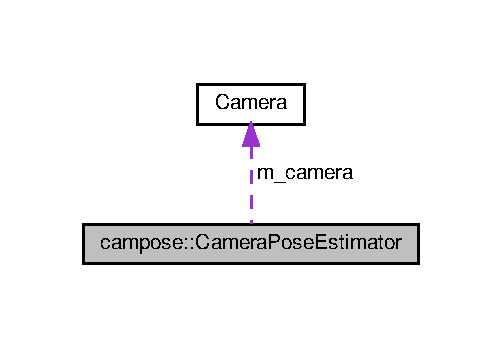
\includegraphics[width=241pt]{classcampose_1_1CameraPoseEstimator__coll__graph}
\end{center}
\end{figure}
\subsection*{Public Member Functions}
\begin{DoxyCompactItemize}
\item 
\hyperlink{classcampose_1_1CameraPoseEstimator_ac2e15d64ea58fbb2fe08b575a599a280}{Camera\+Pose\+Estimator} (const \hyperlink{classCamera}{Camera} \&camera, boost\+::circular\+\_\+buffer$<$ \hyperlink{classFrame}{Frame} $>$ \&frame\+Buffer)
\item 
bool \hyperlink{classcampose_1_1CameraPoseEstimator_a975c193e745e9150f0726e188a2daa1e}{calc\+Camera\+Pose} (const std\+::vector$<$ cv\+::\+Point2f $>$ \&refined\+Points\+Prev, const std\+::vector$<$ cv\+::\+Point2f $>$ \&refined\+Points\+Curr, cv\+::\+Mat \&rotation\+Matrix, cv\+::\+Mat \&translation\+Vector)
\item 
void \hyperlink{classcampose_1_1CameraPoseEstimator_ac1b95d78d7d3f4c8032d8e494034420c}{visualize} ()
\end{DoxyCompactItemize}
\subsection*{Static Public Attributes}
\begin{DoxyCompactItemize}
\item 
static const unsigned int \hyperlink{classcampose_1_1CameraPoseEstimator_ab9495b3f0c0be7276c853bfb97a40f3e}{M\+I\+N\+\_\+\+P\+O\+S\+E\+\_\+\+P\+O\+I\+N\+T\+S\+\_\+\+N\+BR} = 8
\end{DoxyCompactItemize}
\subsection*{Private Attributes}
\begin{DoxyCompactItemize}
\item 
boost\+::circular\+\_\+buffer$<$ \hyperlink{classFrame}{Frame} $>$ \& \hyperlink{classcampose_1_1CameraPoseEstimator_a0e0b0b1b2c9f2c4bbfbc7260021ae723}{m\+\_\+frame\+Buffer}
\item 
\hyperlink{classCamera}{Camera} \hyperlink{classcampose_1_1CameraPoseEstimator_a57173dd1d143e7ac26a039c078204bef}{m\+\_\+camera}
\item 
cv\+::\+Affine3d \hyperlink{classcampose_1_1CameraPoseEstimator_a6afdbcffb70bbe52d945045e1c85fc7d}{m\+\_\+last\+Know\+Pose}
\item 
cv\+::viz\+::\+Viz3d \hyperlink{classcampose_1_1CameraPoseEstimator_a36fa39fcb86bb8758846d1dd0aaa14e9}{m\+\_\+visualizer}
\end{DoxyCompactItemize}


\subsection{Constructor \& Destructor Documentation}
\mbox{\Hypertarget{classcampose_1_1CameraPoseEstimator_ac2e15d64ea58fbb2fe08b575a599a280}\label{classcampose_1_1CameraPoseEstimator_ac2e15d64ea58fbb2fe08b575a599a280}} 
\index{campose\+::\+Camera\+Pose\+Estimator@{campose\+::\+Camera\+Pose\+Estimator}!Camera\+Pose\+Estimator@{Camera\+Pose\+Estimator}}
\index{Camera\+Pose\+Estimator@{Camera\+Pose\+Estimator}!campose\+::\+Camera\+Pose\+Estimator@{campose\+::\+Camera\+Pose\+Estimator}}
\subsubsection{\texorpdfstring{Camera\+Pose\+Estimator()}{CameraPoseEstimator()}}
{\footnotesize\ttfamily campose\+::\+Camera\+Pose\+Estimator\+::\+Camera\+Pose\+Estimator (\begin{DoxyParamCaption}\item[{const \hyperlink{classCamera}{Camera} \&}]{camera,  }\item[{boost\+::circular\+\_\+buffer$<$ \hyperlink{classFrame}{Frame} $>$ \&}]{frame\+Buffer }\end{DoxyParamCaption})\hspace{0.3cm}{\ttfamily [inline]}}

Here is the call graph for this function\+:\nopagebreak
\begin{figure}[H]
\begin{center}
\leavevmode
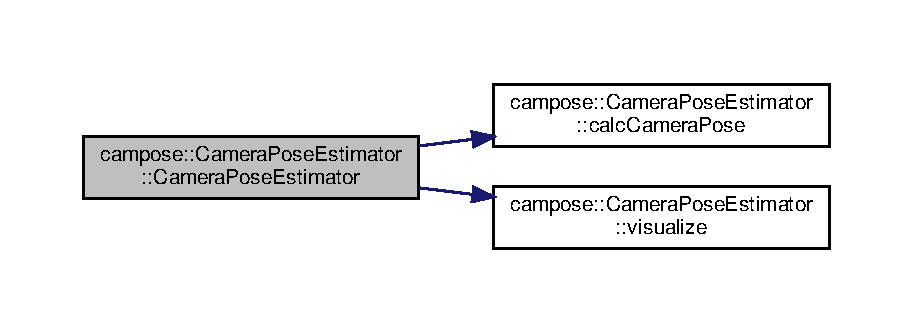
\includegraphics[width=350pt]{classcampose_1_1CameraPoseEstimator_ac2e15d64ea58fbb2fe08b575a599a280_cgraph}
\end{center}
\end{figure}


\subsection{Member Function Documentation}
\mbox{\Hypertarget{classcampose_1_1CameraPoseEstimator_a975c193e745e9150f0726e188a2daa1e}\label{classcampose_1_1CameraPoseEstimator_a975c193e745e9150f0726e188a2daa1e}} 
\index{campose\+::\+Camera\+Pose\+Estimator@{campose\+::\+Camera\+Pose\+Estimator}!calc\+Camera\+Pose@{calc\+Camera\+Pose}}
\index{calc\+Camera\+Pose@{calc\+Camera\+Pose}!campose\+::\+Camera\+Pose\+Estimator@{campose\+::\+Camera\+Pose\+Estimator}}
\subsubsection{\texorpdfstring{calc\+Camera\+Pose()}{calcCameraPose()}}
{\footnotesize\ttfamily bool campose\+::\+Camera\+Pose\+Estimator\+::calc\+Camera\+Pose (\begin{DoxyParamCaption}\item[{const std\+::vector$<$ cv\+::\+Point2f $>$ \&}]{refined\+Points\+Prev,  }\item[{const std\+::vector$<$ cv\+::\+Point2f $>$ \&}]{refined\+Points\+Curr,  }\item[{cv\+::\+Mat \&}]{rotation\+Matrix,  }\item[{cv\+::\+Mat \&}]{translation\+Vector }\end{DoxyParamCaption})}

Here is the caller graph for this function\+:\nopagebreak
\begin{figure}[H]
\begin{center}
\leavevmode
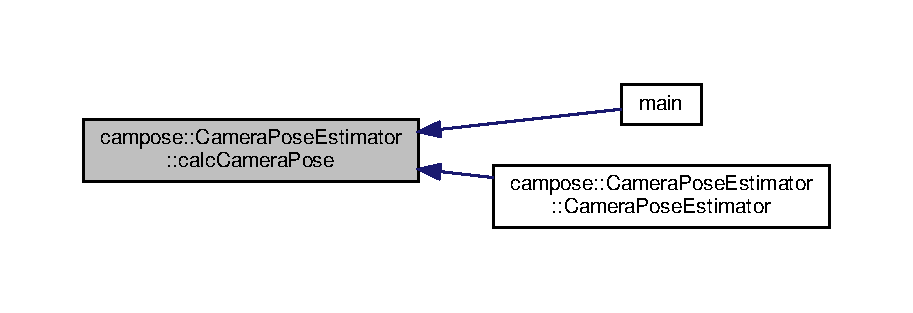
\includegraphics[width=350pt]{classcampose_1_1CameraPoseEstimator_a975c193e745e9150f0726e188a2daa1e_icgraph}
\end{center}
\end{figure}
\mbox{\Hypertarget{classcampose_1_1CameraPoseEstimator_ac1b95d78d7d3f4c8032d8e494034420c}\label{classcampose_1_1CameraPoseEstimator_ac1b95d78d7d3f4c8032d8e494034420c}} 
\index{campose\+::\+Camera\+Pose\+Estimator@{campose\+::\+Camera\+Pose\+Estimator}!visualize@{visualize}}
\index{visualize@{visualize}!campose\+::\+Camera\+Pose\+Estimator@{campose\+::\+Camera\+Pose\+Estimator}}
\subsubsection{\texorpdfstring{visualize()}{visualize()}}
{\footnotesize\ttfamily void Camera\+Pose\+Estimator\+::visualize (\begin{DoxyParamCaption}{ }\end{DoxyParamCaption})}

Here is the caller graph for this function\+:\nopagebreak
\begin{figure}[H]
\begin{center}
\leavevmode
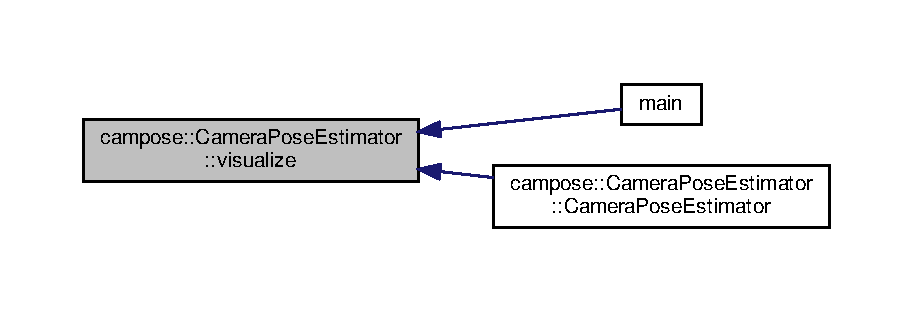
\includegraphics[width=350pt]{classcampose_1_1CameraPoseEstimator_ac1b95d78d7d3f4c8032d8e494034420c_icgraph}
\end{center}
\end{figure}


\subsection{Member Data Documentation}
\mbox{\Hypertarget{classcampose_1_1CameraPoseEstimator_a57173dd1d143e7ac26a039c078204bef}\label{classcampose_1_1CameraPoseEstimator_a57173dd1d143e7ac26a039c078204bef}} 
\index{campose\+::\+Camera\+Pose\+Estimator@{campose\+::\+Camera\+Pose\+Estimator}!m\+\_\+camera@{m\+\_\+camera}}
\index{m\+\_\+camera@{m\+\_\+camera}!campose\+::\+Camera\+Pose\+Estimator@{campose\+::\+Camera\+Pose\+Estimator}}
\subsubsection{\texorpdfstring{m\+\_\+camera}{m\_camera}}
{\footnotesize\ttfamily \hyperlink{classCamera}{Camera} campose\+::\+Camera\+Pose\+Estimator\+::m\+\_\+camera\hspace{0.3cm}{\ttfamily [private]}}

\mbox{\Hypertarget{classcampose_1_1CameraPoseEstimator_a0e0b0b1b2c9f2c4bbfbc7260021ae723}\label{classcampose_1_1CameraPoseEstimator_a0e0b0b1b2c9f2c4bbfbc7260021ae723}} 
\index{campose\+::\+Camera\+Pose\+Estimator@{campose\+::\+Camera\+Pose\+Estimator}!m\+\_\+frame\+Buffer@{m\+\_\+frame\+Buffer}}
\index{m\+\_\+frame\+Buffer@{m\+\_\+frame\+Buffer}!campose\+::\+Camera\+Pose\+Estimator@{campose\+::\+Camera\+Pose\+Estimator}}
\subsubsection{\texorpdfstring{m\+\_\+frame\+Buffer}{m\_frameBuffer}}
{\footnotesize\ttfamily boost\+::circular\+\_\+buffer$<$\hyperlink{classFrame}{Frame}$>$\& campose\+::\+Camera\+Pose\+Estimator\+::m\+\_\+frame\+Buffer\hspace{0.3cm}{\ttfamily [private]}}

\mbox{\Hypertarget{classcampose_1_1CameraPoseEstimator_a6afdbcffb70bbe52d945045e1c85fc7d}\label{classcampose_1_1CameraPoseEstimator_a6afdbcffb70bbe52d945045e1c85fc7d}} 
\index{campose\+::\+Camera\+Pose\+Estimator@{campose\+::\+Camera\+Pose\+Estimator}!m\+\_\+last\+Know\+Pose@{m\+\_\+last\+Know\+Pose}}
\index{m\+\_\+last\+Know\+Pose@{m\+\_\+last\+Know\+Pose}!campose\+::\+Camera\+Pose\+Estimator@{campose\+::\+Camera\+Pose\+Estimator}}
\subsubsection{\texorpdfstring{m\+\_\+last\+Know\+Pose}{m\_lastKnowPose}}
{\footnotesize\ttfamily cv\+::\+Affine3d campose\+::\+Camera\+Pose\+Estimator\+::m\+\_\+last\+Know\+Pose\hspace{0.3cm}{\ttfamily [private]}}

\mbox{\Hypertarget{classcampose_1_1CameraPoseEstimator_a36fa39fcb86bb8758846d1dd0aaa14e9}\label{classcampose_1_1CameraPoseEstimator_a36fa39fcb86bb8758846d1dd0aaa14e9}} 
\index{campose\+::\+Camera\+Pose\+Estimator@{campose\+::\+Camera\+Pose\+Estimator}!m\+\_\+visualizer@{m\+\_\+visualizer}}
\index{m\+\_\+visualizer@{m\+\_\+visualizer}!campose\+::\+Camera\+Pose\+Estimator@{campose\+::\+Camera\+Pose\+Estimator}}
\subsubsection{\texorpdfstring{m\+\_\+visualizer}{m\_visualizer}}
{\footnotesize\ttfamily cv\+::viz\+::\+Viz3d campose\+::\+Camera\+Pose\+Estimator\+::m\+\_\+visualizer\hspace{0.3cm}{\ttfamily [private]}}

\mbox{\Hypertarget{classcampose_1_1CameraPoseEstimator_ab9495b3f0c0be7276c853bfb97a40f3e}\label{classcampose_1_1CameraPoseEstimator_ab9495b3f0c0be7276c853bfb97a40f3e}} 
\index{campose\+::\+Camera\+Pose\+Estimator@{campose\+::\+Camera\+Pose\+Estimator}!M\+I\+N\+\_\+\+P\+O\+S\+E\+\_\+\+P\+O\+I\+N\+T\+S\+\_\+\+N\+BR@{M\+I\+N\+\_\+\+P\+O\+S\+E\+\_\+\+P\+O\+I\+N\+T\+S\+\_\+\+N\+BR}}
\index{M\+I\+N\+\_\+\+P\+O\+S\+E\+\_\+\+P\+O\+I\+N\+T\+S\+\_\+\+N\+BR@{M\+I\+N\+\_\+\+P\+O\+S\+E\+\_\+\+P\+O\+I\+N\+T\+S\+\_\+\+N\+BR}!campose\+::\+Camera\+Pose\+Estimator@{campose\+::\+Camera\+Pose\+Estimator}}
\subsubsection{\texorpdfstring{M\+I\+N\+\_\+\+P\+O\+S\+E\+\_\+\+P\+O\+I\+N\+T\+S\+\_\+\+N\+BR}{MIN\_POSE\_POINTS\_NBR}}
{\footnotesize\ttfamily const unsigned int campose\+::\+Camera\+Pose\+Estimator\+::\+M\+I\+N\+\_\+\+P\+O\+S\+E\+\_\+\+P\+O\+I\+N\+T\+S\+\_\+\+N\+BR = 8\hspace{0.3cm}{\ttfamily [static]}}



The documentation for this class was generated from the following files\+:\begin{DoxyCompactItemize}
\item 
src/pose/\hyperlink{CameraPoseEstimator_8hpp}{Camera\+Pose\+Estimator.\+hpp}\item 
src/pose/\hyperlink{CameraPoseEstimator_8cpp}{Camera\+Pose\+Estimator.\+cpp}\end{DoxyCompactItemize}

\hypertarget{classCameraPoseEstimator}{}\section{Camera\+Pose\+Estimator Class Reference}
\label{classCameraPoseEstimator}\index{Camera\+Pose\+Estimator@{Camera\+Pose\+Estimator}}


{\ttfamily \#include $<$Camera\+Pose\+Estimator2.\+hpp$>$}

\subsection*{Public Member Functions}
\begin{DoxyCompactItemize}
\item 
\hyperlink{classCameraPoseEstimator_a441b62732e43db66f31cb231cd6a0f68}{Camera\+Pose\+Estimator} (boost\+::circular\+\_\+buffer$<$ \hyperlink{structDataFrame}{Data\+Frame} $>$ \&data\+Frame\+Buffer, cv\+::\+Mat camera\+Intri\+Param, cv\+::\+Mat camera\+Distort\+Param, cv\+::viz\+::\+Viz3d \&visualizer)
\item 
void \hyperlink{classCameraPoseEstimator_a2ffa3353dc0ca9913a35c3c018cf19da}{calc\+Camera\+Pose} ()
\item 
void \hyperlink{classCameraPoseEstimator_ac1b95d78d7d3f4c8032d8e494034420c}{visualize} ()
\item 
void \hyperlink{classCameraPoseEstimator_a77d2c2226c4f11ec9e65f3552086abff}{visualize\+Cami} (int i)
\item 
void \hyperlink{classCameraPoseEstimator_af77110f690dea3934f419858cd89fb3b}{visualize\+LastN} (int n)
\item 
void \hyperlink{classCameraPoseEstimator_a8d19513e75924b7e3e56e79a97c534a5}{visualize\+Last\+Frames} ()
\end{DoxyCompactItemize}
\subsection*{Private Attributes}
\begin{DoxyCompactItemize}
\item 
cv\+::\+Mat \hyperlink{classCameraPoseEstimator_a399cc39501f20c5fb80ca5010041ae20}{m\+\_\+\+A\+\_\+calib}
\item 
cv\+::\+Mat \hyperlink{classCameraPoseEstimator_a794f0ecbbbb73d92878c04c757adfe69}{m\+\_\+\+D\+\_\+calib}
\item 
cv\+::\+Matx33f \hyperlink{classCameraPoseEstimator_a8147e1e69f66b58e6d84fa4999045c58}{m\+\_\+\+A\+\_\+calib33f}
\item 
boost\+::circular\+\_\+buffer$<$ \hyperlink{structDataFrame}{Data\+Frame} $>$ \& \hyperlink{classCameraPoseEstimator_aba5c3d97eb6188c08a7b0121c38d1f76}{m\+\_\+data\+Frame\+Buffer}
\item 
cv\+::viz\+::\+Viz3d \hyperlink{classCameraPoseEstimator_ac2465c62e9e4937183fd77e9788d9f8b}{m\+\_\+visualizer}
\item 
bool \hyperlink{classCameraPoseEstimator_a78bb2fadb2826d7ec83d756be0b0fa92}{ena\+\_\+transl\+\_\+factor} =false
\end{DoxyCompactItemize}


\subsection{Constructor \& Destructor Documentation}
\index{Camera\+Pose\+Estimator@{Camera\+Pose\+Estimator}!Camera\+Pose\+Estimator@{Camera\+Pose\+Estimator}}
\index{Camera\+Pose\+Estimator@{Camera\+Pose\+Estimator}!Camera\+Pose\+Estimator@{Camera\+Pose\+Estimator}}
\subsubsection[{\texorpdfstring{Camera\+Pose\+Estimator(boost\+::circular\+\_\+buffer$<$ Data\+Frame $>$ \&data\+Frame\+Buffer, cv\+::\+Mat camera\+Intri\+Param, cv\+::\+Mat camera\+Distort\+Param, cv\+::viz\+::\+Viz3d \&visualizer)}{CameraPoseEstimator(boost::circular_buffer< DataFrame > &dataFrameBuffer, cv::Mat cameraIntriParam, cv::Mat cameraDistortParam, cv::viz::Viz3d &visualizer)}}]{\setlength{\rightskip}{0pt plus 5cm}Camera\+Pose\+Estimator\+::\+Camera\+Pose\+Estimator (
\begin{DoxyParamCaption}
\item[{boost\+::circular\+\_\+buffer$<$ {\bf Data\+Frame} $>$ \&}]{data\+Frame\+Buffer, }
\item[{cv\+::\+Mat}]{camera\+Intri\+Param, }
\item[{cv\+::\+Mat}]{camera\+Distort\+Param, }
\item[{cv\+::viz\+::\+Viz3d \&}]{visualizer}
\end{DoxyParamCaption}
)\hspace{0.3cm}{\ttfamily [inline]}}\hypertarget{classCameraPoseEstimator_a441b62732e43db66f31cb231cd6a0f68}{}\label{classCameraPoseEstimator_a441b62732e43db66f31cb231cd6a0f68}


Here is the call graph for this function\+:\nopagebreak
\begin{figure}[H]
\begin{center}
\leavevmode
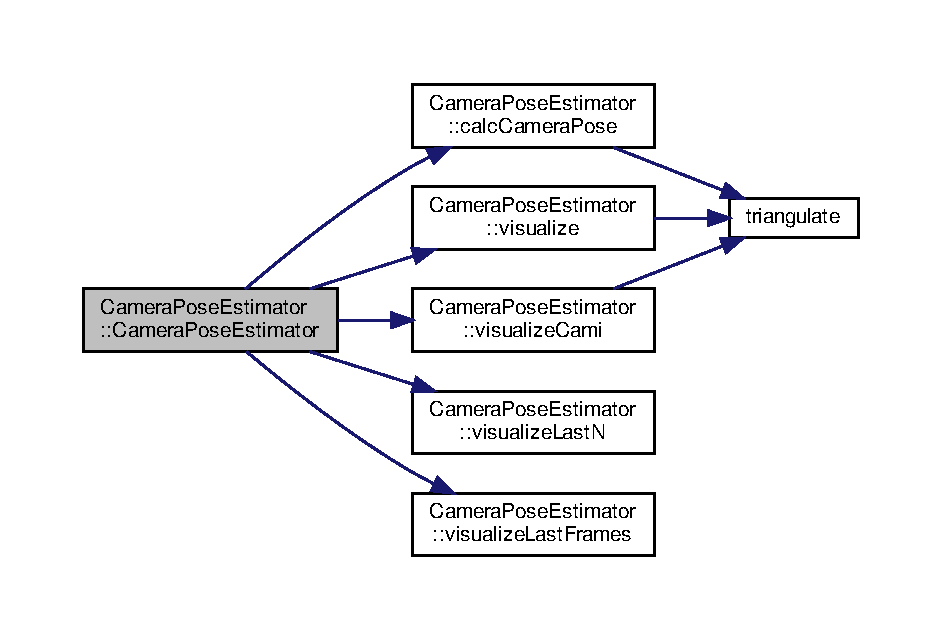
\includegraphics[width=350pt]{classCameraPoseEstimator_a441b62732e43db66f31cb231cd6a0f68_cgraph}
\end{center}
\end{figure}




\subsection{Member Function Documentation}
\index{Camera\+Pose\+Estimator@{Camera\+Pose\+Estimator}!calc\+Camera\+Pose@{calc\+Camera\+Pose}}
\index{calc\+Camera\+Pose@{calc\+Camera\+Pose}!Camera\+Pose\+Estimator@{Camera\+Pose\+Estimator}}
\subsubsection[{\texorpdfstring{calc\+Camera\+Pose()}{calcCameraPose()}}]{\setlength{\rightskip}{0pt plus 5cm}void Camera\+Pose\+Estimator\+::calc\+Camera\+Pose (
\begin{DoxyParamCaption}
{}
\end{DoxyParamCaption}
)}\hypertarget{classCameraPoseEstimator_a2ffa3353dc0ca9913a35c3c018cf19da}{}\label{classCameraPoseEstimator_a2ffa3353dc0ca9913a35c3c018cf19da}


Here is the call graph for this function\+:\nopagebreak
\begin{figure}[H]
\begin{center}
\leavevmode
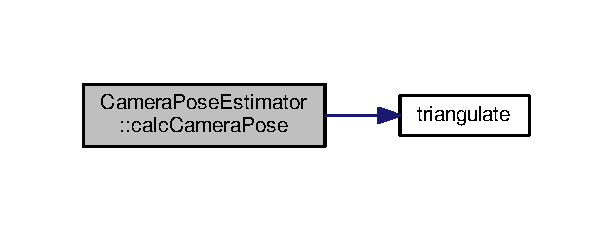
\includegraphics[width=294pt]{classCameraPoseEstimator_a2ffa3353dc0ca9913a35c3c018cf19da_cgraph}
\end{center}
\end{figure}




Here is the caller graph for this function\+:\nopagebreak
\begin{figure}[H]
\begin{center}
\leavevmode
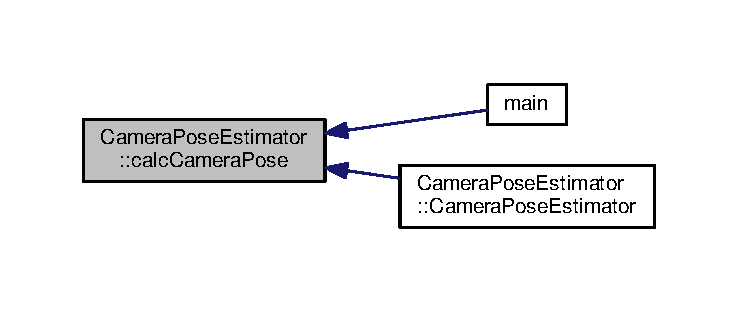
\includegraphics[width=350pt]{classCameraPoseEstimator_a2ffa3353dc0ca9913a35c3c018cf19da_icgraph}
\end{center}
\end{figure}


\index{Camera\+Pose\+Estimator@{Camera\+Pose\+Estimator}!visualize@{visualize}}
\index{visualize@{visualize}!Camera\+Pose\+Estimator@{Camera\+Pose\+Estimator}}
\subsubsection[{\texorpdfstring{visualize()}{visualize()}}]{\setlength{\rightskip}{0pt plus 5cm}void Camera\+Pose\+Estimator\+::visualize (
\begin{DoxyParamCaption}
{}
\end{DoxyParamCaption}
)}\hypertarget{classCameraPoseEstimator_ac1b95d78d7d3f4c8032d8e494034420c}{}\label{classCameraPoseEstimator_ac1b95d78d7d3f4c8032d8e494034420c}
Construct the scene 

Here is the call graph for this function\+:\nopagebreak
\begin{figure}[H]
\begin{center}
\leavevmode
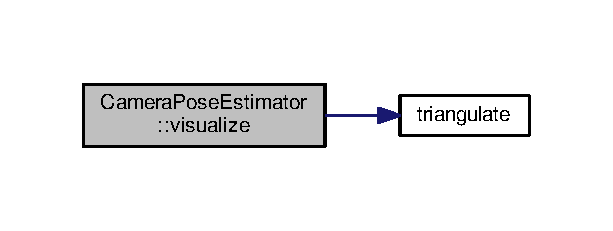
\includegraphics[width=294pt]{classCameraPoseEstimator_ac1b95d78d7d3f4c8032d8e494034420c_cgraph}
\end{center}
\end{figure}




Here is the caller graph for this function\+:\nopagebreak
\begin{figure}[H]
\begin{center}
\leavevmode
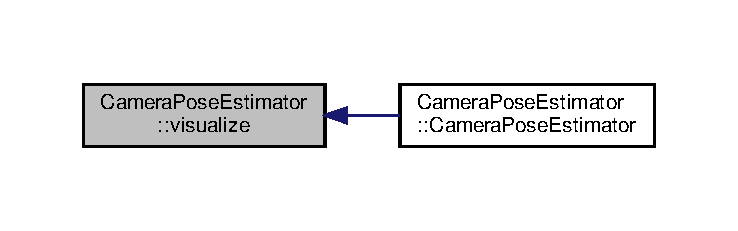
\includegraphics[width=350pt]{classCameraPoseEstimator_ac1b95d78d7d3f4c8032d8e494034420c_icgraph}
\end{center}
\end{figure}


\index{Camera\+Pose\+Estimator@{Camera\+Pose\+Estimator}!visualize\+Cami@{visualize\+Cami}}
\index{visualize\+Cami@{visualize\+Cami}!Camera\+Pose\+Estimator@{Camera\+Pose\+Estimator}}
\subsubsection[{\texorpdfstring{visualize\+Cami(int i)}{visualizeCami(int i)}}]{\setlength{\rightskip}{0pt plus 5cm}void Camera\+Pose\+Estimator\+::visualize\+Cami (
\begin{DoxyParamCaption}
\item[{int}]{i}
\end{DoxyParamCaption}
)}\hypertarget{classCameraPoseEstimator_a77d2c2226c4f11ec9e65f3552086abff}{}\label{classCameraPoseEstimator_a77d2c2226c4f11ec9e65f3552086abff}
Construct the scene 

Here is the call graph for this function\+:\nopagebreak
\begin{figure}[H]
\begin{center}
\leavevmode
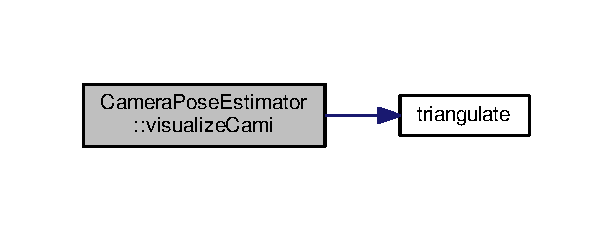
\includegraphics[width=294pt]{classCameraPoseEstimator_a77d2c2226c4f11ec9e65f3552086abff_cgraph}
\end{center}
\end{figure}




Here is the caller graph for this function\+:\nopagebreak
\begin{figure}[H]
\begin{center}
\leavevmode
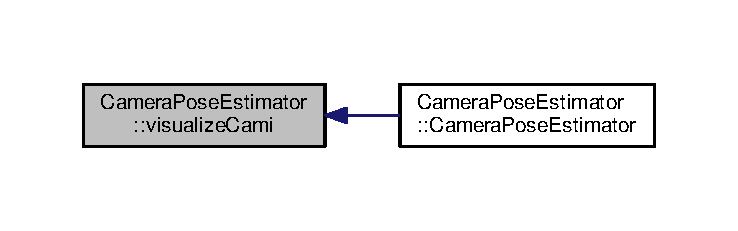
\includegraphics[width=350pt]{classCameraPoseEstimator_a77d2c2226c4f11ec9e65f3552086abff_icgraph}
\end{center}
\end{figure}


\index{Camera\+Pose\+Estimator@{Camera\+Pose\+Estimator}!visualize\+Last\+Frames@{visualize\+Last\+Frames}}
\index{visualize\+Last\+Frames@{visualize\+Last\+Frames}!Camera\+Pose\+Estimator@{Camera\+Pose\+Estimator}}
\subsubsection[{\texorpdfstring{visualize\+Last\+Frames()}{visualizeLastFrames()}}]{\setlength{\rightskip}{0pt plus 5cm}void Camera\+Pose\+Estimator\+::visualize\+Last\+Frames (
\begin{DoxyParamCaption}
{}
\end{DoxyParamCaption}
)}\hypertarget{classCameraPoseEstimator_a8d19513e75924b7e3e56e79a97c534a5}{}\label{classCameraPoseEstimator_a8d19513e75924b7e3e56e79a97c534a5}


Here is the caller graph for this function\+:\nopagebreak
\begin{figure}[H]
\begin{center}
\leavevmode
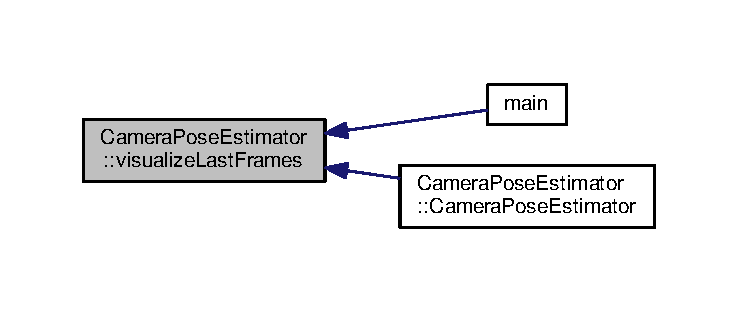
\includegraphics[width=350pt]{classCameraPoseEstimator_a8d19513e75924b7e3e56e79a97c534a5_icgraph}
\end{center}
\end{figure}


\index{Camera\+Pose\+Estimator@{Camera\+Pose\+Estimator}!visualize\+LastN@{visualize\+LastN}}
\index{visualize\+LastN@{visualize\+LastN}!Camera\+Pose\+Estimator@{Camera\+Pose\+Estimator}}
\subsubsection[{\texorpdfstring{visualize\+Last\+N(int n)}{visualizeLastN(int n)}}]{\setlength{\rightskip}{0pt plus 5cm}void Camera\+Pose\+Estimator\+::visualize\+LastN (
\begin{DoxyParamCaption}
\item[{int}]{n}
\end{DoxyParamCaption}
)}\hypertarget{classCameraPoseEstimator_af77110f690dea3934f419858cd89fb3b}{}\label{classCameraPoseEstimator_af77110f690dea3934f419858cd89fb3b}


Here is the caller graph for this function\+:\nopagebreak
\begin{figure}[H]
\begin{center}
\leavevmode
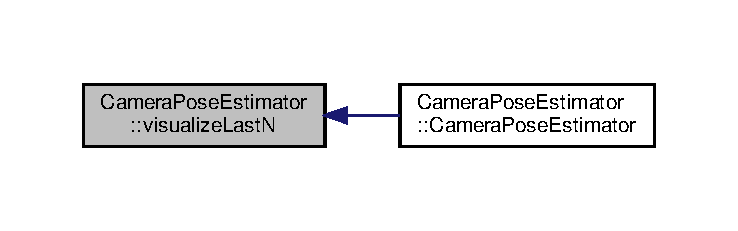
\includegraphics[width=350pt]{classCameraPoseEstimator_af77110f690dea3934f419858cd89fb3b_icgraph}
\end{center}
\end{figure}




\subsection{Member Data Documentation}
\index{Camera\+Pose\+Estimator@{Camera\+Pose\+Estimator}!ena\+\_\+transl\+\_\+factor@{ena\+\_\+transl\+\_\+factor}}
\index{ena\+\_\+transl\+\_\+factor@{ena\+\_\+transl\+\_\+factor}!Camera\+Pose\+Estimator@{Camera\+Pose\+Estimator}}
\subsubsection[{\texorpdfstring{ena\+\_\+transl\+\_\+factor}{ena_transl_factor}}]{\setlength{\rightskip}{0pt plus 5cm}bool Camera\+Pose\+Estimator\+::ena\+\_\+transl\+\_\+factor =false\hspace{0.3cm}{\ttfamily [private]}}\hypertarget{classCameraPoseEstimator_a78bb2fadb2826d7ec83d756be0b0fa92}{}\label{classCameraPoseEstimator_a78bb2fadb2826d7ec83d756be0b0fa92}
\index{Camera\+Pose\+Estimator@{Camera\+Pose\+Estimator}!m\+\_\+\+A\+\_\+calib@{m\+\_\+\+A\+\_\+calib}}
\index{m\+\_\+\+A\+\_\+calib@{m\+\_\+\+A\+\_\+calib}!Camera\+Pose\+Estimator@{Camera\+Pose\+Estimator}}
\subsubsection[{\texorpdfstring{m\+\_\+\+A\+\_\+calib}{m_A_calib}}]{\setlength{\rightskip}{0pt plus 5cm}cv\+::\+Mat Camera\+Pose\+Estimator\+::m\+\_\+\+A\+\_\+calib\hspace{0.3cm}{\ttfamily [private]}}\hypertarget{classCameraPoseEstimator_a399cc39501f20c5fb80ca5010041ae20}{}\label{classCameraPoseEstimator_a399cc39501f20c5fb80ca5010041ae20}
\index{Camera\+Pose\+Estimator@{Camera\+Pose\+Estimator}!m\+\_\+\+A\+\_\+calib33f@{m\+\_\+\+A\+\_\+calib33f}}
\index{m\+\_\+\+A\+\_\+calib33f@{m\+\_\+\+A\+\_\+calib33f}!Camera\+Pose\+Estimator@{Camera\+Pose\+Estimator}}
\subsubsection[{\texorpdfstring{m\+\_\+\+A\+\_\+calib33f}{m_A_calib33f}}]{\setlength{\rightskip}{0pt plus 5cm}cv\+::\+Matx33f Camera\+Pose\+Estimator\+::m\+\_\+\+A\+\_\+calib33f\hspace{0.3cm}{\ttfamily [private]}}\hypertarget{classCameraPoseEstimator_a8147e1e69f66b58e6d84fa4999045c58}{}\label{classCameraPoseEstimator_a8147e1e69f66b58e6d84fa4999045c58}
\index{Camera\+Pose\+Estimator@{Camera\+Pose\+Estimator}!m\+\_\+\+D\+\_\+calib@{m\+\_\+\+D\+\_\+calib}}
\index{m\+\_\+\+D\+\_\+calib@{m\+\_\+\+D\+\_\+calib}!Camera\+Pose\+Estimator@{Camera\+Pose\+Estimator}}
\subsubsection[{\texorpdfstring{m\+\_\+\+D\+\_\+calib}{m_D_calib}}]{\setlength{\rightskip}{0pt plus 5cm}cv\+::\+Mat Camera\+Pose\+Estimator\+::m\+\_\+\+D\+\_\+calib\hspace{0.3cm}{\ttfamily [private]}}\hypertarget{classCameraPoseEstimator_a794f0ecbbbb73d92878c04c757adfe69}{}\label{classCameraPoseEstimator_a794f0ecbbbb73d92878c04c757adfe69}
\index{Camera\+Pose\+Estimator@{Camera\+Pose\+Estimator}!m\+\_\+data\+Frame\+Buffer@{m\+\_\+data\+Frame\+Buffer}}
\index{m\+\_\+data\+Frame\+Buffer@{m\+\_\+data\+Frame\+Buffer}!Camera\+Pose\+Estimator@{Camera\+Pose\+Estimator}}
\subsubsection[{\texorpdfstring{m\+\_\+data\+Frame\+Buffer}{m_dataFrameBuffer}}]{\setlength{\rightskip}{0pt plus 5cm}boost\+::circular\+\_\+buffer$<${\bf Data\+Frame}$>$\& Camera\+Pose\+Estimator\+::m\+\_\+data\+Frame\+Buffer\hspace{0.3cm}{\ttfamily [private]}}\hypertarget{classCameraPoseEstimator_aba5c3d97eb6188c08a7b0121c38d1f76}{}\label{classCameraPoseEstimator_aba5c3d97eb6188c08a7b0121c38d1f76}
\index{Camera\+Pose\+Estimator@{Camera\+Pose\+Estimator}!m\+\_\+visualizer@{m\+\_\+visualizer}}
\index{m\+\_\+visualizer@{m\+\_\+visualizer}!Camera\+Pose\+Estimator@{Camera\+Pose\+Estimator}}
\subsubsection[{\texorpdfstring{m\+\_\+visualizer}{m_visualizer}}]{\setlength{\rightskip}{0pt plus 5cm}cv\+::viz\+::\+Viz3d Camera\+Pose\+Estimator\+::m\+\_\+visualizer\hspace{0.3cm}{\ttfamily [private]}}\hypertarget{classCameraPoseEstimator_ac2465c62e9e4937183fd77e9788d9f8b}{}\label{classCameraPoseEstimator_ac2465c62e9e4937183fd77e9788d9f8b}


The documentation for this class was generated from the following files\+:\begin{DoxyCompactItemize}
\item 
src/pose/\hyperlink{CameraPoseEstimator2_8hpp}{Camera\+Pose\+Estimator2.\+hpp}\item 
src/pose/\hyperlink{CameraPoseEstimator2_8cpp}{Camera\+Pose\+Estimator2.\+cpp}\end{DoxyCompactItemize}

\hypertarget{structDataFrame}{}\section{Data\+Frame Struct Reference}
\label{structDataFrame}\index{Data\+Frame@{Data\+Frame}}


{\ttfamily \#include $<$data\+Structures.\+h$>$}

\subsection*{Public Member Functions}
\begin{DoxyCompactItemize}
\item 
\hyperlink{structDataFrame_a69a9dc47b7506b8062fd34aedacbf579}{Data\+Frame} ()
\end{DoxyCompactItemize}
\subsection*{Public Attributes}
\begin{DoxyCompactItemize}
\item 
cv\+::\+Mat \hyperlink{structDataFrame_ae3261fcdeb3b39c1a4b09bb0c8ce552e}{camera\+Img}
\item 
cv\+::cuda\+::\+Gpu\+Mat \hyperlink{structDataFrame_aca2cdb1fd8ac19b72f29b98157bedf8a}{gpu\+\_\+camera\+Img}
\item 
std\+::vector$<$ cv\+::\+Key\+Point $>$ \hyperlink{structDataFrame_a88fb91bb47cdddd284f2587517856592}{keypoints}
\item 
std\+::vector$<$ cv\+::\+Point2f $>$ \hyperlink{structDataFrame_a2377e8ea584d7e9c1b8207a376cb3ef9}{refined\+Points\+Curr}
\item 
std\+::vector$<$ cv\+::\+Point2f $>$ \hyperlink{structDataFrame_a6dca2985cb4577dc2c672ca027529742}{refined\+Points\+Prev}
\item 
std\+::vector$<$ cv\+::\+Vec2d $>$ \hyperlink{structDataFrame_a47ffc5d8bf594c79163db6c764dc0705}{undistorted\+Points\+Curr}
\item 
std\+::vector$<$ cv\+::\+Vec2d $>$ \hyperlink{structDataFrame_a3725f099035634c1ece2fbdb4dd97256}{undistorted\+Points\+Prev}
\item 
std\+::vector$<$ cv\+::\+Vec3d $>$ \hyperlink{structDataFrame_a1f7311869470a28ac444a9a502b8e5bf}{points3D}
\item 
cv\+::cuda\+::\+Gpu\+Mat \hyperlink{structDataFrame_a2aad6b25c4eec875828841836d69de42}{gpu\+\_\+keypoints}
\item 
cv\+::\+Mat \hyperlink{structDataFrame_aac052b3b741459a8ef04bd768e5e27fa}{descriptors}
\item 
cv\+::cuda\+::\+Gpu\+Mat \hyperlink{structDataFrame_ad2f1e5de380262c6699ef3d674e60005}{gpu\+\_\+descriptors}
\item 
std\+::vector$<$ cv\+::\+D\+Match $>$ \hyperlink{structDataFrame_af551ce74f7dbaa40295c6903c7732dcb}{kpt\+Matches}
\item 
cv\+::cuda\+::\+Gpu\+Mat \hyperlink{structDataFrame_a1b1ff5cf6666f4492af7f4c050a7784e}{gpu\+\_\+kpt\+Matches}
\item 
cv\+::\+Mat \hyperlink{structDataFrame_a04ff1b0f75d65e07490ed8dc24e7e664}{essential\+Matrix}
\item 
cv\+::\+Mat \hyperlink{structDataFrame_afefff04de405c6db0ebc4ed8650b7dfc}{rotation\+Matrix}
\item 
cv\+::\+Mat \hyperlink{structDataFrame_aeda6ec8df72a8df16e984f232b5a27cd}{translation\+Vector}
\item 
cv\+::\+Mat \hyperlink{structDataFrame_a233802c3a35ca0fbee513fab39ee7104}{projection\+Matrix}
\item 
double \hyperlink{structDataFrame_a25ec037466975cee2072b0922effc7f8}{ms\+Timestamp}
\item 
cv\+::\+Affine3d \hyperlink{structDataFrame_a6928232a02166e60d50ef4d551b57d01}{pose}
\item 
int \hyperlink{structDataFrame_a4ca6fd1603f296d7a050f8d47d4ff7a5}{graph\+Prev\+Node}
\end{DoxyCompactItemize}


\subsection{Constructor \& Destructor Documentation}
\index{Data\+Frame@{Data\+Frame}!Data\+Frame@{Data\+Frame}}
\index{Data\+Frame@{Data\+Frame}!Data\+Frame@{Data\+Frame}}
\subsubsection[{\texorpdfstring{Data\+Frame()}{DataFrame()}}]{\setlength{\rightskip}{0pt plus 5cm}Data\+Frame\+::\+Data\+Frame (
\begin{DoxyParamCaption}
{}
\end{DoxyParamCaption}
)\hspace{0.3cm}{\ttfamily [inline]}}\hypertarget{structDataFrame_a69a9dc47b7506b8062fd34aedacbf579}{}\label{structDataFrame_a69a9dc47b7506b8062fd34aedacbf579}


\subsection{Member Data Documentation}
\index{Data\+Frame@{Data\+Frame}!camera\+Img@{camera\+Img}}
\index{camera\+Img@{camera\+Img}!Data\+Frame@{Data\+Frame}}
\subsubsection[{\texorpdfstring{camera\+Img}{cameraImg}}]{\setlength{\rightskip}{0pt plus 5cm}cv\+::\+Mat Data\+Frame\+::camera\+Img}\hypertarget{structDataFrame_ae3261fcdeb3b39c1a4b09bb0c8ce552e}{}\label{structDataFrame_ae3261fcdeb3b39c1a4b09bb0c8ce552e}
\index{Data\+Frame@{Data\+Frame}!descriptors@{descriptors}}
\index{descriptors@{descriptors}!Data\+Frame@{Data\+Frame}}
\subsubsection[{\texorpdfstring{descriptors}{descriptors}}]{\setlength{\rightskip}{0pt plus 5cm}cv\+::\+Mat Data\+Frame\+::descriptors}\hypertarget{structDataFrame_aac052b3b741459a8ef04bd768e5e27fa}{}\label{structDataFrame_aac052b3b741459a8ef04bd768e5e27fa}
\index{Data\+Frame@{Data\+Frame}!essential\+Matrix@{essential\+Matrix}}
\index{essential\+Matrix@{essential\+Matrix}!Data\+Frame@{Data\+Frame}}
\subsubsection[{\texorpdfstring{essential\+Matrix}{essentialMatrix}}]{\setlength{\rightskip}{0pt plus 5cm}cv\+::\+Mat Data\+Frame\+::essential\+Matrix}\hypertarget{structDataFrame_a04ff1b0f75d65e07490ed8dc24e7e664}{}\label{structDataFrame_a04ff1b0f75d65e07490ed8dc24e7e664}
\index{Data\+Frame@{Data\+Frame}!gpu\+\_\+camera\+Img@{gpu\+\_\+camera\+Img}}
\index{gpu\+\_\+camera\+Img@{gpu\+\_\+camera\+Img}!Data\+Frame@{Data\+Frame}}
\subsubsection[{\texorpdfstring{gpu\+\_\+camera\+Img}{gpu_cameraImg}}]{\setlength{\rightskip}{0pt plus 5cm}cv\+::cuda\+::\+Gpu\+Mat Data\+Frame\+::gpu\+\_\+camera\+Img}\hypertarget{structDataFrame_aca2cdb1fd8ac19b72f29b98157bedf8a}{}\label{structDataFrame_aca2cdb1fd8ac19b72f29b98157bedf8a}
\index{Data\+Frame@{Data\+Frame}!gpu\+\_\+descriptors@{gpu\+\_\+descriptors}}
\index{gpu\+\_\+descriptors@{gpu\+\_\+descriptors}!Data\+Frame@{Data\+Frame}}
\subsubsection[{\texorpdfstring{gpu\+\_\+descriptors}{gpu_descriptors}}]{\setlength{\rightskip}{0pt plus 5cm}cv\+::cuda\+::\+Gpu\+Mat Data\+Frame\+::gpu\+\_\+descriptors}\hypertarget{structDataFrame_ad2f1e5de380262c6699ef3d674e60005}{}\label{structDataFrame_ad2f1e5de380262c6699ef3d674e60005}
\index{Data\+Frame@{Data\+Frame}!gpu\+\_\+keypoints@{gpu\+\_\+keypoints}}
\index{gpu\+\_\+keypoints@{gpu\+\_\+keypoints}!Data\+Frame@{Data\+Frame}}
\subsubsection[{\texorpdfstring{gpu\+\_\+keypoints}{gpu_keypoints}}]{\setlength{\rightskip}{0pt plus 5cm}cv\+::cuda\+::\+Gpu\+Mat Data\+Frame\+::gpu\+\_\+keypoints}\hypertarget{structDataFrame_a2aad6b25c4eec875828841836d69de42}{}\label{structDataFrame_a2aad6b25c4eec875828841836d69de42}
\index{Data\+Frame@{Data\+Frame}!gpu\+\_\+kpt\+Matches@{gpu\+\_\+kpt\+Matches}}
\index{gpu\+\_\+kpt\+Matches@{gpu\+\_\+kpt\+Matches}!Data\+Frame@{Data\+Frame}}
\subsubsection[{\texorpdfstring{gpu\+\_\+kpt\+Matches}{gpu_kptMatches}}]{\setlength{\rightskip}{0pt plus 5cm}cv\+::cuda\+::\+Gpu\+Mat Data\+Frame\+::gpu\+\_\+kpt\+Matches}\hypertarget{structDataFrame_a1b1ff5cf6666f4492af7f4c050a7784e}{}\label{structDataFrame_a1b1ff5cf6666f4492af7f4c050a7784e}
\index{Data\+Frame@{Data\+Frame}!graph\+Prev\+Node@{graph\+Prev\+Node}}
\index{graph\+Prev\+Node@{graph\+Prev\+Node}!Data\+Frame@{Data\+Frame}}
\subsubsection[{\texorpdfstring{graph\+Prev\+Node}{graphPrevNode}}]{\setlength{\rightskip}{0pt plus 5cm}int Data\+Frame\+::graph\+Prev\+Node}\hypertarget{structDataFrame_a4ca6fd1603f296d7a050f8d47d4ff7a5}{}\label{structDataFrame_a4ca6fd1603f296d7a050f8d47d4ff7a5}
\index{Data\+Frame@{Data\+Frame}!keypoints@{keypoints}}
\index{keypoints@{keypoints}!Data\+Frame@{Data\+Frame}}
\subsubsection[{\texorpdfstring{keypoints}{keypoints}}]{\setlength{\rightskip}{0pt plus 5cm}std\+::vector$<$cv\+::\+Key\+Point$>$ Data\+Frame\+::keypoints}\hypertarget{structDataFrame_a88fb91bb47cdddd284f2587517856592}{}\label{structDataFrame_a88fb91bb47cdddd284f2587517856592}
\index{Data\+Frame@{Data\+Frame}!kpt\+Matches@{kpt\+Matches}}
\index{kpt\+Matches@{kpt\+Matches}!Data\+Frame@{Data\+Frame}}
\subsubsection[{\texorpdfstring{kpt\+Matches}{kptMatches}}]{\setlength{\rightskip}{0pt plus 5cm}std\+::vector$<$cv\+::\+D\+Match$>$ Data\+Frame\+::kpt\+Matches}\hypertarget{structDataFrame_af551ce74f7dbaa40295c6903c7732dcb}{}\label{structDataFrame_af551ce74f7dbaa40295c6903c7732dcb}
\index{Data\+Frame@{Data\+Frame}!ms\+Timestamp@{ms\+Timestamp}}
\index{ms\+Timestamp@{ms\+Timestamp}!Data\+Frame@{Data\+Frame}}
\subsubsection[{\texorpdfstring{ms\+Timestamp}{msTimestamp}}]{\setlength{\rightskip}{0pt plus 5cm}double Data\+Frame\+::ms\+Timestamp}\hypertarget{structDataFrame_a25ec037466975cee2072b0922effc7f8}{}\label{structDataFrame_a25ec037466975cee2072b0922effc7f8}
\index{Data\+Frame@{Data\+Frame}!points3D@{points3D}}
\index{points3D@{points3D}!Data\+Frame@{Data\+Frame}}
\subsubsection[{\texorpdfstring{points3D}{points3D}}]{\setlength{\rightskip}{0pt plus 5cm}std\+::vector$<$cv\+::\+Vec3d$>$ Data\+Frame\+::points3D}\hypertarget{structDataFrame_a1f7311869470a28ac444a9a502b8e5bf}{}\label{structDataFrame_a1f7311869470a28ac444a9a502b8e5bf}
\index{Data\+Frame@{Data\+Frame}!pose@{pose}}
\index{pose@{pose}!Data\+Frame@{Data\+Frame}}
\subsubsection[{\texorpdfstring{pose}{pose}}]{\setlength{\rightskip}{0pt plus 5cm}cv\+::\+Affine3d Data\+Frame\+::pose}\hypertarget{structDataFrame_a6928232a02166e60d50ef4d551b57d01}{}\label{structDataFrame_a6928232a02166e60d50ef4d551b57d01}
\index{Data\+Frame@{Data\+Frame}!projection\+Matrix@{projection\+Matrix}}
\index{projection\+Matrix@{projection\+Matrix}!Data\+Frame@{Data\+Frame}}
\subsubsection[{\texorpdfstring{projection\+Matrix}{projectionMatrix}}]{\setlength{\rightskip}{0pt plus 5cm}cv\+::\+Mat Data\+Frame\+::projection\+Matrix}\hypertarget{structDataFrame_a233802c3a35ca0fbee513fab39ee7104}{}\label{structDataFrame_a233802c3a35ca0fbee513fab39ee7104}
\index{Data\+Frame@{Data\+Frame}!refined\+Points\+Curr@{refined\+Points\+Curr}}
\index{refined\+Points\+Curr@{refined\+Points\+Curr}!Data\+Frame@{Data\+Frame}}
\subsubsection[{\texorpdfstring{refined\+Points\+Curr}{refinedPointsCurr}}]{\setlength{\rightskip}{0pt plus 5cm}std\+::vector$<$cv\+::\+Point2f$>$ Data\+Frame\+::refined\+Points\+Curr}\hypertarget{structDataFrame_a2377e8ea584d7e9c1b8207a376cb3ef9}{}\label{structDataFrame_a2377e8ea584d7e9c1b8207a376cb3ef9}
\index{Data\+Frame@{Data\+Frame}!refined\+Points\+Prev@{refined\+Points\+Prev}}
\index{refined\+Points\+Prev@{refined\+Points\+Prev}!Data\+Frame@{Data\+Frame}}
\subsubsection[{\texorpdfstring{refined\+Points\+Prev}{refinedPointsPrev}}]{\setlength{\rightskip}{0pt plus 5cm}std\+::vector$<$cv\+::\+Point2f$>$ Data\+Frame\+::refined\+Points\+Prev}\hypertarget{structDataFrame_a6dca2985cb4577dc2c672ca027529742}{}\label{structDataFrame_a6dca2985cb4577dc2c672ca027529742}
\index{Data\+Frame@{Data\+Frame}!rotation\+Matrix@{rotation\+Matrix}}
\index{rotation\+Matrix@{rotation\+Matrix}!Data\+Frame@{Data\+Frame}}
\subsubsection[{\texorpdfstring{rotation\+Matrix}{rotationMatrix}}]{\setlength{\rightskip}{0pt plus 5cm}cv\+::\+Mat Data\+Frame\+::rotation\+Matrix}\hypertarget{structDataFrame_afefff04de405c6db0ebc4ed8650b7dfc}{}\label{structDataFrame_afefff04de405c6db0ebc4ed8650b7dfc}
\index{Data\+Frame@{Data\+Frame}!translation\+Vector@{translation\+Vector}}
\index{translation\+Vector@{translation\+Vector}!Data\+Frame@{Data\+Frame}}
\subsubsection[{\texorpdfstring{translation\+Vector}{translationVector}}]{\setlength{\rightskip}{0pt plus 5cm}cv\+::\+Mat Data\+Frame\+::translation\+Vector}\hypertarget{structDataFrame_aeda6ec8df72a8df16e984f232b5a27cd}{}\label{structDataFrame_aeda6ec8df72a8df16e984f232b5a27cd}
\index{Data\+Frame@{Data\+Frame}!undistorted\+Points\+Curr@{undistorted\+Points\+Curr}}
\index{undistorted\+Points\+Curr@{undistorted\+Points\+Curr}!Data\+Frame@{Data\+Frame}}
\subsubsection[{\texorpdfstring{undistorted\+Points\+Curr}{undistortedPointsCurr}}]{\setlength{\rightskip}{0pt plus 5cm}std\+::vector$<$cv\+::\+Vec2d$>$ Data\+Frame\+::undistorted\+Points\+Curr}\hypertarget{structDataFrame_a47ffc5d8bf594c79163db6c764dc0705}{}\label{structDataFrame_a47ffc5d8bf594c79163db6c764dc0705}
\index{Data\+Frame@{Data\+Frame}!undistorted\+Points\+Prev@{undistorted\+Points\+Prev}}
\index{undistorted\+Points\+Prev@{undistorted\+Points\+Prev}!Data\+Frame@{Data\+Frame}}
\subsubsection[{\texorpdfstring{undistorted\+Points\+Prev}{undistortedPointsPrev}}]{\setlength{\rightskip}{0pt plus 5cm}std\+::vector$<$cv\+::\+Vec2d$>$ Data\+Frame\+::undistorted\+Points\+Prev}\hypertarget{structDataFrame_a3725f099035634c1ece2fbdb4dd97256}{}\label{structDataFrame_a3725f099035634c1ece2fbdb4dd97256}


The documentation for this struct was generated from the following file\+:\begin{DoxyCompactItemize}
\item 
src/frame/\hyperlink{dataStructures_8h}{data\+Structures.\+h}\end{DoxyCompactItemize}

\hypertarget{classFrame}{}\section{Frame Class Reference}
\label{classFrame}\index{Frame@{Frame}}


{\ttfamily \#include $<$Frame.\+hpp$>$}

\subsection*{Public Member Functions}
\begin{DoxyCompactItemize}
\item 
\hyperlink{classFrame_af76c0928474fc6132e92511d8ac0791d}{Frame} (cv\+::\+Mat input\+Image)
\item 
{\footnotesize template$<$class Archive $>$ }\\void \hyperlink{classFrame_a2ad8e5090a32bab1894f2dcd84e50512}{serialize} (Archive \&ar, const unsigned int version)
\end{DoxyCompactItemize}
\subsection*{Public Attributes}
\begin{DoxyCompactItemize}
\item 
cv\+::\+Mat \hyperlink{classFrame_af327ba7e56d6e4cd8f2917d36284ca4c}{camera\+Img}
\item 
double \hyperlink{classFrame_a360891231ed2b244f6caf3cfc8c16fb5}{timestamp}
\item 
std\+::vector$<$ cv\+::\+Key\+Point $>$ \hyperlink{classFrame_aec3f6874598eadb1e014709b28e48061}{keypoints}
\item 
std\+::vector$<$ cv\+::\+D\+Match $>$ \hyperlink{classFrame_ac7224127d7700699319bc8a8e84bef23}{matches}
\item 
std\+::vector$<$ cv\+::\+Point2f $>$ \hyperlink{classFrame_aee50f053bed60891e4582e3a478bcc1d}{refined\+Points\+Curr}
\item 
cv\+::\+Mat \hyperlink{classFrame_a358eda120b8420754f30f69007e9fecb}{descriptors}
\item 
std\+::vector$<$ cv\+::\+Point2f $>$ \hyperlink{classFrame_a548f00afc5984a717684cc2916c0bd4c}{refined\+Points\+Prev}
\item 
std\+::vector$<$ cv\+::\+Vec2d $>$ \hyperlink{classFrame_a81aae40549c6b5548cf63d050f7a19e3}{undistorted\+Points\+Curr}
\item 
std\+::vector$<$ cv\+::\+Vec2d $>$ \hyperlink{classFrame_a9efe87123d623bfe06327036ee59e423}{undistorted\+Points\+Prev}
\item 
std\+::vector$<$ cv\+::\+Vec3d $>$ \hyperlink{classFrame_a387c7eff30bc00e6375fd9efa5510d22}{points3D}
\item 
cv\+::\+Mat \hyperlink{classFrame_a07cc311d7b6e3dd5b964a4ea42a003b3}{essential\+Matrix}
\item 
cv\+::\+Mat \hyperlink{classFrame_ae6b2810e1e9d8cc8a5ba7dff9378b019}{rotation\+Matrix}
\item 
cv\+::\+Mat \hyperlink{classFrame_a5635d2b68ffd5456f6e7ad0f54d1ba29}{translation\+Vector}
\item 
cv\+::\+Mat \hyperlink{classFrame_acc5cd57f6b94c159a2f80ff6416dfb25}{projection\+Matrix}
\end{DoxyCompactItemize}
\subsection*{Friends}
\begin{DoxyCompactItemize}
\item 
class \hyperlink{classFrame_ac98d07dd8f7b70e16ccb9a01abf56b9c}{boost\+::serialization\+::access}
\end{DoxyCompactItemize}


\subsection{Constructor \& Destructor Documentation}
\mbox{\Hypertarget{classFrame_af76c0928474fc6132e92511d8ac0791d}\label{classFrame_af76c0928474fc6132e92511d8ac0791d}} 
\index{Frame@{Frame}!Frame@{Frame}}
\index{Frame@{Frame}!Frame@{Frame}}
\subsubsection{\texorpdfstring{Frame()}{Frame()}}
{\footnotesize\ttfamily Frame\+::\+Frame (\begin{DoxyParamCaption}\item[{cv\+::\+Mat}]{input\+Image }\end{DoxyParamCaption})\hspace{0.3cm}{\ttfamily [inline]}}



\subsection{Member Function Documentation}
\mbox{\Hypertarget{classFrame_a2ad8e5090a32bab1894f2dcd84e50512}\label{classFrame_a2ad8e5090a32bab1894f2dcd84e50512}} 
\index{Frame@{Frame}!serialize@{serialize}}
\index{serialize@{serialize}!Frame@{Frame}}
\subsubsection{\texorpdfstring{serialize()}{serialize()}}
{\footnotesize\ttfamily template$<$class Archive $>$ \\
void Frame\+::serialize (\begin{DoxyParamCaption}\item[{Archive \&}]{ar,  }\item[{const unsigned int}]{version }\end{DoxyParamCaption})\hspace{0.3cm}{\ttfamily [inline]}}



\subsection{Friends And Related Function Documentation}
\mbox{\Hypertarget{classFrame_ac98d07dd8f7b70e16ccb9a01abf56b9c}\label{classFrame_ac98d07dd8f7b70e16ccb9a01abf56b9c}} 
\index{Frame@{Frame}!boost\+::serialization\+::access@{boost\+::serialization\+::access}}
\index{boost\+::serialization\+::access@{boost\+::serialization\+::access}!Frame@{Frame}}
\subsubsection{\texorpdfstring{boost\+::serialization\+::access}{boost::serialization::access}}
{\footnotesize\ttfamily friend class boost\+::serialization\+::access\hspace{0.3cm}{\ttfamily [friend]}}



\subsection{Member Data Documentation}
\mbox{\Hypertarget{classFrame_af327ba7e56d6e4cd8f2917d36284ca4c}\label{classFrame_af327ba7e56d6e4cd8f2917d36284ca4c}} 
\index{Frame@{Frame}!camera\+Img@{camera\+Img}}
\index{camera\+Img@{camera\+Img}!Frame@{Frame}}
\subsubsection{\texorpdfstring{camera\+Img}{cameraImg}}
{\footnotesize\ttfamily cv\+::\+Mat Frame\+::camera\+Img}

\mbox{\Hypertarget{classFrame_a358eda120b8420754f30f69007e9fecb}\label{classFrame_a358eda120b8420754f30f69007e9fecb}} 
\index{Frame@{Frame}!descriptors@{descriptors}}
\index{descriptors@{descriptors}!Frame@{Frame}}
\subsubsection{\texorpdfstring{descriptors}{descriptors}}
{\footnotesize\ttfamily cv\+::\+Mat Frame\+::descriptors}

\mbox{\Hypertarget{classFrame_a07cc311d7b6e3dd5b964a4ea42a003b3}\label{classFrame_a07cc311d7b6e3dd5b964a4ea42a003b3}} 
\index{Frame@{Frame}!essential\+Matrix@{essential\+Matrix}}
\index{essential\+Matrix@{essential\+Matrix}!Frame@{Frame}}
\subsubsection{\texorpdfstring{essential\+Matrix}{essentialMatrix}}
{\footnotesize\ttfamily cv\+::\+Mat Frame\+::essential\+Matrix}

\mbox{\Hypertarget{classFrame_aec3f6874598eadb1e014709b28e48061}\label{classFrame_aec3f6874598eadb1e014709b28e48061}} 
\index{Frame@{Frame}!keypoints@{keypoints}}
\index{keypoints@{keypoints}!Frame@{Frame}}
\subsubsection{\texorpdfstring{keypoints}{keypoints}}
{\footnotesize\ttfamily std\+::vector$<$cv\+::\+Key\+Point$>$ Frame\+::keypoints}

\mbox{\Hypertarget{classFrame_ac7224127d7700699319bc8a8e84bef23}\label{classFrame_ac7224127d7700699319bc8a8e84bef23}} 
\index{Frame@{Frame}!matches@{matches}}
\index{matches@{matches}!Frame@{Frame}}
\subsubsection{\texorpdfstring{matches}{matches}}
{\footnotesize\ttfamily std\+::vector$<$ cv\+::\+D\+Match $>$ Frame\+::matches}

\mbox{\Hypertarget{classFrame_a387c7eff30bc00e6375fd9efa5510d22}\label{classFrame_a387c7eff30bc00e6375fd9efa5510d22}} 
\index{Frame@{Frame}!points3D@{points3D}}
\index{points3D@{points3D}!Frame@{Frame}}
\subsubsection{\texorpdfstring{points3D}{points3D}}
{\footnotesize\ttfamily std\+::vector$<$cv\+::\+Vec3d$>$ Frame\+::points3D}

\mbox{\Hypertarget{classFrame_acc5cd57f6b94c159a2f80ff6416dfb25}\label{classFrame_acc5cd57f6b94c159a2f80ff6416dfb25}} 
\index{Frame@{Frame}!projection\+Matrix@{projection\+Matrix}}
\index{projection\+Matrix@{projection\+Matrix}!Frame@{Frame}}
\subsubsection{\texorpdfstring{projection\+Matrix}{projectionMatrix}}
{\footnotesize\ttfamily cv\+::\+Mat Frame\+::projection\+Matrix}

\mbox{\Hypertarget{classFrame_aee50f053bed60891e4582e3a478bcc1d}\label{classFrame_aee50f053bed60891e4582e3a478bcc1d}} 
\index{Frame@{Frame}!refined\+Points\+Curr@{refined\+Points\+Curr}}
\index{refined\+Points\+Curr@{refined\+Points\+Curr}!Frame@{Frame}}
\subsubsection{\texorpdfstring{refined\+Points\+Curr}{refinedPointsCurr}}
{\footnotesize\ttfamily std\+::vector$<$cv\+::\+Point2f$>$ Frame\+::refined\+Points\+Curr}

\mbox{\Hypertarget{classFrame_a548f00afc5984a717684cc2916c0bd4c}\label{classFrame_a548f00afc5984a717684cc2916c0bd4c}} 
\index{Frame@{Frame}!refined\+Points\+Prev@{refined\+Points\+Prev}}
\index{refined\+Points\+Prev@{refined\+Points\+Prev}!Frame@{Frame}}
\subsubsection{\texorpdfstring{refined\+Points\+Prev}{refinedPointsPrev}}
{\footnotesize\ttfamily std\+::vector$<$cv\+::\+Point2f$>$ Frame\+::refined\+Points\+Prev}

\mbox{\Hypertarget{classFrame_ae6b2810e1e9d8cc8a5ba7dff9378b019}\label{classFrame_ae6b2810e1e9d8cc8a5ba7dff9378b019}} 
\index{Frame@{Frame}!rotation\+Matrix@{rotation\+Matrix}}
\index{rotation\+Matrix@{rotation\+Matrix}!Frame@{Frame}}
\subsubsection{\texorpdfstring{rotation\+Matrix}{rotationMatrix}}
{\footnotesize\ttfamily cv\+::\+Mat Frame\+::rotation\+Matrix}

\mbox{\Hypertarget{classFrame_a360891231ed2b244f6caf3cfc8c16fb5}\label{classFrame_a360891231ed2b244f6caf3cfc8c16fb5}} 
\index{Frame@{Frame}!timestamp@{timestamp}}
\index{timestamp@{timestamp}!Frame@{Frame}}
\subsubsection{\texorpdfstring{timestamp}{timestamp}}
{\footnotesize\ttfamily double Frame\+::timestamp}

\mbox{\Hypertarget{classFrame_a5635d2b68ffd5456f6e7ad0f54d1ba29}\label{classFrame_a5635d2b68ffd5456f6e7ad0f54d1ba29}} 
\index{Frame@{Frame}!translation\+Vector@{translation\+Vector}}
\index{translation\+Vector@{translation\+Vector}!Frame@{Frame}}
\subsubsection{\texorpdfstring{translation\+Vector}{translationVector}}
{\footnotesize\ttfamily cv\+::\+Mat Frame\+::translation\+Vector}

\mbox{\Hypertarget{classFrame_a81aae40549c6b5548cf63d050f7a19e3}\label{classFrame_a81aae40549c6b5548cf63d050f7a19e3}} 
\index{Frame@{Frame}!undistorted\+Points\+Curr@{undistorted\+Points\+Curr}}
\index{undistorted\+Points\+Curr@{undistorted\+Points\+Curr}!Frame@{Frame}}
\subsubsection{\texorpdfstring{undistorted\+Points\+Curr}{undistortedPointsCurr}}
{\footnotesize\ttfamily std\+::vector$<$cv\+::\+Vec2d$>$ Frame\+::undistorted\+Points\+Curr}

\mbox{\Hypertarget{classFrame_a9efe87123d623bfe06327036ee59e423}\label{classFrame_a9efe87123d623bfe06327036ee59e423}} 
\index{Frame@{Frame}!undistorted\+Points\+Prev@{undistorted\+Points\+Prev}}
\index{undistorted\+Points\+Prev@{undistorted\+Points\+Prev}!Frame@{Frame}}
\subsubsection{\texorpdfstring{undistorted\+Points\+Prev}{undistortedPointsPrev}}
{\footnotesize\ttfamily std\+::vector$<$cv\+::\+Vec2d$>$ Frame\+::undistorted\+Points\+Prev}



The documentation for this class was generated from the following file\+:\begin{DoxyCompactItemize}
\item 
src/frame/\hyperlink{Frame_8hpp}{Frame.\+hpp}\end{DoxyCompactItemize}

\hypertarget{classFrameProvider}{}\section{Frame\+Provider Class Reference}
\label{classFrameProvider}\index{Frame\+Provider@{Frame\+Provider}}


{\ttfamily \#include $<$Frame\+Provider.\+hpp$>$}

\subsection*{Public Member Functions}
\begin{DoxyCompactItemize}
\item 
\hyperlink{classFrameProvider_a03f142a7ea5878a32fec67f2b85f22fd}{Frame\+Provider} (std\+::mutex \&\hyperlink{campose__images__kitty__main2_8cpp_a29ac681ec3efa9e30e1ab1ab251b47f9}{mtx}, bool \&frame\+Avail, cv\+::\+Mat \&frame)
\item 
void \hyperlink{classFrameProvider_aa8334a484db470ee01b8718ab05ca997}{capture\+Frames\+From\+Folder} (const std\+::string folder\+Path, size\+\_\+t start\+Idx, size\+\_\+t end\+Idx)
\item 
void \hyperlink{classFrameProvider_a15097906b20d2d564b9bfea82c2f956c}{capture\+Frames\+From\+Argus\+Cam} ()
\end{DoxyCompactItemize}
\subsection*{Private Attributes}
\begin{DoxyCompactItemize}
\item 
std\+::thread $\ast$ \hyperlink{classFrameProvider_a08d38afae37b22f5c0117bdc950d83b4}{m\+\_\+capture\+Frame\+Thread}
\item 
std\+::mutex \& \hyperlink{classFrameProvider_a613fbc156614a7936ef4e05d8c9b0219}{m\+\_\+mutex}
\item 
bool \& \hyperlink{classFrameProvider_a46df01a978cd8d56cd4ffafb676d8a44}{m\+\_\+frame\+Available}
\item 
cv\+::\+Mat \& \hyperlink{classFrameProvider_afc074a4806d6406cbb395f98494a2172}{m\+\_\+frame}
\end{DoxyCompactItemize}


\subsection{Constructor \& Destructor Documentation}
\mbox{\Hypertarget{classFrameProvider_a03f142a7ea5878a32fec67f2b85f22fd}\label{classFrameProvider_a03f142a7ea5878a32fec67f2b85f22fd}} 
\index{Frame\+Provider@{Frame\+Provider}!Frame\+Provider@{Frame\+Provider}}
\index{Frame\+Provider@{Frame\+Provider}!Frame\+Provider@{Frame\+Provider}}
\subsubsection{\texorpdfstring{Frame\+Provider()}{FrameProvider()}}
{\footnotesize\ttfamily Frame\+Provider\+::\+Frame\+Provider (\begin{DoxyParamCaption}\item[{std\+::mutex \&}]{mtx,  }\item[{bool \&}]{frame\+Avail,  }\item[{cv\+::\+Mat \&}]{frame }\end{DoxyParamCaption})\hspace{0.3cm}{\ttfamily [inline]}}

Here is the call graph for this function\+:\nopagebreak
\begin{figure}[H]
\begin{center}
\leavevmode
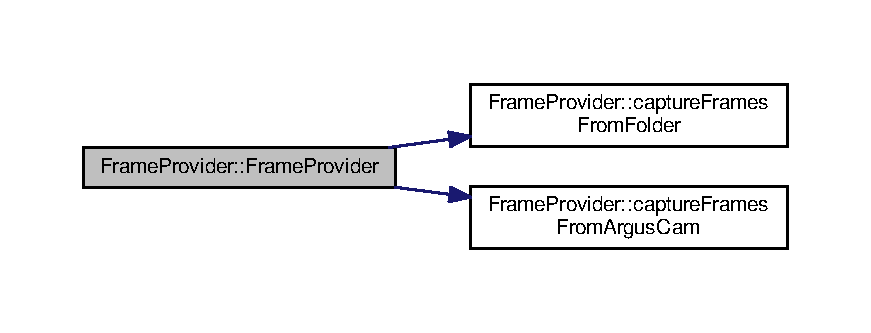
\includegraphics[width=350pt]{classFrameProvider_a03f142a7ea5878a32fec67f2b85f22fd_cgraph}
\end{center}
\end{figure}


\subsection{Member Function Documentation}
\mbox{\Hypertarget{classFrameProvider_a15097906b20d2d564b9bfea82c2f956c}\label{classFrameProvider_a15097906b20d2d564b9bfea82c2f956c}} 
\index{Frame\+Provider@{Frame\+Provider}!capture\+Frames\+From\+Argus\+Cam@{capture\+Frames\+From\+Argus\+Cam}}
\index{capture\+Frames\+From\+Argus\+Cam@{capture\+Frames\+From\+Argus\+Cam}!Frame\+Provider@{Frame\+Provider}}
\subsubsection{\texorpdfstring{capture\+Frames\+From\+Argus\+Cam()}{captureFramesFromArgusCam()}}
{\footnotesize\ttfamily void Frame\+Provider\+::capture\+Frames\+From\+Argus\+Cam (\begin{DoxyParamCaption}{ }\end{DoxyParamCaption})}

Here is the caller graph for this function\+:\nopagebreak
\begin{figure}[H]
\begin{center}
\leavevmode
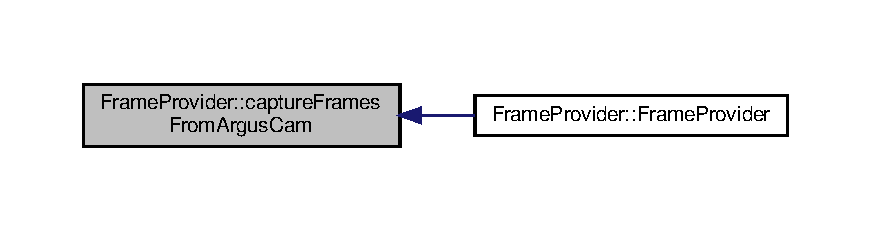
\includegraphics[width=350pt]{classFrameProvider_a15097906b20d2d564b9bfea82c2f956c_icgraph}
\end{center}
\end{figure}
\mbox{\Hypertarget{classFrameProvider_aa8334a484db470ee01b8718ab05ca997}\label{classFrameProvider_aa8334a484db470ee01b8718ab05ca997}} 
\index{Frame\+Provider@{Frame\+Provider}!capture\+Frames\+From\+Folder@{capture\+Frames\+From\+Folder}}
\index{capture\+Frames\+From\+Folder@{capture\+Frames\+From\+Folder}!Frame\+Provider@{Frame\+Provider}}
\subsubsection{\texorpdfstring{capture\+Frames\+From\+Folder()}{captureFramesFromFolder()}}
{\footnotesize\ttfamily void Frame\+Provider\+::capture\+Frames\+From\+Folder (\begin{DoxyParamCaption}\item[{const std\+::string}]{folder\+Path,  }\item[{size\+\_\+t}]{start\+Idx,  }\item[{size\+\_\+t}]{end\+Idx }\end{DoxyParamCaption})}

Here is the caller graph for this function\+:\nopagebreak
\begin{figure}[H]
\begin{center}
\leavevmode
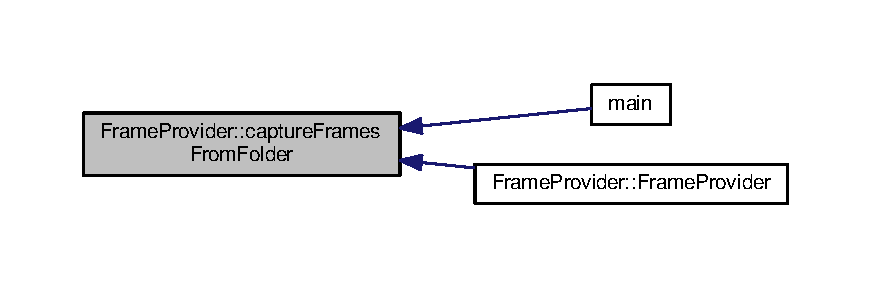
\includegraphics[width=350pt]{classFrameProvider_aa8334a484db470ee01b8718ab05ca997_icgraph}
\end{center}
\end{figure}


\subsection{Member Data Documentation}
\mbox{\Hypertarget{classFrameProvider_a08d38afae37b22f5c0117bdc950d83b4}\label{classFrameProvider_a08d38afae37b22f5c0117bdc950d83b4}} 
\index{Frame\+Provider@{Frame\+Provider}!m\+\_\+capture\+Frame\+Thread@{m\+\_\+capture\+Frame\+Thread}}
\index{m\+\_\+capture\+Frame\+Thread@{m\+\_\+capture\+Frame\+Thread}!Frame\+Provider@{Frame\+Provider}}
\subsubsection{\texorpdfstring{m\+\_\+capture\+Frame\+Thread}{m\_captureFrameThread}}
{\footnotesize\ttfamily std\+::thread$\ast$ Frame\+Provider\+::m\+\_\+capture\+Frame\+Thread\hspace{0.3cm}{\ttfamily [private]}}

\mbox{\Hypertarget{classFrameProvider_afc074a4806d6406cbb395f98494a2172}\label{classFrameProvider_afc074a4806d6406cbb395f98494a2172}} 
\index{Frame\+Provider@{Frame\+Provider}!m\+\_\+frame@{m\+\_\+frame}}
\index{m\+\_\+frame@{m\+\_\+frame}!Frame\+Provider@{Frame\+Provider}}
\subsubsection{\texorpdfstring{m\+\_\+frame}{m\_frame}}
{\footnotesize\ttfamily cv\+::\+Mat\& Frame\+Provider\+::m\+\_\+frame\hspace{0.3cm}{\ttfamily [private]}}

\mbox{\Hypertarget{classFrameProvider_a46df01a978cd8d56cd4ffafb676d8a44}\label{classFrameProvider_a46df01a978cd8d56cd4ffafb676d8a44}} 
\index{Frame\+Provider@{Frame\+Provider}!m\+\_\+frame\+Available@{m\+\_\+frame\+Available}}
\index{m\+\_\+frame\+Available@{m\+\_\+frame\+Available}!Frame\+Provider@{Frame\+Provider}}
\subsubsection{\texorpdfstring{m\+\_\+frame\+Available}{m\_frameAvailable}}
{\footnotesize\ttfamily bool\& Frame\+Provider\+::m\+\_\+frame\+Available\hspace{0.3cm}{\ttfamily [private]}}

\mbox{\Hypertarget{classFrameProvider_a613fbc156614a7936ef4e05d8c9b0219}\label{classFrameProvider_a613fbc156614a7936ef4e05d8c9b0219}} 
\index{Frame\+Provider@{Frame\+Provider}!m\+\_\+mutex@{m\+\_\+mutex}}
\index{m\+\_\+mutex@{m\+\_\+mutex}!Frame\+Provider@{Frame\+Provider}}
\subsubsection{\texorpdfstring{m\+\_\+mutex}{m\_mutex}}
{\footnotesize\ttfamily std\+::mutex\& Frame\+Provider\+::m\+\_\+mutex\hspace{0.3cm}{\ttfamily [private]}}



The documentation for this class was generated from the following files\+:\begin{DoxyCompactItemize}
\item 
src/frame/\hyperlink{FrameProvider_8hpp}{Frame\+Provider.\+hpp}\item 
src/frame/\hyperlink{FrameProvider_8cpp}{Frame\+Provider.\+cpp}\end{DoxyCompactItemize}

\hypertarget{classKeypointProcessorGpu}{}\section{Keypoint\+Processor\+Gpu Class Reference}
\label{classKeypointProcessorGpu}\index{Keypoint\+Processor\+Gpu@{Keypoint\+Processor\+Gpu}}


{\ttfamily \#include $<$Keypoint\+Processor\+Gpu.\+hpp$>$}

\subsection*{Public Member Functions}
\begin{DoxyCompactItemize}
\item 
\hyperlink{classKeypointProcessorGpu_ad08f4085504007fd8a96b4bdd8ee3ecc}{Keypoint\+Processor\+Gpu} (boost\+::circular\+\_\+buffer$<$ \hyperlink{structDataFrame}{Data\+Frame} $>$ \&data\+Frame\+Buffer, std\+::string detector\+Type=\char`\"{}O\+RB\char`\"{}, std\+::string selector\+Type=\char`\"{}S\+E\+L\+\_\+\+K\+NN\char`\"{}, bool use\+G\+P\+Us=false, bool visu\+Enable=false)
\item 
\hyperlink{namespaceExtractReturnCode_a88d3d56de717f250bf48793769dd57ba}{Extract\+Return\+Code\+::\+Extract\+Return\+Code} \hyperlink{classKeypointProcessorGpu_a927a3d8480e8da505524c354e5c02c83}{extract\+Kpoint\+Descriptors} (cv\+::\+Mat \&new\+Image)
\item 
void \hyperlink{classKeypointProcessorGpu_af195f83c19b58a9fedeb50ac3baaa8b3}{match\+Kpoints} (std\+::string mpoint\+Strategy=\char`\"{}F\+U\+ND\char`\"{})
\item 
\hyperlink{namespaceRefineReturnCode_a54e2cd5f4af90ff2df55bf63455d1959}{Refine\+Return\+Code\+::\+Refine\+Return\+Code} \hyperlink{classKeypointProcessorGpu_abdbb860bb800e122dee4c76fcf596fc5}{refine\+Matches} (const std\+::vector$<$ cv\+::\+D\+Match $>$ \&matches, std\+::vector$<$ cv\+::\+Key\+Point $>$ \&keypoints1, std\+::vector$<$ cv\+::\+Key\+Point $>$ \&keypoints2, std\+::vector$<$ cv\+::\+D\+Match $>$ \&out\+Matches, std\+::string match\+Refine\+Strategy)
\item 
void \hyperlink{classKeypointProcessorGpu_a192bc98425b2bc0bea56ae024d9584b3}{visualize} (double wait\+\_\+u\+Sec)
\end{DoxyCompactItemize}
\subsection*{Private Attributes}
\begin{DoxyCompactItemize}
\item 
boost\+::circular\+\_\+buffer$<$ \hyperlink{structDataFrame}{Data\+Frame} $>$ \& \hyperlink{classKeypointProcessorGpu_a2630dc84058b86cf55b451457223636c}{m\+\_\+data\+Frame\+Buffer}
\item 
std\+::string \hyperlink{classKeypointProcessorGpu_acc2e8a31a5b2f2e6e4bb491770631935}{m\+\_\+detector\+Type}
\item 
std\+::string \hyperlink{classKeypointProcessorGpu_a5f611760beb6ba345fac1eaaccdc3cbe}{m\+\_\+selector\+Type}
\item 
bool \hyperlink{classKeypointProcessorGpu_a31a0d88cbd1aec736eb30e97413b9247}{m\+\_\+visu\+Enable}
\item 
bool \hyperlink{classKeypointProcessorGpu_a9d5efa15a005d4a2e4c388fa985b93e4}{m\+\_\+use\+G\+P\+Us}
\item 
cv\+::\+Mat \hyperlink{classKeypointProcessorGpu_a2c3270837954025c6dd795cba7ff98f4}{m\+\_\+fund\+Matrix}
\item 
cv\+::\+Mat \hyperlink{classKeypointProcessorGpu_a7e08f5f64a286910479ec783ed42c810}{m\+\_\+homography\+Matrix}
\item 
double \hyperlink{classKeypointProcessorGpu_ae37e6c6a36df9bd6fa3eb8ab0f19e7ee}{m\+\_\+dist\+To\+Epip\+Line} = 1.\+0
\item 
double \hyperlink{classKeypointProcessorGpu_ab610f6f103d888b7c554327a76d58de8}{m\+\_\+ransac\+Confid} = 0.\+9
\item 
bool \hyperlink{classKeypointProcessorGpu_ab62f73737e0d61bfc188b23ef4311b63}{m\+\_\+refine\+Fund} = true
\item 
bool \hyperlink{classKeypointProcessorGpu_a4d74380d0d8a32d06ceb61787c3fb7c5}{m\+\_\+refine\+Matches} = true
\item 
bool \hyperlink{classKeypointProcessorGpu_a042507c38ba05d0987aef504de3b4542}{m\+\_\+calc\+Rel\+Vert\+Disp} = false
\item 
\hyperlink{namespaceFrameSTS_aa00e1583f3bc837ad3fbfb9beaaa0692}{Frame\+S\+T\+S\+::\+Frame\+S\+TS} \hyperlink{classKeypointProcessorGpu_a298b81730df9cce6b59b0fc35ba1c865}{previous\+Frame\+Sts} = \hyperlink{namespaceFrameSTS_aa00e1583f3bc837ad3fbfb9beaaa0692a8320d47ecf7adbfb6dedd682bf1820db}{Frame\+S\+T\+S\+::\+N\+O\+T\+\_\+\+Y\+E\+T\+\_\+\+P\+R\+O\+C\+E\+S\+S\+ED}
\end{DoxyCompactItemize}


\subsection{Constructor \& Destructor Documentation}
\mbox{\Hypertarget{classKeypointProcessorGpu_ad08f4085504007fd8a96b4bdd8ee3ecc}\label{classKeypointProcessorGpu_ad08f4085504007fd8a96b4bdd8ee3ecc}} 
\index{Keypoint\+Processor\+Gpu@{Keypoint\+Processor\+Gpu}!Keypoint\+Processor\+Gpu@{Keypoint\+Processor\+Gpu}}
\index{Keypoint\+Processor\+Gpu@{Keypoint\+Processor\+Gpu}!Keypoint\+Processor\+Gpu@{Keypoint\+Processor\+Gpu}}
\subsubsection{\texorpdfstring{Keypoint\+Processor\+Gpu()}{KeypointProcessorGpu()}}
{\footnotesize\ttfamily Keypoint\+Processor\+Gpu\+::\+Keypoint\+Processor\+Gpu (\begin{DoxyParamCaption}\item[{boost\+::circular\+\_\+buffer$<$ \hyperlink{structDataFrame}{Data\+Frame} $>$ \&}]{data\+Frame\+Buffer,  }\item[{std\+::string}]{detector\+Type = {\ttfamily \char`\"{}ORB\char`\"{}},  }\item[{std\+::string}]{selector\+Type = {\ttfamily \char`\"{}SEL\+\_\+KNN\char`\"{}},  }\item[{bool}]{use\+G\+P\+Us = {\ttfamily false},  }\item[{bool}]{visu\+Enable = {\ttfamily false} }\end{DoxyParamCaption})\hspace{0.3cm}{\ttfamily [inline]}}



\subsection{Member Function Documentation}
\mbox{\Hypertarget{classKeypointProcessorGpu_a927a3d8480e8da505524c354e5c02c83}\label{classKeypointProcessorGpu_a927a3d8480e8da505524c354e5c02c83}} 
\index{Keypoint\+Processor\+Gpu@{Keypoint\+Processor\+Gpu}!extract\+Kpoint\+Descriptors@{extract\+Kpoint\+Descriptors}}
\index{extract\+Kpoint\+Descriptors@{extract\+Kpoint\+Descriptors}!Keypoint\+Processor\+Gpu@{Keypoint\+Processor\+Gpu}}
\subsubsection{\texorpdfstring{extract\+Kpoint\+Descriptors()}{extractKpointDescriptors()}}
{\footnotesize\ttfamily \hyperlink{namespaceExtractReturnCode_a88d3d56de717f250bf48793769dd57ba}{Extract\+Return\+Code\+::\+Extract\+Return\+Code} Keypoint\+Processor\+Gpu\+::extract\+Kpoint\+Descriptors (\begin{DoxyParamCaption}\item[{cv\+::\+Mat \&}]{new\+Image }\end{DoxyParamCaption})}

Here is the caller graph for this function\+:\nopagebreak
\begin{figure}[H]
\begin{center}
\leavevmode
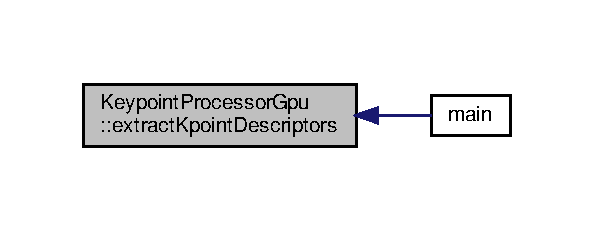
\includegraphics[width=285pt]{classKeypointProcessorGpu_a927a3d8480e8da505524c354e5c02c83_icgraph}
\end{center}
\end{figure}
\mbox{\Hypertarget{classKeypointProcessorGpu_af195f83c19b58a9fedeb50ac3baaa8b3}\label{classKeypointProcessorGpu_af195f83c19b58a9fedeb50ac3baaa8b3}} 
\index{Keypoint\+Processor\+Gpu@{Keypoint\+Processor\+Gpu}!match\+Kpoints@{match\+Kpoints}}
\index{match\+Kpoints@{match\+Kpoints}!Keypoint\+Processor\+Gpu@{Keypoint\+Processor\+Gpu}}
\subsubsection{\texorpdfstring{match\+Kpoints()}{matchKpoints()}}
{\footnotesize\ttfamily void Keypoint\+Processor\+Gpu\+::match\+Kpoints (\begin{DoxyParamCaption}\item[{std\+::string}]{mpoint\+Strategy = {\ttfamily \char`\"{}FUND\char`\"{}} }\end{DoxyParamCaption})}

Here is the caller graph for this function\+:\nopagebreak
\begin{figure}[H]
\begin{center}
\leavevmode
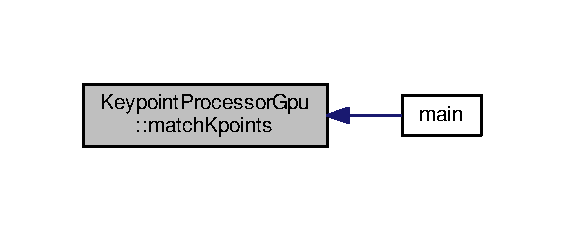
\includegraphics[width=271pt]{classKeypointProcessorGpu_af195f83c19b58a9fedeb50ac3baaa8b3_icgraph}
\end{center}
\end{figure}
\mbox{\Hypertarget{classKeypointProcessorGpu_abdbb860bb800e122dee4c76fcf596fc5}\label{classKeypointProcessorGpu_abdbb860bb800e122dee4c76fcf596fc5}} 
\index{Keypoint\+Processor\+Gpu@{Keypoint\+Processor\+Gpu}!refine\+Matches@{refine\+Matches}}
\index{refine\+Matches@{refine\+Matches}!Keypoint\+Processor\+Gpu@{Keypoint\+Processor\+Gpu}}
\subsubsection{\texorpdfstring{refine\+Matches()}{refineMatches()}}
{\footnotesize\ttfamily \hyperlink{namespaceRefineReturnCode_a54e2cd5f4af90ff2df55bf63455d1959}{Refine\+Return\+Code\+::\+Refine\+Return\+Code} Keypoint\+Processor\+Gpu\+::refine\+Matches (\begin{DoxyParamCaption}\item[{const std\+::vector$<$ cv\+::\+D\+Match $>$ \&}]{matches,  }\item[{std\+::vector$<$ cv\+::\+Key\+Point $>$ \&}]{keypoints1,  }\item[{std\+::vector$<$ cv\+::\+Key\+Point $>$ \&}]{keypoints2,  }\item[{std\+::vector$<$ cv\+::\+D\+Match $>$ \&}]{out\+Matches,  }\item[{std\+::string}]{match\+Refine\+Strategy }\end{DoxyParamCaption})}

\mbox{\Hypertarget{classKeypointProcessorGpu_a192bc98425b2bc0bea56ae024d9584b3}\label{classKeypointProcessorGpu_a192bc98425b2bc0bea56ae024d9584b3}} 
\index{Keypoint\+Processor\+Gpu@{Keypoint\+Processor\+Gpu}!visualize@{visualize}}
\index{visualize@{visualize}!Keypoint\+Processor\+Gpu@{Keypoint\+Processor\+Gpu}}
\subsubsection{\texorpdfstring{visualize()}{visualize()}}
{\footnotesize\ttfamily void Keypoint\+Processor\+Gpu\+::visualize (\begin{DoxyParamCaption}\item[{double}]{wait\+\_\+u\+Sec }\end{DoxyParamCaption})}



\subsection{Member Data Documentation}
\mbox{\Hypertarget{classKeypointProcessorGpu_a042507c38ba05d0987aef504de3b4542}\label{classKeypointProcessorGpu_a042507c38ba05d0987aef504de3b4542}} 
\index{Keypoint\+Processor\+Gpu@{Keypoint\+Processor\+Gpu}!m\+\_\+calc\+Rel\+Vert\+Disp@{m\+\_\+calc\+Rel\+Vert\+Disp}}
\index{m\+\_\+calc\+Rel\+Vert\+Disp@{m\+\_\+calc\+Rel\+Vert\+Disp}!Keypoint\+Processor\+Gpu@{Keypoint\+Processor\+Gpu}}
\subsubsection{\texorpdfstring{m\+\_\+calc\+Rel\+Vert\+Disp}{m\_calcRelVertDisp}}
{\footnotesize\ttfamily bool Keypoint\+Processor\+Gpu\+::m\+\_\+calc\+Rel\+Vert\+Disp = false\hspace{0.3cm}{\ttfamily [private]}}

\mbox{\Hypertarget{classKeypointProcessorGpu_a2630dc84058b86cf55b451457223636c}\label{classKeypointProcessorGpu_a2630dc84058b86cf55b451457223636c}} 
\index{Keypoint\+Processor\+Gpu@{Keypoint\+Processor\+Gpu}!m\+\_\+data\+Frame\+Buffer@{m\+\_\+data\+Frame\+Buffer}}
\index{m\+\_\+data\+Frame\+Buffer@{m\+\_\+data\+Frame\+Buffer}!Keypoint\+Processor\+Gpu@{Keypoint\+Processor\+Gpu}}
\subsubsection{\texorpdfstring{m\+\_\+data\+Frame\+Buffer}{m\_dataFrameBuffer}}
{\footnotesize\ttfamily boost\+::circular\+\_\+buffer$<$\hyperlink{structDataFrame}{Data\+Frame}$>$\& Keypoint\+Processor\+Gpu\+::m\+\_\+data\+Frame\+Buffer\hspace{0.3cm}{\ttfamily [private]}}

\mbox{\Hypertarget{classKeypointProcessorGpu_acc2e8a31a5b2f2e6e4bb491770631935}\label{classKeypointProcessorGpu_acc2e8a31a5b2f2e6e4bb491770631935}} 
\index{Keypoint\+Processor\+Gpu@{Keypoint\+Processor\+Gpu}!m\+\_\+detector\+Type@{m\+\_\+detector\+Type}}
\index{m\+\_\+detector\+Type@{m\+\_\+detector\+Type}!Keypoint\+Processor\+Gpu@{Keypoint\+Processor\+Gpu}}
\subsubsection{\texorpdfstring{m\+\_\+detector\+Type}{m\_detectorType}}
{\footnotesize\ttfamily std\+::string Keypoint\+Processor\+Gpu\+::m\+\_\+detector\+Type\hspace{0.3cm}{\ttfamily [private]}}

\mbox{\Hypertarget{classKeypointProcessorGpu_ae37e6c6a36df9bd6fa3eb8ab0f19e7ee}\label{classKeypointProcessorGpu_ae37e6c6a36df9bd6fa3eb8ab0f19e7ee}} 
\index{Keypoint\+Processor\+Gpu@{Keypoint\+Processor\+Gpu}!m\+\_\+dist\+To\+Epip\+Line@{m\+\_\+dist\+To\+Epip\+Line}}
\index{m\+\_\+dist\+To\+Epip\+Line@{m\+\_\+dist\+To\+Epip\+Line}!Keypoint\+Processor\+Gpu@{Keypoint\+Processor\+Gpu}}
\subsubsection{\texorpdfstring{m\+\_\+dist\+To\+Epip\+Line}{m\_distToEpipLine}}
{\footnotesize\ttfamily double Keypoint\+Processor\+Gpu\+::m\+\_\+dist\+To\+Epip\+Line = 1.\+0\hspace{0.3cm}{\ttfamily [private]}}

\mbox{\Hypertarget{classKeypointProcessorGpu_a2c3270837954025c6dd795cba7ff98f4}\label{classKeypointProcessorGpu_a2c3270837954025c6dd795cba7ff98f4}} 
\index{Keypoint\+Processor\+Gpu@{Keypoint\+Processor\+Gpu}!m\+\_\+fund\+Matrix@{m\+\_\+fund\+Matrix}}
\index{m\+\_\+fund\+Matrix@{m\+\_\+fund\+Matrix}!Keypoint\+Processor\+Gpu@{Keypoint\+Processor\+Gpu}}
\subsubsection{\texorpdfstring{m\+\_\+fund\+Matrix}{m\_fundMatrix}}
{\footnotesize\ttfamily cv\+::\+Mat Keypoint\+Processor\+Gpu\+::m\+\_\+fund\+Matrix\hspace{0.3cm}{\ttfamily [private]}}

\mbox{\Hypertarget{classKeypointProcessorGpu_a7e08f5f64a286910479ec783ed42c810}\label{classKeypointProcessorGpu_a7e08f5f64a286910479ec783ed42c810}} 
\index{Keypoint\+Processor\+Gpu@{Keypoint\+Processor\+Gpu}!m\+\_\+homography\+Matrix@{m\+\_\+homography\+Matrix}}
\index{m\+\_\+homography\+Matrix@{m\+\_\+homography\+Matrix}!Keypoint\+Processor\+Gpu@{Keypoint\+Processor\+Gpu}}
\subsubsection{\texorpdfstring{m\+\_\+homography\+Matrix}{m\_homographyMatrix}}
{\footnotesize\ttfamily cv\+::\+Mat Keypoint\+Processor\+Gpu\+::m\+\_\+homography\+Matrix\hspace{0.3cm}{\ttfamily [private]}}

\mbox{\Hypertarget{classKeypointProcessorGpu_ab610f6f103d888b7c554327a76d58de8}\label{classKeypointProcessorGpu_ab610f6f103d888b7c554327a76d58de8}} 
\index{Keypoint\+Processor\+Gpu@{Keypoint\+Processor\+Gpu}!m\+\_\+ransac\+Confid@{m\+\_\+ransac\+Confid}}
\index{m\+\_\+ransac\+Confid@{m\+\_\+ransac\+Confid}!Keypoint\+Processor\+Gpu@{Keypoint\+Processor\+Gpu}}
\subsubsection{\texorpdfstring{m\+\_\+ransac\+Confid}{m\_ransacConfid}}
{\footnotesize\ttfamily double Keypoint\+Processor\+Gpu\+::m\+\_\+ransac\+Confid = 0.\+9\hspace{0.3cm}{\ttfamily [private]}}

\mbox{\Hypertarget{classKeypointProcessorGpu_ab62f73737e0d61bfc188b23ef4311b63}\label{classKeypointProcessorGpu_ab62f73737e0d61bfc188b23ef4311b63}} 
\index{Keypoint\+Processor\+Gpu@{Keypoint\+Processor\+Gpu}!m\+\_\+refine\+Fund@{m\+\_\+refine\+Fund}}
\index{m\+\_\+refine\+Fund@{m\+\_\+refine\+Fund}!Keypoint\+Processor\+Gpu@{Keypoint\+Processor\+Gpu}}
\subsubsection{\texorpdfstring{m\+\_\+refine\+Fund}{m\_refineFund}}
{\footnotesize\ttfamily bool Keypoint\+Processor\+Gpu\+::m\+\_\+refine\+Fund = true\hspace{0.3cm}{\ttfamily [private]}}

\mbox{\Hypertarget{classKeypointProcessorGpu_a4d74380d0d8a32d06ceb61787c3fb7c5}\label{classKeypointProcessorGpu_a4d74380d0d8a32d06ceb61787c3fb7c5}} 
\index{Keypoint\+Processor\+Gpu@{Keypoint\+Processor\+Gpu}!m\+\_\+refine\+Matches@{m\+\_\+refine\+Matches}}
\index{m\+\_\+refine\+Matches@{m\+\_\+refine\+Matches}!Keypoint\+Processor\+Gpu@{Keypoint\+Processor\+Gpu}}
\subsubsection{\texorpdfstring{m\+\_\+refine\+Matches}{m\_refineMatches}}
{\footnotesize\ttfamily bool Keypoint\+Processor\+Gpu\+::m\+\_\+refine\+Matches = true\hspace{0.3cm}{\ttfamily [private]}}

\mbox{\Hypertarget{classKeypointProcessorGpu_a5f611760beb6ba345fac1eaaccdc3cbe}\label{classKeypointProcessorGpu_a5f611760beb6ba345fac1eaaccdc3cbe}} 
\index{Keypoint\+Processor\+Gpu@{Keypoint\+Processor\+Gpu}!m\+\_\+selector\+Type@{m\+\_\+selector\+Type}}
\index{m\+\_\+selector\+Type@{m\+\_\+selector\+Type}!Keypoint\+Processor\+Gpu@{Keypoint\+Processor\+Gpu}}
\subsubsection{\texorpdfstring{m\+\_\+selector\+Type}{m\_selectorType}}
{\footnotesize\ttfamily std\+::string Keypoint\+Processor\+Gpu\+::m\+\_\+selector\+Type\hspace{0.3cm}{\ttfamily [private]}}

\mbox{\Hypertarget{classKeypointProcessorGpu_a9d5efa15a005d4a2e4c388fa985b93e4}\label{classKeypointProcessorGpu_a9d5efa15a005d4a2e4c388fa985b93e4}} 
\index{Keypoint\+Processor\+Gpu@{Keypoint\+Processor\+Gpu}!m\+\_\+use\+G\+P\+Us@{m\+\_\+use\+G\+P\+Us}}
\index{m\+\_\+use\+G\+P\+Us@{m\+\_\+use\+G\+P\+Us}!Keypoint\+Processor\+Gpu@{Keypoint\+Processor\+Gpu}}
\subsubsection{\texorpdfstring{m\+\_\+use\+G\+P\+Us}{m\_useGPUs}}
{\footnotesize\ttfamily bool Keypoint\+Processor\+Gpu\+::m\+\_\+use\+G\+P\+Us\hspace{0.3cm}{\ttfamily [private]}}

\mbox{\Hypertarget{classKeypointProcessorGpu_a31a0d88cbd1aec736eb30e97413b9247}\label{classKeypointProcessorGpu_a31a0d88cbd1aec736eb30e97413b9247}} 
\index{Keypoint\+Processor\+Gpu@{Keypoint\+Processor\+Gpu}!m\+\_\+visu\+Enable@{m\+\_\+visu\+Enable}}
\index{m\+\_\+visu\+Enable@{m\+\_\+visu\+Enable}!Keypoint\+Processor\+Gpu@{Keypoint\+Processor\+Gpu}}
\subsubsection{\texorpdfstring{m\+\_\+visu\+Enable}{m\_visuEnable}}
{\footnotesize\ttfamily bool Keypoint\+Processor\+Gpu\+::m\+\_\+visu\+Enable\hspace{0.3cm}{\ttfamily [private]}}

\mbox{\Hypertarget{classKeypointProcessorGpu_a298b81730df9cce6b59b0fc35ba1c865}\label{classKeypointProcessorGpu_a298b81730df9cce6b59b0fc35ba1c865}} 
\index{Keypoint\+Processor\+Gpu@{Keypoint\+Processor\+Gpu}!previous\+Frame\+Sts@{previous\+Frame\+Sts}}
\index{previous\+Frame\+Sts@{previous\+Frame\+Sts}!Keypoint\+Processor\+Gpu@{Keypoint\+Processor\+Gpu}}
\subsubsection{\texorpdfstring{previous\+Frame\+Sts}{previousFrameSts}}
{\footnotesize\ttfamily \hyperlink{namespaceFrameSTS_aa00e1583f3bc837ad3fbfb9beaaa0692}{Frame\+S\+T\+S\+::\+Frame\+S\+TS} Keypoint\+Processor\+Gpu\+::previous\+Frame\+Sts = \hyperlink{namespaceFrameSTS_aa00e1583f3bc837ad3fbfb9beaaa0692a8320d47ecf7adbfb6dedd682bf1820db}{Frame\+S\+T\+S\+::\+N\+O\+T\+\_\+\+Y\+E\+T\+\_\+\+P\+R\+O\+C\+E\+S\+S\+ED}\hspace{0.3cm}{\ttfamily [private]}}



The documentation for this class was generated from the following files\+:\begin{DoxyCompactItemize}
\item 
src/pose/\hyperlink{KeypointProcessorGpu_8hpp}{Keypoint\+Processor\+Gpu.\+hpp}\item 
src/pose/\hyperlink{KeypointProcessorGpu_8cpp}{Keypoint\+Processor\+Gpu.\+cpp}\end{DoxyCompactItemize}

\hypertarget{classkpproc_1_1KpointExtractor}{}\section{kpproc\+:\+:Kpoint\+Extractor Class Reference}
\label{classkpproc_1_1KpointExtractor}\index{kpproc\+::\+Kpoint\+Extractor@{kpproc\+::\+Kpoint\+Extractor}}


{\ttfamily \#include $<$Kpoint\+Extractor.\+hpp$>$}

\subsection*{Public Member Functions}
\begin{DoxyCompactItemize}
\item 
\hyperlink{classkpproc_1_1KpointExtractor_ad05a95e4da00ee5d14a4c1b99141cd08}{Kpoint\+Extractor} (bool visu\+Enable=false)
\begin{DoxyCompactList}\small\item\em Keypoint extractor constructor. \end{DoxyCompactList}\item 
bool \hyperlink{classkpproc_1_1KpointExtractor_ade1efa4e540390775ed7158f57ca9618}{extract\+Kpoint\+Descriptors} (const cv\+::\+Mat \&input\+Image)
\begin{DoxyCompactList}\small\item\em This functions detect keypoints and generate descriptors. \end{DoxyCompactList}\item 
void \hyperlink{classkpproc_1_1KpointExtractor_a167e3596663206cb24e9eefe54baf4be}{get\+Results} (std\+::vector$<$ cv\+::\+Key\+Point $>$ \&res\+Keypoints, cv\+::\+Mat \&res\+Descriptors)
\begin{DoxyCompactList}\small\item\em This function retrieve keypoints and their descriptors. \end{DoxyCompactList}\item 
void \hyperlink{classkpproc_1_1KpointExtractor_a52e3033d4c95115f76315c228d3a1350}{visualize} (double wait\+\_\+u\+Sec)
\begin{DoxyCompactList}\small\item\em To visualize keypoints -\/ N\+OT I\+M\+P\+L\+E\+M\+E\+N\+T\+ED. \end{DoxyCompactList}\end{DoxyCompactItemize}
\subsection*{Public Attributes}
\begin{DoxyCompactItemize}
\item 
cv\+::\+Mat \hyperlink{classkpproc_1_1KpointExtractor_ac03e195051022be4aab2a008d05475c4}{m\+\_\+frame\+Img}
\end{DoxyCompactItemize}
\subsection*{Static Public Attributes}
\begin{DoxyCompactItemize}
\item 
static const unsigned int \hyperlink{classkpproc_1_1KpointExtractor_a1d7c3437fc6b2cff35d60df9f554dd12}{M\+I\+N\+\_\+\+K\+P\+O\+I\+N\+T\+\_\+\+N\+BR} = 35
\end{DoxyCompactItemize}
\subsection*{Private Attributes}
\begin{DoxyCompactItemize}
\item 
bool \hyperlink{classkpproc_1_1KpointExtractor_ab0f534203a246814b163aa3dffeef1b5}{m\+\_\+visu\+Enable}
\item 
std\+::vector$<$ cv\+::\+Key\+Point $>$ \hyperlink{classkpproc_1_1KpointExtractor_ace5a9a7c0bc1cea6e181b72f41588205}{m\+\_\+keypoints}
\item 
cv\+::\+Mat \hyperlink{classkpproc_1_1KpointExtractor_a27bff1246cd947b3d84272a4b06b6498}{m\+\_\+descriptors}
\end{DoxyCompactItemize}


\subsection{Detailed Description}
Keypoint extraction class\+: given an image it extracts the keypoints and provide the corresponding descriptors 

\subsection{Constructor \& Destructor Documentation}
\index{kpproc\+::\+Kpoint\+Extractor@{kpproc\+::\+Kpoint\+Extractor}!Kpoint\+Extractor@{Kpoint\+Extractor}}
\index{Kpoint\+Extractor@{Kpoint\+Extractor}!kpproc\+::\+Kpoint\+Extractor@{kpproc\+::\+Kpoint\+Extractor}}
\subsubsection[{\texorpdfstring{Kpoint\+Extractor(bool visu\+Enable=false)}{KpointExtractor(bool visuEnable=false)}}]{\setlength{\rightskip}{0pt plus 5cm}kpproc\+::\+Kpoint\+Extractor\+::\+Kpoint\+Extractor (
\begin{DoxyParamCaption}
\item[{bool}]{visu\+Enable = {\ttfamily false}}
\end{DoxyParamCaption}
)\hspace{0.3cm}{\ttfamily [inline]}}\hypertarget{classkpproc_1_1KpointExtractor_ad05a95e4da00ee5d14a4c1b99141cd08}{}\label{classkpproc_1_1KpointExtractor_ad05a95e4da00ee5d14a4c1b99141cd08}


Keypoint extractor constructor. 


\begin{DoxyParams}{Parameters}
{\em visu\+Enable} & enable/disable keypoints visualization \\
\hline
\end{DoxyParams}


Here is the call graph for this function\+:\nopagebreak
\begin{figure}[H]
\begin{center}
\leavevmode
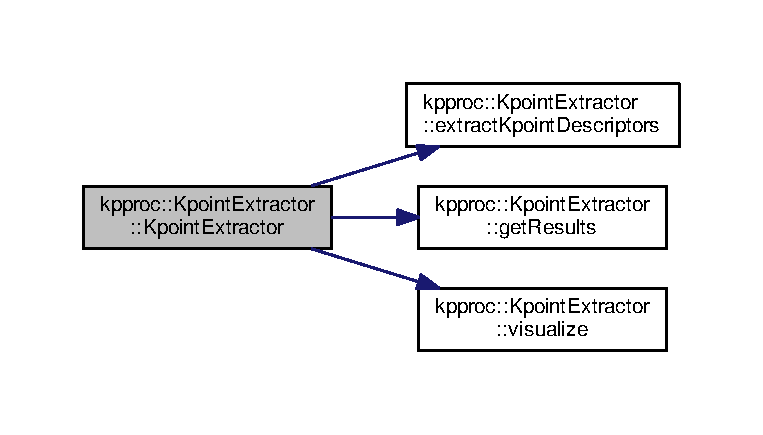
\includegraphics[width=350pt]{classkpproc_1_1KpointExtractor_ad05a95e4da00ee5d14a4c1b99141cd08_cgraph}
\end{center}
\end{figure}




\subsection{Member Function Documentation}
\index{kpproc\+::\+Kpoint\+Extractor@{kpproc\+::\+Kpoint\+Extractor}!extract\+Kpoint\+Descriptors@{extract\+Kpoint\+Descriptors}}
\index{extract\+Kpoint\+Descriptors@{extract\+Kpoint\+Descriptors}!kpproc\+::\+Kpoint\+Extractor@{kpproc\+::\+Kpoint\+Extractor}}
\subsubsection[{\texorpdfstring{extract\+Kpoint\+Descriptors(const cv\+::\+Mat \&input\+Image)}{extractKpointDescriptors(const cv::Mat &inputImage)}}]{\setlength{\rightskip}{0pt plus 5cm}bool Kpoint\+Extractor\+::extract\+Kpoint\+Descriptors (
\begin{DoxyParamCaption}
\item[{const cv\+::\+Mat \&}]{input\+Image}
\end{DoxyParamCaption}
)}\hypertarget{classkpproc_1_1KpointExtractor_ade1efa4e540390775ed7158f57ca9618}{}\label{classkpproc_1_1KpointExtractor_ade1efa4e540390775ed7158f57ca9618}


This functions detect keypoints and generate descriptors. 


\begin{DoxyParams}{Parameters}
{\em input\+Image} & The image where the keypoints will be extracted from\\
\hline
\end{DoxyParams}
\begin{DoxyReturn}{Returns}
true on success. 
\end{DoxyReturn}


Here is the caller graph for this function\+:\nopagebreak
\begin{figure}[H]
\begin{center}
\leavevmode
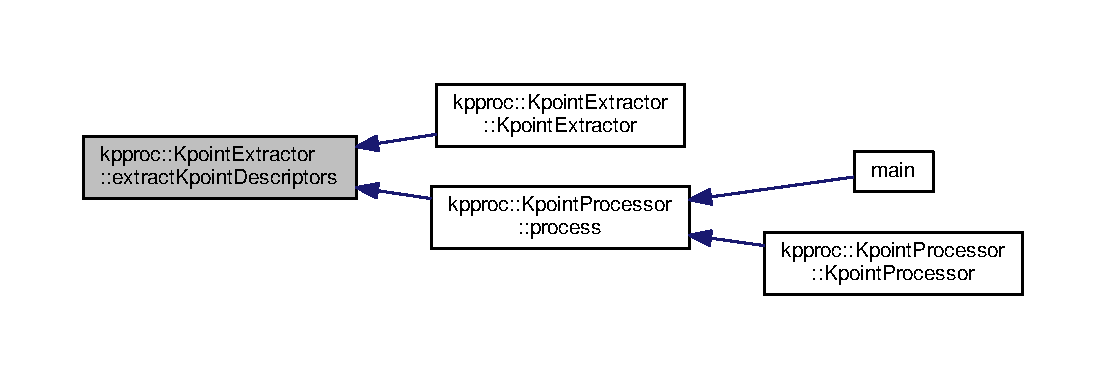
\includegraphics[width=350pt]{classkpproc_1_1KpointExtractor_ade1efa4e540390775ed7158f57ca9618_icgraph}
\end{center}
\end{figure}


\index{kpproc\+::\+Kpoint\+Extractor@{kpproc\+::\+Kpoint\+Extractor}!get\+Results@{get\+Results}}
\index{get\+Results@{get\+Results}!kpproc\+::\+Kpoint\+Extractor@{kpproc\+::\+Kpoint\+Extractor}}
\subsubsection[{\texorpdfstring{get\+Results(std\+::vector$<$ cv\+::\+Key\+Point $>$ \&res\+Keypoints, cv\+::\+Mat \&res\+Descriptors)}{getResults(std::vector< cv::KeyPoint > &resKeypoints, cv::Mat &resDescriptors)}}]{\setlength{\rightskip}{0pt plus 5cm}void Kpoint\+Extractor\+::get\+Results (
\begin{DoxyParamCaption}
\item[{std\+::vector$<$ cv\+::\+Key\+Point $>$ \&}]{res\+Keypoints, }
\item[{cv\+::\+Mat \&}]{res\+Descriptors}
\end{DoxyParamCaption}
)}\hypertarget{classkpproc_1_1KpointExtractor_a167e3596663206cb24e9eefe54baf4be}{}\label{classkpproc_1_1KpointExtractor_a167e3596663206cb24e9eefe54baf4be}


This function retrieve keypoints and their descriptors. 


\begin{DoxyParams}{Parameters}
{\em res\+Keypoints} & where the keypoints will be stored \\
\hline
{\em res\+Descriptors} & where the descriptors will be stored\\
\hline
\end{DoxyParams}
\begin{DoxyReturn}{Returns}
true on success. 
\end{DoxyReturn}


Here is the caller graph for this function\+:\nopagebreak
\begin{figure}[H]
\begin{center}
\leavevmode
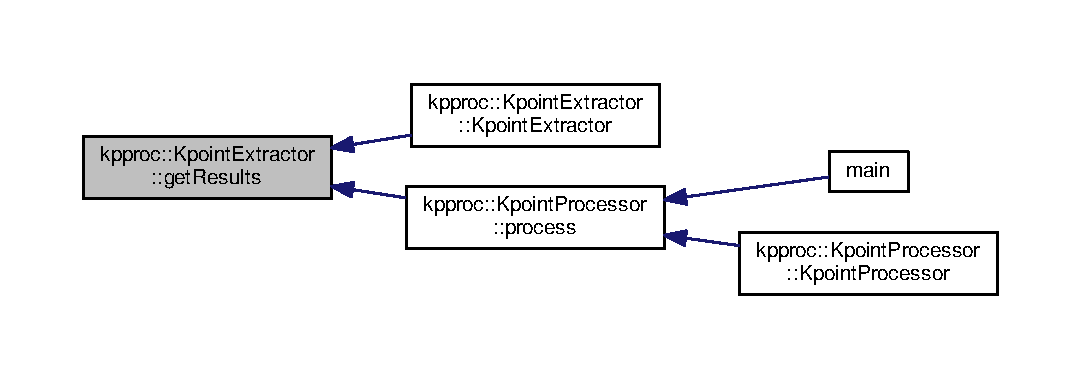
\includegraphics[width=350pt]{classkpproc_1_1KpointExtractor_a167e3596663206cb24e9eefe54baf4be_icgraph}
\end{center}
\end{figure}


\index{kpproc\+::\+Kpoint\+Extractor@{kpproc\+::\+Kpoint\+Extractor}!visualize@{visualize}}
\index{visualize@{visualize}!kpproc\+::\+Kpoint\+Extractor@{kpproc\+::\+Kpoint\+Extractor}}
\subsubsection[{\texorpdfstring{visualize(double wait\+\_\+u\+Sec)}{visualize(double wait_uSec)}}]{\setlength{\rightskip}{0pt plus 5cm}void kpproc\+::\+Kpoint\+Extractor\+::visualize (
\begin{DoxyParamCaption}
\item[{double}]{wait\+\_\+u\+Sec}
\end{DoxyParamCaption}
)}\hypertarget{classkpproc_1_1KpointExtractor_a52e3033d4c95115f76315c228d3a1350}{}\label{classkpproc_1_1KpointExtractor_a52e3033d4c95115f76315c228d3a1350}


To visualize keypoints -\/ N\+OT I\+M\+P\+L\+E\+M\+E\+N\+T\+ED. 

\begin{DoxyReturn}{Returns}
void. 
\end{DoxyReturn}


Here is the caller graph for this function\+:\nopagebreak
\begin{figure}[H]
\begin{center}
\leavevmode
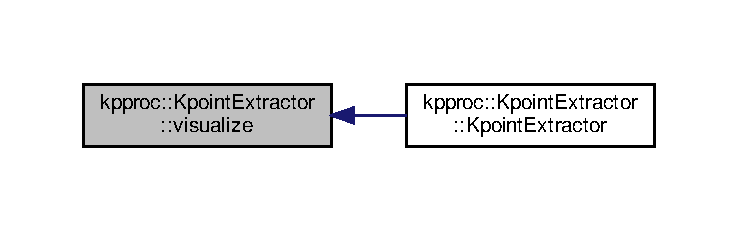
\includegraphics[width=350pt]{classkpproc_1_1KpointExtractor_a52e3033d4c95115f76315c228d3a1350_icgraph}
\end{center}
\end{figure}




\subsection{Member Data Documentation}
\index{kpproc\+::\+Kpoint\+Extractor@{kpproc\+::\+Kpoint\+Extractor}!m\+\_\+descriptors@{m\+\_\+descriptors}}
\index{m\+\_\+descriptors@{m\+\_\+descriptors}!kpproc\+::\+Kpoint\+Extractor@{kpproc\+::\+Kpoint\+Extractor}}
\subsubsection[{\texorpdfstring{m\+\_\+descriptors}{m_descriptors}}]{\setlength{\rightskip}{0pt plus 5cm}cv\+::\+Mat kpproc\+::\+Kpoint\+Extractor\+::m\+\_\+descriptors\hspace{0.3cm}{\ttfamily [private]}}\hypertarget{classkpproc_1_1KpointExtractor_a27bff1246cd947b3d84272a4b06b6498}{}\label{classkpproc_1_1KpointExtractor_a27bff1246cd947b3d84272a4b06b6498}
keypoint descriptors associated to keypoints listed in \hyperlink{classkpproc_1_1KpointExtractor_ace5a9a7c0bc1cea6e181b72f41588205}{m\+\_\+keypoints} \index{kpproc\+::\+Kpoint\+Extractor@{kpproc\+::\+Kpoint\+Extractor}!m\+\_\+frame\+Img@{m\+\_\+frame\+Img}}
\index{m\+\_\+frame\+Img@{m\+\_\+frame\+Img}!kpproc\+::\+Kpoint\+Extractor@{kpproc\+::\+Kpoint\+Extractor}}
\subsubsection[{\texorpdfstring{m\+\_\+frame\+Img}{m_frameImg}}]{\setlength{\rightskip}{0pt plus 5cm}cv\+::\+Mat kpproc\+::\+Kpoint\+Extractor\+::m\+\_\+frame\+Img}\hypertarget{classkpproc_1_1KpointExtractor_ac03e195051022be4aab2a008d05475c4}{}\label{classkpproc_1_1KpointExtractor_ac03e195051022be4aab2a008d05475c4}
The image of this frame in cv\+::\+Mat format \index{kpproc\+::\+Kpoint\+Extractor@{kpproc\+::\+Kpoint\+Extractor}!m\+\_\+keypoints@{m\+\_\+keypoints}}
\index{m\+\_\+keypoints@{m\+\_\+keypoints}!kpproc\+::\+Kpoint\+Extractor@{kpproc\+::\+Kpoint\+Extractor}}
\subsubsection[{\texorpdfstring{m\+\_\+keypoints}{m_keypoints}}]{\setlength{\rightskip}{0pt plus 5cm}std\+::vector$<$cv\+::\+Key\+Point$>$ kpproc\+::\+Kpoint\+Extractor\+::m\+\_\+keypoints\hspace{0.3cm}{\ttfamily [private]}}\hypertarget{classkpproc_1_1KpointExtractor_ace5a9a7c0bc1cea6e181b72f41588205}{}\label{classkpproc_1_1KpointExtractor_ace5a9a7c0bc1cea6e181b72f41588205}
Keypoints within camera image \index{kpproc\+::\+Kpoint\+Extractor@{kpproc\+::\+Kpoint\+Extractor}!m\+\_\+visu\+Enable@{m\+\_\+visu\+Enable}}
\index{m\+\_\+visu\+Enable@{m\+\_\+visu\+Enable}!kpproc\+::\+Kpoint\+Extractor@{kpproc\+::\+Kpoint\+Extractor}}
\subsubsection[{\texorpdfstring{m\+\_\+visu\+Enable}{m_visuEnable}}]{\setlength{\rightskip}{0pt plus 5cm}bool kpproc\+::\+Kpoint\+Extractor\+::m\+\_\+visu\+Enable\hspace{0.3cm}{\ttfamily [private]}}\hypertarget{classkpproc_1_1KpointExtractor_ab0f534203a246814b163aa3dffeef1b5}{}\label{classkpproc_1_1KpointExtractor_ab0f534203a246814b163aa3dffeef1b5}
To store visualization enable or disable status \index{kpproc\+::\+Kpoint\+Extractor@{kpproc\+::\+Kpoint\+Extractor}!M\+I\+N\+\_\+\+K\+P\+O\+I\+N\+T\+\_\+\+N\+BR@{M\+I\+N\+\_\+\+K\+P\+O\+I\+N\+T\+\_\+\+N\+BR}}
\index{M\+I\+N\+\_\+\+K\+P\+O\+I\+N\+T\+\_\+\+N\+BR@{M\+I\+N\+\_\+\+K\+P\+O\+I\+N\+T\+\_\+\+N\+BR}!kpproc\+::\+Kpoint\+Extractor@{kpproc\+::\+Kpoint\+Extractor}}
\subsubsection[{\texorpdfstring{M\+I\+N\+\_\+\+K\+P\+O\+I\+N\+T\+\_\+\+N\+BR}{MIN_KPOINT_NBR}}]{\setlength{\rightskip}{0pt plus 5cm}const unsigned int kpproc\+::\+Kpoint\+Extractor\+::\+M\+I\+N\+\_\+\+K\+P\+O\+I\+N\+T\+\_\+\+N\+BR = 35\hspace{0.3cm}{\ttfamily [static]}}\hypertarget{classkpproc_1_1KpointExtractor_a1d7c3437fc6b2cff35d60df9f554dd12}{}\label{classkpproc_1_1KpointExtractor_a1d7c3437fc6b2cff35d60df9f554dd12}
Minimum number of keypoints to consider this frame or image is useful 

The documentation for this class was generated from the following files\+:\begin{DoxyCompactItemize}
\item 
src/pose/\hyperlink{KpointExtractor_8hpp}{Kpoint\+Extractor.\+hpp}\item 
src/pose/\hyperlink{KpointExtractor_8cpp}{Kpoint\+Extractor.\+cpp}\end{DoxyCompactItemize}

\hypertarget{classkpproc_1_1KpointMatcher}{}\section{kpproc\+:\+:Kpoint\+Matcher Class Reference}
\label{classkpproc_1_1KpointMatcher}\index{kpproc\+::\+Kpoint\+Matcher@{kpproc\+::\+Kpoint\+Matcher}}


{\ttfamily \#include $<$Kpoint\+Matcher.\+hpp$>$}

\subsection*{Public Member Functions}
\begin{DoxyCompactItemize}
\item 
\hyperlink{classkpproc_1_1KpointMatcher_a4a40c73477a60c38e5f12ed6f204ab9a}{Kpoint\+Matcher} ()
\item 
bool \hyperlink{classkpproc_1_1KpointMatcher_a21caea2a00576784b2fc90dd652870ed}{match} (const cv\+::\+Mat \&query\+Descriptors, const cv\+::\+Mat \&train\+Descriptors, const std\+::vector$<$ cv\+::\+Key\+Point $>$ \&query\+Keypoints, const std\+::vector$<$ cv\+::\+Key\+Point $>$ \&train\+Keypoints)
\item 
void \hyperlink{classkpproc_1_1KpointMatcher_a02f6944a8401a2a14bb5ce42073389b0}{get\+Results} (std\+::vector$<$ cv\+::\+D\+Match $>$ \&matches, std\+::vector$<$ cv\+::\+Point2f $>$ \&refined\+Points\+Prev, std\+::vector$<$ cv\+::\+Point2f $>$ \&refined\+Points\+Curr)
\end{DoxyCompactItemize}
\subsection*{Public Attributes}
\begin{DoxyCompactItemize}
\item 
std\+::vector$<$ cv\+::\+D\+Match $>$ \hyperlink{classkpproc_1_1KpointMatcher_a082b2988b8e0381f2286dcaa1725a8db}{m\+\_\+matches}
\item 
std\+::vector$<$ cv\+::\+Point2f $>$ \hyperlink{classkpproc_1_1KpointMatcher_a9a0c678dccf356d72b2a69542bcfe960}{m\+\_\+refined\+Points\+Curr}
\item 
std\+::vector$<$ cv\+::\+Point2f $>$ \hyperlink{classkpproc_1_1KpointMatcher_ad21af067c2a5fa339aba9abe85fa943a}{m\+\_\+refined\+Points\+Prev}
\end{DoxyCompactItemize}
\subsection*{Static Public Attributes}
\begin{DoxyCompactItemize}
\item 
static const unsigned int \hyperlink{classkpproc_1_1KpointMatcher_a35b716145fb33b20b3ca2bfec10e343e}{M\+I\+N\+\_\+\+K\+P\+M\+A\+T\+C\+H\+S\+\_\+\+N\+BR} = 16
\item 
static const unsigned int \hyperlink{classkpproc_1_1KpointMatcher_a4d0c0de93ab29378a504265e263663f6}{M\+I\+N\+\_\+\+H\+O\+M\+O\+G\+R\+\_\+\+I\+N\+L\+I\+E\+R\+S\+\_\+\+N\+BR} = 8
\item 
static constexpr double \hyperlink{classkpproc_1_1KpointMatcher_a1efd51083ded96127c34697340e5e92e}{D\+I\+S\+T\+\_\+\+T\+O\+\_\+\+E\+P\+I\+L\+I\+NE} = 3.\+0
\end{DoxyCompactItemize}
\subsection*{Private Member Functions}
\begin{DoxyCompactItemize}
\item 
bool \hyperlink{classkpproc_1_1KpointMatcher_a0d1681f55cfeea8a51bba9ccac41d346}{refine\+Matches} (const cv\+::\+Mat \&query\+Descriptors, const cv\+::\+Mat \&train\+Descriptors, const std\+::vector$<$ cv\+::\+Key\+Point $>$ \&query\+Keypoints, const std\+::vector$<$ cv\+::\+Key\+Point $>$ \&train\+Keypoints, std\+::vector$<$ cv\+::\+D\+Match $>$ \&refined\+Matches)
\end{DoxyCompactItemize}


\subsection{Constructor \& Destructor Documentation}
\mbox{\Hypertarget{classkpproc_1_1KpointMatcher_a4a40c73477a60c38e5f12ed6f204ab9a}\label{classkpproc_1_1KpointMatcher_a4a40c73477a60c38e5f12ed6f204ab9a}} 
\index{kpproc\+::\+Kpoint\+Matcher@{kpproc\+::\+Kpoint\+Matcher}!Kpoint\+Matcher@{Kpoint\+Matcher}}
\index{Kpoint\+Matcher@{Kpoint\+Matcher}!kpproc\+::\+Kpoint\+Matcher@{kpproc\+::\+Kpoint\+Matcher}}
\subsubsection{\texorpdfstring{Kpoint\+Matcher()}{KpointMatcher()}}
{\footnotesize\ttfamily kpproc\+::\+Kpoint\+Matcher\+::\+Kpoint\+Matcher (\begin{DoxyParamCaption}{ }\end{DoxyParamCaption})\hspace{0.3cm}{\ttfamily [inline]}}

Here is the call graph for this function\+:\nopagebreak
\begin{figure}[H]
\begin{center}
\leavevmode
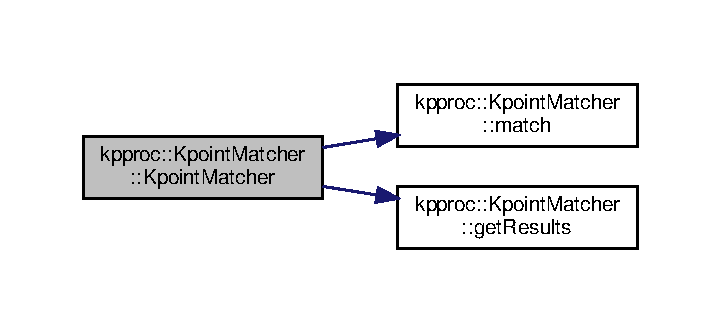
\includegraphics[width=346pt]{classkpproc_1_1KpointMatcher_a4a40c73477a60c38e5f12ed6f204ab9a_cgraph}
\end{center}
\end{figure}


\subsection{Member Function Documentation}
\mbox{\Hypertarget{classkpproc_1_1KpointMatcher_a02f6944a8401a2a14bb5ce42073389b0}\label{classkpproc_1_1KpointMatcher_a02f6944a8401a2a14bb5ce42073389b0}} 
\index{kpproc\+::\+Kpoint\+Matcher@{kpproc\+::\+Kpoint\+Matcher}!get\+Results@{get\+Results}}
\index{get\+Results@{get\+Results}!kpproc\+::\+Kpoint\+Matcher@{kpproc\+::\+Kpoint\+Matcher}}
\subsubsection{\texorpdfstring{get\+Results()}{getResults()}}
{\footnotesize\ttfamily void Kpoint\+Matcher\+::get\+Results (\begin{DoxyParamCaption}\item[{std\+::vector$<$ cv\+::\+D\+Match $>$ \&}]{matches,  }\item[{std\+::vector$<$ cv\+::\+Point2f $>$ \&}]{refined\+Points\+Prev,  }\item[{std\+::vector$<$ cv\+::\+Point2f $>$ \&}]{refined\+Points\+Curr }\end{DoxyParamCaption})}

Here is the caller graph for this function\+:\nopagebreak
\begin{figure}[H]
\begin{center}
\leavevmode
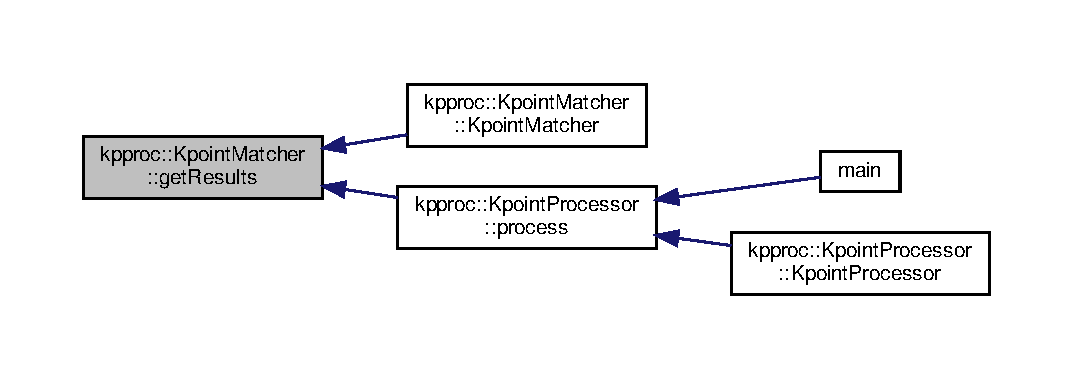
\includegraphics[width=350pt]{classkpproc_1_1KpointMatcher_a02f6944a8401a2a14bb5ce42073389b0_icgraph}
\end{center}
\end{figure}
\mbox{\Hypertarget{classkpproc_1_1KpointMatcher_a21caea2a00576784b2fc90dd652870ed}\label{classkpproc_1_1KpointMatcher_a21caea2a00576784b2fc90dd652870ed}} 
\index{kpproc\+::\+Kpoint\+Matcher@{kpproc\+::\+Kpoint\+Matcher}!match@{match}}
\index{match@{match}!kpproc\+::\+Kpoint\+Matcher@{kpproc\+::\+Kpoint\+Matcher}}
\subsubsection{\texorpdfstring{match()}{match()}}
{\footnotesize\ttfamily bool Kpoint\+Matcher\+::match (\begin{DoxyParamCaption}\item[{const cv\+::\+Mat \&}]{query\+Descriptors,  }\item[{const cv\+::\+Mat \&}]{train\+Descriptors,  }\item[{const std\+::vector$<$ cv\+::\+Key\+Point $>$ \&}]{query\+Keypoints,  }\item[{const std\+::vector$<$ cv\+::\+Key\+Point $>$ \&}]{train\+Keypoints }\end{DoxyParamCaption})}

Here is the caller graph for this function\+:\nopagebreak
\begin{figure}[H]
\begin{center}
\leavevmode
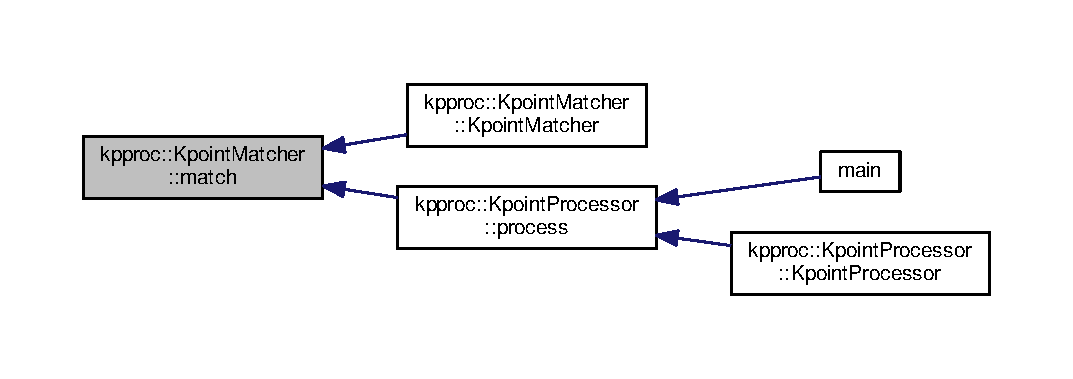
\includegraphics[width=350pt]{classkpproc_1_1KpointMatcher_a21caea2a00576784b2fc90dd652870ed_icgraph}
\end{center}
\end{figure}
\mbox{\Hypertarget{classkpproc_1_1KpointMatcher_a0d1681f55cfeea8a51bba9ccac41d346}\label{classkpproc_1_1KpointMatcher_a0d1681f55cfeea8a51bba9ccac41d346}} 
\index{kpproc\+::\+Kpoint\+Matcher@{kpproc\+::\+Kpoint\+Matcher}!refine\+Matches@{refine\+Matches}}
\index{refine\+Matches@{refine\+Matches}!kpproc\+::\+Kpoint\+Matcher@{kpproc\+::\+Kpoint\+Matcher}}
\subsubsection{\texorpdfstring{refine\+Matches()}{refineMatches()}}
{\footnotesize\ttfamily bool Kpoint\+Matcher\+::refine\+Matches (\begin{DoxyParamCaption}\item[{const cv\+::\+Mat \&}]{query\+Descriptors,  }\item[{const cv\+::\+Mat \&}]{train\+Descriptors,  }\item[{const std\+::vector$<$ cv\+::\+Key\+Point $>$ \&}]{query\+Keypoints,  }\item[{const std\+::vector$<$ cv\+::\+Key\+Point $>$ \&}]{train\+Keypoints,  }\item[{std\+::vector$<$ cv\+::\+D\+Match $>$ \&}]{refined\+Matches }\end{DoxyParamCaption})\hspace{0.3cm}{\ttfamily [private]}}



\subsection{Member Data Documentation}
\mbox{\Hypertarget{classkpproc_1_1KpointMatcher_a1efd51083ded96127c34697340e5e92e}\label{classkpproc_1_1KpointMatcher_a1efd51083ded96127c34697340e5e92e}} 
\index{kpproc\+::\+Kpoint\+Matcher@{kpproc\+::\+Kpoint\+Matcher}!D\+I\+S\+T\+\_\+\+T\+O\+\_\+\+E\+P\+I\+L\+I\+NE@{D\+I\+S\+T\+\_\+\+T\+O\+\_\+\+E\+P\+I\+L\+I\+NE}}
\index{D\+I\+S\+T\+\_\+\+T\+O\+\_\+\+E\+P\+I\+L\+I\+NE@{D\+I\+S\+T\+\_\+\+T\+O\+\_\+\+E\+P\+I\+L\+I\+NE}!kpproc\+::\+Kpoint\+Matcher@{kpproc\+::\+Kpoint\+Matcher}}
\subsubsection{\texorpdfstring{D\+I\+S\+T\+\_\+\+T\+O\+\_\+\+E\+P\+I\+L\+I\+NE}{DIST\_TO\_EPILINE}}
{\footnotesize\ttfamily constexpr double kpproc\+::\+Kpoint\+Matcher\+::\+D\+I\+S\+T\+\_\+\+T\+O\+\_\+\+E\+P\+I\+L\+I\+NE = 3.\+0\hspace{0.3cm}{\ttfamily [static]}}

\mbox{\Hypertarget{classkpproc_1_1KpointMatcher_a082b2988b8e0381f2286dcaa1725a8db}\label{classkpproc_1_1KpointMatcher_a082b2988b8e0381f2286dcaa1725a8db}} 
\index{kpproc\+::\+Kpoint\+Matcher@{kpproc\+::\+Kpoint\+Matcher}!m\+\_\+matches@{m\+\_\+matches}}
\index{m\+\_\+matches@{m\+\_\+matches}!kpproc\+::\+Kpoint\+Matcher@{kpproc\+::\+Kpoint\+Matcher}}
\subsubsection{\texorpdfstring{m\+\_\+matches}{m\_matches}}
{\footnotesize\ttfamily std\+::vector$<$ cv\+::\+D\+Match $>$ kpproc\+::\+Kpoint\+Matcher\+::m\+\_\+matches}

\mbox{\Hypertarget{classkpproc_1_1KpointMatcher_a9a0c678dccf356d72b2a69542bcfe960}\label{classkpproc_1_1KpointMatcher_a9a0c678dccf356d72b2a69542bcfe960}} 
\index{kpproc\+::\+Kpoint\+Matcher@{kpproc\+::\+Kpoint\+Matcher}!m\+\_\+refined\+Points\+Curr@{m\+\_\+refined\+Points\+Curr}}
\index{m\+\_\+refined\+Points\+Curr@{m\+\_\+refined\+Points\+Curr}!kpproc\+::\+Kpoint\+Matcher@{kpproc\+::\+Kpoint\+Matcher}}
\subsubsection{\texorpdfstring{m\+\_\+refined\+Points\+Curr}{m\_refinedPointsCurr}}
{\footnotesize\ttfamily std\+::vector$<$cv\+::\+Point2f$>$ kpproc\+::\+Kpoint\+Matcher\+::m\+\_\+refined\+Points\+Curr}

\mbox{\Hypertarget{classkpproc_1_1KpointMatcher_ad21af067c2a5fa339aba9abe85fa943a}\label{classkpproc_1_1KpointMatcher_ad21af067c2a5fa339aba9abe85fa943a}} 
\index{kpproc\+::\+Kpoint\+Matcher@{kpproc\+::\+Kpoint\+Matcher}!m\+\_\+refined\+Points\+Prev@{m\+\_\+refined\+Points\+Prev}}
\index{m\+\_\+refined\+Points\+Prev@{m\+\_\+refined\+Points\+Prev}!kpproc\+::\+Kpoint\+Matcher@{kpproc\+::\+Kpoint\+Matcher}}
\subsubsection{\texorpdfstring{m\+\_\+refined\+Points\+Prev}{m\_refinedPointsPrev}}
{\footnotesize\ttfamily std\+::vector$<$cv\+::\+Point2f$>$ kpproc\+::\+Kpoint\+Matcher\+::m\+\_\+refined\+Points\+Prev}

\mbox{\Hypertarget{classkpproc_1_1KpointMatcher_a4d0c0de93ab29378a504265e263663f6}\label{classkpproc_1_1KpointMatcher_a4d0c0de93ab29378a504265e263663f6}} 
\index{kpproc\+::\+Kpoint\+Matcher@{kpproc\+::\+Kpoint\+Matcher}!M\+I\+N\+\_\+\+H\+O\+M\+O\+G\+R\+\_\+\+I\+N\+L\+I\+E\+R\+S\+\_\+\+N\+BR@{M\+I\+N\+\_\+\+H\+O\+M\+O\+G\+R\+\_\+\+I\+N\+L\+I\+E\+R\+S\+\_\+\+N\+BR}}
\index{M\+I\+N\+\_\+\+H\+O\+M\+O\+G\+R\+\_\+\+I\+N\+L\+I\+E\+R\+S\+\_\+\+N\+BR@{M\+I\+N\+\_\+\+H\+O\+M\+O\+G\+R\+\_\+\+I\+N\+L\+I\+E\+R\+S\+\_\+\+N\+BR}!kpproc\+::\+Kpoint\+Matcher@{kpproc\+::\+Kpoint\+Matcher}}
\subsubsection{\texorpdfstring{M\+I\+N\+\_\+\+H\+O\+M\+O\+G\+R\+\_\+\+I\+N\+L\+I\+E\+R\+S\+\_\+\+N\+BR}{MIN\_HOMOGR\_INLIERS\_NBR}}
{\footnotesize\ttfamily const unsigned int kpproc\+::\+Kpoint\+Matcher\+::\+M\+I\+N\+\_\+\+H\+O\+M\+O\+G\+R\+\_\+\+I\+N\+L\+I\+E\+R\+S\+\_\+\+N\+BR = 8\hspace{0.3cm}{\ttfamily [static]}}

\mbox{\Hypertarget{classkpproc_1_1KpointMatcher_a35b716145fb33b20b3ca2bfec10e343e}\label{classkpproc_1_1KpointMatcher_a35b716145fb33b20b3ca2bfec10e343e}} 
\index{kpproc\+::\+Kpoint\+Matcher@{kpproc\+::\+Kpoint\+Matcher}!M\+I\+N\+\_\+\+K\+P\+M\+A\+T\+C\+H\+S\+\_\+\+N\+BR@{M\+I\+N\+\_\+\+K\+P\+M\+A\+T\+C\+H\+S\+\_\+\+N\+BR}}
\index{M\+I\+N\+\_\+\+K\+P\+M\+A\+T\+C\+H\+S\+\_\+\+N\+BR@{M\+I\+N\+\_\+\+K\+P\+M\+A\+T\+C\+H\+S\+\_\+\+N\+BR}!kpproc\+::\+Kpoint\+Matcher@{kpproc\+::\+Kpoint\+Matcher}}
\subsubsection{\texorpdfstring{M\+I\+N\+\_\+\+K\+P\+M\+A\+T\+C\+H\+S\+\_\+\+N\+BR}{MIN\_KPMATCHS\_NBR}}
{\footnotesize\ttfamily const unsigned int kpproc\+::\+Kpoint\+Matcher\+::\+M\+I\+N\+\_\+\+K\+P\+M\+A\+T\+C\+H\+S\+\_\+\+N\+BR = 16\hspace{0.3cm}{\ttfamily [static]}}



The documentation for this class was generated from the following files\+:\begin{DoxyCompactItemize}
\item 
src/pose/\hyperlink{KpointMatcher_8hpp}{Kpoint\+Matcher.\+hpp}\item 
src/pose/\hyperlink{KpointMatcher_8cpp}{Kpoint\+Matcher.\+cpp}\end{DoxyCompactItemize}

\hypertarget{classkpproc_1_1KpointProcessor}{}\section{kpproc\+:\+:Kpoint\+Processor Class Reference}
\label{classkpproc_1_1KpointProcessor}\index{kpproc\+::\+Kpoint\+Processor@{kpproc\+::\+Kpoint\+Processor}}


{\ttfamily \#include $<$Kpoint\+Processor.\+hpp$>$}



Collaboration diagram for kpproc\+:\+:Kpoint\+Processor\+:\nopagebreak
\begin{figure}[H]
\begin{center}
\leavevmode
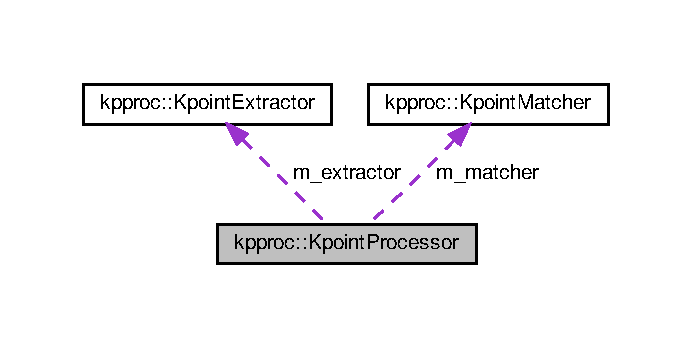
\includegraphics[width=332pt]{classkpproc_1_1KpointProcessor__coll__graph}
\end{center}
\end{figure}
\subsection*{Public Member Functions}
\begin{DoxyCompactItemize}
\item 
\hyperlink{classkpproc_1_1KpointProcessor_a7a10f7352ccb9ab714052144bde69228}{Kpoint\+Processor} (boost\+::circular\+\_\+buffer$<$ \hyperlink{classFrame}{Frame} $>$ \&frame\+Buffer, bool visu\+Enable=false)
\item 
bool \hyperlink{classkpproc_1_1KpointProcessor_a35bdf2239f6742875bbc64338488075a}{process} ()
\end{DoxyCompactItemize}
\subsection*{Public Attributes}
\begin{DoxyCompactItemize}
\item 
\hyperlink{classkpproc_1_1KpointExtractor}{Kpoint\+Extractor} \hyperlink{classkpproc_1_1KpointProcessor_a5ae3277154dd03cddf303d3be6bb37f7}{m\+\_\+extractor}
\item 
\hyperlink{classkpproc_1_1KpointMatcher}{Kpoint\+Matcher} \hyperlink{classkpproc_1_1KpointProcessor_a188352f2093e636cbb06114b4ac7288a}{m\+\_\+matcher}
\item 
boost\+::circular\+\_\+buffer$<$ \hyperlink{classFrame}{Frame} $>$ \& \hyperlink{classkpproc_1_1KpointProcessor_a7faab52da545a233fab6ec061338393e}{m\+\_\+frame\+Buffer}
\end{DoxyCompactItemize}
\subsection*{Private Attributes}
\begin{DoxyCompactItemize}
\item 
bool \hyperlink{classkpproc_1_1KpointProcessor_ac521fd8cfc2400004e729fc504209232}{m\+\_\+visu\+Enable}
\end{DoxyCompactItemize}


\subsection{Constructor \& Destructor Documentation}
\mbox{\Hypertarget{classkpproc_1_1KpointProcessor_a7a10f7352ccb9ab714052144bde69228}\label{classkpproc_1_1KpointProcessor_a7a10f7352ccb9ab714052144bde69228}} 
\index{kpproc\+::\+Kpoint\+Processor@{kpproc\+::\+Kpoint\+Processor}!Kpoint\+Processor@{Kpoint\+Processor}}
\index{Kpoint\+Processor@{Kpoint\+Processor}!kpproc\+::\+Kpoint\+Processor@{kpproc\+::\+Kpoint\+Processor}}
\subsubsection{\texorpdfstring{Kpoint\+Processor()}{KpointProcessor()}}
{\footnotesize\ttfamily kpproc\+::\+Kpoint\+Processor\+::\+Kpoint\+Processor (\begin{DoxyParamCaption}\item[{boost\+::circular\+\_\+buffer$<$ \hyperlink{classFrame}{Frame} $>$ \&}]{frame\+Buffer,  }\item[{bool}]{visu\+Enable = {\ttfamily false} }\end{DoxyParamCaption})\hspace{0.3cm}{\ttfamily [inline]}}

Here is the call graph for this function\+:\nopagebreak
\begin{figure}[H]
\begin{center}
\leavevmode
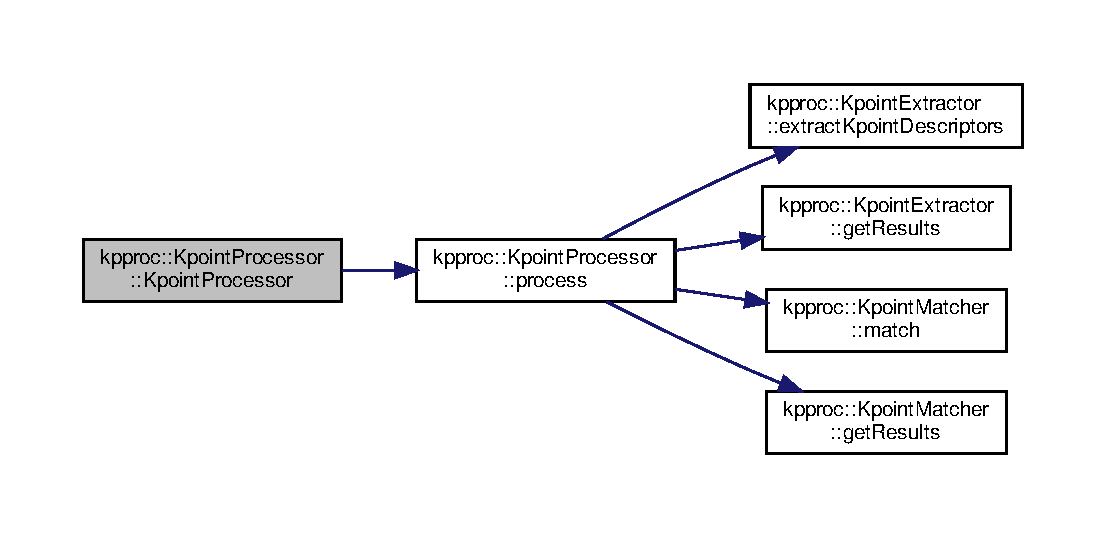
\includegraphics[width=350pt]{classkpproc_1_1KpointProcessor_a7a10f7352ccb9ab714052144bde69228_cgraph}
\end{center}
\end{figure}


\subsection{Member Function Documentation}
\mbox{\Hypertarget{classkpproc_1_1KpointProcessor_a35bdf2239f6742875bbc64338488075a}\label{classkpproc_1_1KpointProcessor_a35bdf2239f6742875bbc64338488075a}} 
\index{kpproc\+::\+Kpoint\+Processor@{kpproc\+::\+Kpoint\+Processor}!process@{process}}
\index{process@{process}!kpproc\+::\+Kpoint\+Processor@{kpproc\+::\+Kpoint\+Processor}}
\subsubsection{\texorpdfstring{process()}{process()}}
{\footnotesize\ttfamily bool Kpoint\+Processor\+::process (\begin{DoxyParamCaption}{ }\end{DoxyParamCaption})}

Here is the call graph for this function\+:\nopagebreak
\begin{figure}[H]
\begin{center}
\leavevmode
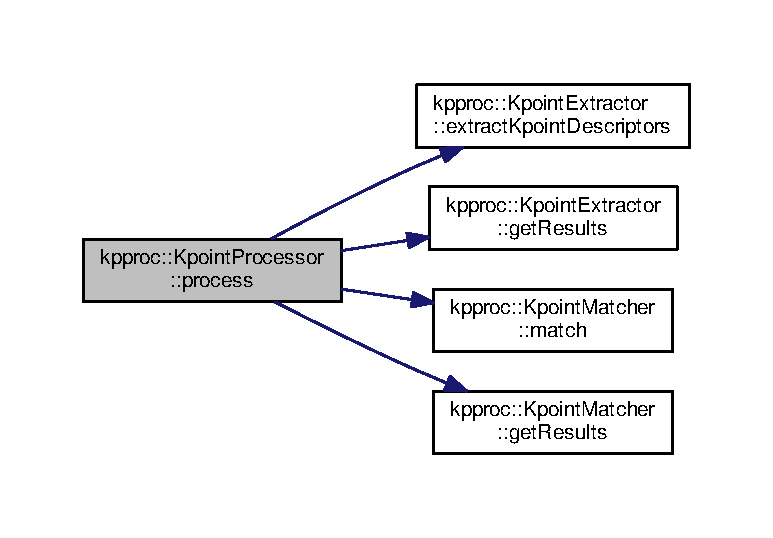
\includegraphics[width=350pt]{classkpproc_1_1KpointProcessor_a35bdf2239f6742875bbc64338488075a_cgraph}
\end{center}
\end{figure}
Here is the caller graph for this function\+:\nopagebreak
\begin{figure}[H]
\begin{center}
\leavevmode
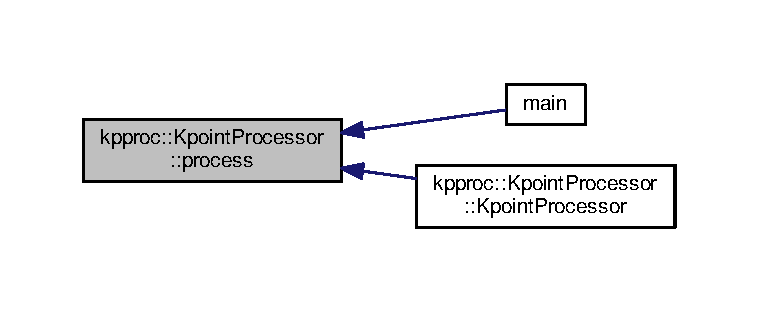
\includegraphics[width=350pt]{classkpproc_1_1KpointProcessor_a35bdf2239f6742875bbc64338488075a_icgraph}
\end{center}
\end{figure}


\subsection{Member Data Documentation}
\mbox{\Hypertarget{classkpproc_1_1KpointProcessor_a5ae3277154dd03cddf303d3be6bb37f7}\label{classkpproc_1_1KpointProcessor_a5ae3277154dd03cddf303d3be6bb37f7}} 
\index{kpproc\+::\+Kpoint\+Processor@{kpproc\+::\+Kpoint\+Processor}!m\+\_\+extractor@{m\+\_\+extractor}}
\index{m\+\_\+extractor@{m\+\_\+extractor}!kpproc\+::\+Kpoint\+Processor@{kpproc\+::\+Kpoint\+Processor}}
\subsubsection{\texorpdfstring{m\+\_\+extractor}{m\_extractor}}
{\footnotesize\ttfamily \hyperlink{classkpproc_1_1KpointExtractor}{Kpoint\+Extractor} kpproc\+::\+Kpoint\+Processor\+::m\+\_\+extractor}

\mbox{\Hypertarget{classkpproc_1_1KpointProcessor_a7faab52da545a233fab6ec061338393e}\label{classkpproc_1_1KpointProcessor_a7faab52da545a233fab6ec061338393e}} 
\index{kpproc\+::\+Kpoint\+Processor@{kpproc\+::\+Kpoint\+Processor}!m\+\_\+frame\+Buffer@{m\+\_\+frame\+Buffer}}
\index{m\+\_\+frame\+Buffer@{m\+\_\+frame\+Buffer}!kpproc\+::\+Kpoint\+Processor@{kpproc\+::\+Kpoint\+Processor}}
\subsubsection{\texorpdfstring{m\+\_\+frame\+Buffer}{m\_frameBuffer}}
{\footnotesize\ttfamily boost\+::circular\+\_\+buffer$<$\hyperlink{classFrame}{Frame}$>$\& kpproc\+::\+Kpoint\+Processor\+::m\+\_\+frame\+Buffer}

\mbox{\Hypertarget{classkpproc_1_1KpointProcessor_a188352f2093e636cbb06114b4ac7288a}\label{classkpproc_1_1KpointProcessor_a188352f2093e636cbb06114b4ac7288a}} 
\index{kpproc\+::\+Kpoint\+Processor@{kpproc\+::\+Kpoint\+Processor}!m\+\_\+matcher@{m\+\_\+matcher}}
\index{m\+\_\+matcher@{m\+\_\+matcher}!kpproc\+::\+Kpoint\+Processor@{kpproc\+::\+Kpoint\+Processor}}
\subsubsection{\texorpdfstring{m\+\_\+matcher}{m\_matcher}}
{\footnotesize\ttfamily \hyperlink{classkpproc_1_1KpointMatcher}{Kpoint\+Matcher} kpproc\+::\+Kpoint\+Processor\+::m\+\_\+matcher}

\mbox{\Hypertarget{classkpproc_1_1KpointProcessor_ac521fd8cfc2400004e729fc504209232}\label{classkpproc_1_1KpointProcessor_ac521fd8cfc2400004e729fc504209232}} 
\index{kpproc\+::\+Kpoint\+Processor@{kpproc\+::\+Kpoint\+Processor}!m\+\_\+visu\+Enable@{m\+\_\+visu\+Enable}}
\index{m\+\_\+visu\+Enable@{m\+\_\+visu\+Enable}!kpproc\+::\+Kpoint\+Processor@{kpproc\+::\+Kpoint\+Processor}}
\subsubsection{\texorpdfstring{m\+\_\+visu\+Enable}{m\_visuEnable}}
{\footnotesize\ttfamily bool kpproc\+::\+Kpoint\+Processor\+::m\+\_\+visu\+Enable\hspace{0.3cm}{\ttfamily [private]}}



The documentation for this class was generated from the following files\+:\begin{DoxyCompactItemize}
\item 
src/pose/\hyperlink{KpointProcessor_8hpp}{Kpoint\+Processor.\+hpp}\item 
src/pose/\hyperlink{KpointProcessor_8cpp}{Kpoint\+Processor.\+cpp}\end{DoxyCompactItemize}

\chapter{File Documentation}
\hypertarget{CMakeCCompilerId_8c}{}\section{build/\+C\+Make\+Files/3.5.1/\+Compiler\+Id\+C/\+C\+Make\+C\+Compiler\+Id.c File Reference}
\label{CMakeCCompilerId_8c}\index{build/\+C\+Make\+Files/3.\+5.\+1/\+Compiler\+Id\+C/\+C\+Make\+C\+Compiler\+Id.\+c@{build/\+C\+Make\+Files/3.\+5.\+1/\+Compiler\+Id\+C/\+C\+Make\+C\+Compiler\+Id.\+c}}
\subsection*{Macros}
\begin{DoxyCompactItemize}
\item 
\#define \hyperlink{CMakeCCompilerId_8c_a81dee0709ded976b2e0319239f72d174}{C\+O\+M\+P\+I\+L\+E\+R\+\_\+\+ID}~\char`\"{}\char`\"{}
\item 
\#define \hyperlink{CMakeCCompilerId_8c_a2ae9b72bb13abaabfcf2ee0ba7d3fa1d}{S\+T\+R\+I\+N\+G\+I\+F\+Y\+\_\+\+H\+E\+L\+P\+ER}(X)~\#X
\item 
\#define \hyperlink{CMakeCCompilerId_8c_a43e1cad902b6477bec893cb6430bd6c8}{S\+T\+R\+I\+N\+G\+I\+FY}(X)~\hyperlink{CMakeCXXCompilerId_8cpp_a2ae9b72bb13abaabfcf2ee0ba7d3fa1d}{S\+T\+R\+I\+N\+G\+I\+F\+Y\+\_\+\+H\+E\+L\+P\+ER}(X)
\item 
\#define \hyperlink{CMakeCCompilerId_8c_adbc5372f40838899018fadbc89bd588b}{P\+L\+A\+T\+F\+O\+R\+M\+\_\+\+ID}~\char`\"{}\char`\"{}
\item 
\#define \hyperlink{CMakeCCompilerId_8c_aba35d0d200deaeb06aee95ca297acb28}{A\+R\+C\+H\+I\+T\+E\+C\+T\+U\+R\+E\+\_\+\+ID}~\char`\"{}\char`\"{}
\item 
\#define \hyperlink{CMakeCCompilerId_8c_ad1280362da42492bbc11aa78cbf776ad}{D\+EC}(n)
\item 
\#define \hyperlink{CMakeCCompilerId_8c_a46d5d95daa1bef867bd0179594310ed5}{H\+EX}(n)
\end{DoxyCompactItemize}
\subsection*{Functions}
\begin{DoxyCompactItemize}
\item 
int \hyperlink{CMakeCCompilerId_8c_a0ddf1224851353fc92bfbff6f499fa97}{main} (int argc, char $\ast$argv\mbox{[}$\,$\mbox{]})
\end{DoxyCompactItemize}
\subsection*{Variables}
\begin{DoxyCompactItemize}
\item 
char const $\ast$ \hyperlink{CMakeCCompilerId_8c_a4b0efeb7a5d59313986b3a0390f050f6}{info\+\_\+compiler} = \char`\"{}I\+N\+FO\char`\"{} \char`\"{}\+:\char`\"{} \char`\"{}compiler\mbox{[}\char`\"{} C\+O\+M\+P\+I\+L\+E\+R\+\_\+\+ID \char`\"{}\mbox{]}\char`\"{}
\item 
char const $\ast$ \hyperlink{CMakeCCompilerId_8c_a2321403dee54ee23f0c2fa849c60f7d4}{info\+\_\+platform} = \char`\"{}I\+N\+FO\char`\"{} \char`\"{}\+:\char`\"{} \char`\"{}platform\mbox{[}\char`\"{} P\+L\+A\+T\+F\+O\+R\+M\+\_\+\+ID \char`\"{}\mbox{]}\char`\"{}
\item 
char const $\ast$ \hyperlink{CMakeCCompilerId_8c_a59647e99d304ed33b15cb284c27ed391}{info\+\_\+arch} = \char`\"{}I\+N\+FO\char`\"{} \char`\"{}\+:\char`\"{} \char`\"{}arch\mbox{[}\char`\"{} A\+R\+C\+H\+I\+T\+E\+C\+T\+U\+R\+E\+\_\+\+ID \char`\"{}\mbox{]}\char`\"{}
\item 
const char $\ast$ \hyperlink{CMakeCCompilerId_8c_a1ce162bad2fe6966ac8b33cc19e120b8}{info\+\_\+language\+\_\+dialect\+\_\+default}
\end{DoxyCompactItemize}


\subsection{Macro Definition Documentation}
\index{C\+Make\+C\+Compiler\+Id.\+c@{C\+Make\+C\+Compiler\+Id.\+c}!A\+R\+C\+H\+I\+T\+E\+C\+T\+U\+R\+E\+\_\+\+ID@{A\+R\+C\+H\+I\+T\+E\+C\+T\+U\+R\+E\+\_\+\+ID}}
\index{A\+R\+C\+H\+I\+T\+E\+C\+T\+U\+R\+E\+\_\+\+ID@{A\+R\+C\+H\+I\+T\+E\+C\+T\+U\+R\+E\+\_\+\+ID}!C\+Make\+C\+Compiler\+Id.\+c@{C\+Make\+C\+Compiler\+Id.\+c}}
\subsubsection[{\texorpdfstring{A\+R\+C\+H\+I\+T\+E\+C\+T\+U\+R\+E\+\_\+\+ID}{ARCHITECTURE_ID}}]{\setlength{\rightskip}{0pt plus 5cm}\#define A\+R\+C\+H\+I\+T\+E\+C\+T\+U\+R\+E\+\_\+\+ID~\char`\"{}\char`\"{}}\hypertarget{CMakeCCompilerId_8c_aba35d0d200deaeb06aee95ca297acb28}{}\label{CMakeCCompilerId_8c_aba35d0d200deaeb06aee95ca297acb28}
\index{C\+Make\+C\+Compiler\+Id.\+c@{C\+Make\+C\+Compiler\+Id.\+c}!C\+O\+M\+P\+I\+L\+E\+R\+\_\+\+ID@{C\+O\+M\+P\+I\+L\+E\+R\+\_\+\+ID}}
\index{C\+O\+M\+P\+I\+L\+E\+R\+\_\+\+ID@{C\+O\+M\+P\+I\+L\+E\+R\+\_\+\+ID}!C\+Make\+C\+Compiler\+Id.\+c@{C\+Make\+C\+Compiler\+Id.\+c}}
\subsubsection[{\texorpdfstring{C\+O\+M\+P\+I\+L\+E\+R\+\_\+\+ID}{COMPILER_ID}}]{\setlength{\rightskip}{0pt plus 5cm}\#define C\+O\+M\+P\+I\+L\+E\+R\+\_\+\+ID~\char`\"{}\char`\"{}}\hypertarget{CMakeCCompilerId_8c_a81dee0709ded976b2e0319239f72d174}{}\label{CMakeCCompilerId_8c_a81dee0709ded976b2e0319239f72d174}
\index{C\+Make\+C\+Compiler\+Id.\+c@{C\+Make\+C\+Compiler\+Id.\+c}!D\+EC@{D\+EC}}
\index{D\+EC@{D\+EC}!C\+Make\+C\+Compiler\+Id.\+c@{C\+Make\+C\+Compiler\+Id.\+c}}
\subsubsection[{\texorpdfstring{D\+EC}{DEC}}]{\setlength{\rightskip}{0pt plus 5cm}\#define D\+EC(
\begin{DoxyParamCaption}
\item[{}]{n}
\end{DoxyParamCaption}
)}\hypertarget{CMakeCCompilerId_8c_ad1280362da42492bbc11aa78cbf776ad}{}\label{CMakeCCompilerId_8c_ad1280362da42492bbc11aa78cbf776ad}
{\bfseries Value\+:}
\begin{DoxyCode}
(\textcolor{charliteral}{'0'} + (((n) / 10000000)%10)), \(\backslash\)
  (\textcolor{charliteral}{'0'} + (((n) / 1000000)%10)),  \(\backslash\)
  (\textcolor{charliteral}{'0'} + (((n) / 100000)%10)),   \(\backslash\)
  (\textcolor{charliteral}{'0'} + (((n) / 10000)%10)),    \(\backslash\)
  (\textcolor{charliteral}{'0'} + (((n) / 1000)%10)),     \(\backslash\)
  (\textcolor{charliteral}{'0'} + (((n) / 100)%10)),      \(\backslash\)
  (\textcolor{charliteral}{'0'} + (((n) / 10)%10)),       \(\backslash\)
  (\textcolor{charliteral}{'0'} +  ((n) % 10))
\end{DoxyCode}
\index{C\+Make\+C\+Compiler\+Id.\+c@{C\+Make\+C\+Compiler\+Id.\+c}!H\+EX@{H\+EX}}
\index{H\+EX@{H\+EX}!C\+Make\+C\+Compiler\+Id.\+c@{C\+Make\+C\+Compiler\+Id.\+c}}
\subsubsection[{\texorpdfstring{H\+EX}{HEX}}]{\setlength{\rightskip}{0pt plus 5cm}\#define H\+EX(
\begin{DoxyParamCaption}
\item[{}]{n}
\end{DoxyParamCaption}
)}\hypertarget{CMakeCCompilerId_8c_a46d5d95daa1bef867bd0179594310ed5}{}\label{CMakeCCompilerId_8c_a46d5d95daa1bef867bd0179594310ed5}
{\bfseries Value\+:}
\begin{DoxyCode}
(\textcolor{charliteral}{'0'} + ((n)>>28 & 0xF)), \(\backslash\)
  (\textcolor{charliteral}{'0'} + ((n)>>24 & 0xF)), \(\backslash\)
  (\textcolor{charliteral}{'0'} + ((n)>>20 & 0xF)), \(\backslash\)
  (\textcolor{charliteral}{'0'} + ((n)>>16 & 0xF)), \(\backslash\)
  (\textcolor{charliteral}{'0'} + ((n)>>12 & 0xF)), \(\backslash\)
  (\textcolor{charliteral}{'0'} + ((n)>>8  & 0xF)), \(\backslash\)
  (\textcolor{charliteral}{'0'} + ((n)>>4  & 0xF)), \(\backslash\)
  (\textcolor{charliteral}{'0'} + ((n)     & 0xF))
\end{DoxyCode}
\index{C\+Make\+C\+Compiler\+Id.\+c@{C\+Make\+C\+Compiler\+Id.\+c}!P\+L\+A\+T\+F\+O\+R\+M\+\_\+\+ID@{P\+L\+A\+T\+F\+O\+R\+M\+\_\+\+ID}}
\index{P\+L\+A\+T\+F\+O\+R\+M\+\_\+\+ID@{P\+L\+A\+T\+F\+O\+R\+M\+\_\+\+ID}!C\+Make\+C\+Compiler\+Id.\+c@{C\+Make\+C\+Compiler\+Id.\+c}}
\subsubsection[{\texorpdfstring{P\+L\+A\+T\+F\+O\+R\+M\+\_\+\+ID}{PLATFORM_ID}}]{\setlength{\rightskip}{0pt plus 5cm}\#define P\+L\+A\+T\+F\+O\+R\+M\+\_\+\+ID~\char`\"{}\char`\"{}}\hypertarget{CMakeCCompilerId_8c_adbc5372f40838899018fadbc89bd588b}{}\label{CMakeCCompilerId_8c_adbc5372f40838899018fadbc89bd588b}
\index{C\+Make\+C\+Compiler\+Id.\+c@{C\+Make\+C\+Compiler\+Id.\+c}!S\+T\+R\+I\+N\+G\+I\+FY@{S\+T\+R\+I\+N\+G\+I\+FY}}
\index{S\+T\+R\+I\+N\+G\+I\+FY@{S\+T\+R\+I\+N\+G\+I\+FY}!C\+Make\+C\+Compiler\+Id.\+c@{C\+Make\+C\+Compiler\+Id.\+c}}
\subsubsection[{\texorpdfstring{S\+T\+R\+I\+N\+G\+I\+FY}{STRINGIFY}}]{\setlength{\rightskip}{0pt plus 5cm}\#define S\+T\+R\+I\+N\+G\+I\+FY(
\begin{DoxyParamCaption}
\item[{}]{X}
\end{DoxyParamCaption}
)~{\bf S\+T\+R\+I\+N\+G\+I\+F\+Y\+\_\+\+H\+E\+L\+P\+ER}(X)}\hypertarget{CMakeCCompilerId_8c_a43e1cad902b6477bec893cb6430bd6c8}{}\label{CMakeCCompilerId_8c_a43e1cad902b6477bec893cb6430bd6c8}
\index{C\+Make\+C\+Compiler\+Id.\+c@{C\+Make\+C\+Compiler\+Id.\+c}!S\+T\+R\+I\+N\+G\+I\+F\+Y\+\_\+\+H\+E\+L\+P\+ER@{S\+T\+R\+I\+N\+G\+I\+F\+Y\+\_\+\+H\+E\+L\+P\+ER}}
\index{S\+T\+R\+I\+N\+G\+I\+F\+Y\+\_\+\+H\+E\+L\+P\+ER@{S\+T\+R\+I\+N\+G\+I\+F\+Y\+\_\+\+H\+E\+L\+P\+ER}!C\+Make\+C\+Compiler\+Id.\+c@{C\+Make\+C\+Compiler\+Id.\+c}}
\subsubsection[{\texorpdfstring{S\+T\+R\+I\+N\+G\+I\+F\+Y\+\_\+\+H\+E\+L\+P\+ER}{STRINGIFY_HELPER}}]{\setlength{\rightskip}{0pt plus 5cm}\#define S\+T\+R\+I\+N\+G\+I\+F\+Y\+\_\+\+H\+E\+L\+P\+ER(
\begin{DoxyParamCaption}
\item[{}]{X}
\end{DoxyParamCaption}
)~\#X}\hypertarget{CMakeCCompilerId_8c_a2ae9b72bb13abaabfcf2ee0ba7d3fa1d}{}\label{CMakeCCompilerId_8c_a2ae9b72bb13abaabfcf2ee0ba7d3fa1d}


\subsection{Function Documentation}
\index{C\+Make\+C\+Compiler\+Id.\+c@{C\+Make\+C\+Compiler\+Id.\+c}!main@{main}}
\index{main@{main}!C\+Make\+C\+Compiler\+Id.\+c@{C\+Make\+C\+Compiler\+Id.\+c}}
\subsubsection[{\texorpdfstring{main(int argc, char $\ast$argv[])}{main(int argc, char *argv[])}}]{\setlength{\rightskip}{0pt plus 5cm}int main (
\begin{DoxyParamCaption}
\item[{int}]{argc, }
\item[{char $\ast$}]{argv\mbox{[}$\,$\mbox{]}}
\end{DoxyParamCaption}
)}\hypertarget{CMakeCCompilerId_8c_a0ddf1224851353fc92bfbff6f499fa97}{}\label{CMakeCCompilerId_8c_a0ddf1224851353fc92bfbff6f499fa97}


\subsection{Variable Documentation}
\index{C\+Make\+C\+Compiler\+Id.\+c@{C\+Make\+C\+Compiler\+Id.\+c}!info\+\_\+arch@{info\+\_\+arch}}
\index{info\+\_\+arch@{info\+\_\+arch}!C\+Make\+C\+Compiler\+Id.\+c@{C\+Make\+C\+Compiler\+Id.\+c}}
\subsubsection[{\texorpdfstring{info\+\_\+arch}{info_arch}}]{\setlength{\rightskip}{0pt plus 5cm}char const$\ast$ info\+\_\+arch = \char`\"{}I\+N\+FO\char`\"{} \char`\"{}\+:\char`\"{} \char`\"{}arch\mbox{[}\char`\"{} A\+R\+C\+H\+I\+T\+E\+C\+T\+U\+R\+E\+\_\+\+ID \char`\"{}\mbox{]}\char`\"{}}\hypertarget{CMakeCCompilerId_8c_a59647e99d304ed33b15cb284c27ed391}{}\label{CMakeCCompilerId_8c_a59647e99d304ed33b15cb284c27ed391}
\index{C\+Make\+C\+Compiler\+Id.\+c@{C\+Make\+C\+Compiler\+Id.\+c}!info\+\_\+compiler@{info\+\_\+compiler}}
\index{info\+\_\+compiler@{info\+\_\+compiler}!C\+Make\+C\+Compiler\+Id.\+c@{C\+Make\+C\+Compiler\+Id.\+c}}
\subsubsection[{\texorpdfstring{info\+\_\+compiler}{info_compiler}}]{\setlength{\rightskip}{0pt plus 5cm}char const$\ast$ info\+\_\+compiler = \char`\"{}I\+N\+FO\char`\"{} \char`\"{}\+:\char`\"{} \char`\"{}compiler\mbox{[}\char`\"{} C\+O\+M\+P\+I\+L\+E\+R\+\_\+\+ID \char`\"{}\mbox{]}\char`\"{}}\hypertarget{CMakeCCompilerId_8c_a4b0efeb7a5d59313986b3a0390f050f6}{}\label{CMakeCCompilerId_8c_a4b0efeb7a5d59313986b3a0390f050f6}
\index{C\+Make\+C\+Compiler\+Id.\+c@{C\+Make\+C\+Compiler\+Id.\+c}!info\+\_\+language\+\_\+dialect\+\_\+default@{info\+\_\+language\+\_\+dialect\+\_\+default}}
\index{info\+\_\+language\+\_\+dialect\+\_\+default@{info\+\_\+language\+\_\+dialect\+\_\+default}!C\+Make\+C\+Compiler\+Id.\+c@{C\+Make\+C\+Compiler\+Id.\+c}}
\subsubsection[{\texorpdfstring{info\+\_\+language\+\_\+dialect\+\_\+default}{info_language_dialect_default}}]{\setlength{\rightskip}{0pt plus 5cm}const char$\ast$ info\+\_\+language\+\_\+dialect\+\_\+default}\hypertarget{CMakeCCompilerId_8c_a1ce162bad2fe6966ac8b33cc19e120b8}{}\label{CMakeCCompilerId_8c_a1ce162bad2fe6966ac8b33cc19e120b8}
{\bfseries Initial value\+:}
\begin{DoxyCode}
= \textcolor{stringliteral}{"INFO"} \textcolor{stringliteral}{":"} \textcolor{stringliteral}{"dialect\_default["}

  \textcolor{stringliteral}{"90"}






\textcolor{stringliteral}{"]"}
\end{DoxyCode}
\index{C\+Make\+C\+Compiler\+Id.\+c@{C\+Make\+C\+Compiler\+Id.\+c}!info\+\_\+platform@{info\+\_\+platform}}
\index{info\+\_\+platform@{info\+\_\+platform}!C\+Make\+C\+Compiler\+Id.\+c@{C\+Make\+C\+Compiler\+Id.\+c}}
\subsubsection[{\texorpdfstring{info\+\_\+platform}{info_platform}}]{\setlength{\rightskip}{0pt plus 5cm}char const$\ast$ info\+\_\+platform = \char`\"{}I\+N\+FO\char`\"{} \char`\"{}\+:\char`\"{} \char`\"{}platform\mbox{[}\char`\"{} P\+L\+A\+T\+F\+O\+R\+M\+\_\+\+ID \char`\"{}\mbox{]}\char`\"{}}\hypertarget{CMakeCCompilerId_8c_a2321403dee54ee23f0c2fa849c60f7d4}{}\label{CMakeCCompilerId_8c_a2321403dee54ee23f0c2fa849c60f7d4}

\hypertarget{CMakeCXXCompilerId_8cpp}{}\section{build/\+C\+Make\+Files/3.10.2/\+Compiler\+Id\+C\+X\+X/\+C\+Make\+C\+X\+X\+Compiler\+Id.cpp File Reference}
\label{CMakeCXXCompilerId_8cpp}\index{build/\+C\+Make\+Files/3.\+10.\+2/\+Compiler\+Id\+C\+X\+X/\+C\+Make\+C\+X\+X\+Compiler\+Id.\+cpp@{build/\+C\+Make\+Files/3.\+10.\+2/\+Compiler\+Id\+C\+X\+X/\+C\+Make\+C\+X\+X\+Compiler\+Id.\+cpp}}
\subsection*{Macros}
\begin{DoxyCompactItemize}
\item 
\#define \hyperlink{CMakeCXXCompilerId_8cpp_a81dee0709ded976b2e0319239f72d174}{C\+O\+M\+P\+I\+L\+E\+R\+\_\+\+ID}~\char`\"{}\char`\"{}
\item 
\#define \hyperlink{CMakeCXXCompilerId_8cpp_a2ae9b72bb13abaabfcf2ee0ba7d3fa1d}{S\+T\+R\+I\+N\+G\+I\+F\+Y\+\_\+\+H\+E\+L\+P\+ER}(X)~\#X
\item 
\#define \hyperlink{CMakeCXXCompilerId_8cpp_a43e1cad902b6477bec893cb6430bd6c8}{S\+T\+R\+I\+N\+G\+I\+FY}(X)~\hyperlink{CMakeCXXCompilerId_8cpp_a2ae9b72bb13abaabfcf2ee0ba7d3fa1d}{S\+T\+R\+I\+N\+G\+I\+F\+Y\+\_\+\+H\+E\+L\+P\+ER}(X)
\item 
\#define \hyperlink{CMakeCXXCompilerId_8cpp_adbc5372f40838899018fadbc89bd588b}{P\+L\+A\+T\+F\+O\+R\+M\+\_\+\+ID}
\item 
\#define \hyperlink{CMakeCXXCompilerId_8cpp_aba35d0d200deaeb06aee95ca297acb28}{A\+R\+C\+H\+I\+T\+E\+C\+T\+U\+R\+E\+\_\+\+ID}
\item 
\#define \hyperlink{CMakeCXXCompilerId_8cpp_ad1280362da42492bbc11aa78cbf776ad}{D\+EC}(n)
\item 
\#define \hyperlink{CMakeCXXCompilerId_8cpp_a46d5d95daa1bef867bd0179594310ed5}{H\+EX}(n)
\item 
\#define \hyperlink{CMakeCXXCompilerId_8cpp_a34cc889e576a1ae6c84ae9e0a851ba21}{C\+X\+X\+\_\+\+S\+TD}~\+\_\+\+\_\+cplusplus
\end{DoxyCompactItemize}
\subsection*{Functions}
\begin{DoxyCompactItemize}
\item 
int \hyperlink{CMakeCXXCompilerId_8cpp_a0ddf1224851353fc92bfbff6f499fa97}{main} (int argc, char $\ast$argv\mbox{[}$\,$\mbox{]})
\end{DoxyCompactItemize}
\subsection*{Variables}
\begin{DoxyCompactItemize}
\item 
char const  $\ast$ \hyperlink{CMakeCXXCompilerId_8cpp_a4b0efeb7a5d59313986b3a0390f050f6}{info\+\_\+compiler} = \char`\"{}I\+N\+FO\char`\"{} \char`\"{}\+:\char`\"{} \char`\"{}compiler\mbox{[}\char`\"{} C\+O\+M\+P\+I\+L\+E\+R\+\_\+\+ID \char`\"{}\mbox{]}\char`\"{}
\item 
char const  $\ast$ \hyperlink{CMakeCXXCompilerId_8cpp_a2321403dee54ee23f0c2fa849c60f7d4}{info\+\_\+platform} = \char`\"{}I\+N\+FO\char`\"{} \char`\"{}\+:\char`\"{} \char`\"{}platform\mbox{[}\char`\"{} P\+L\+A\+T\+F\+O\+R\+M\+\_\+\+ID \char`\"{}\mbox{]}\char`\"{}
\item 
char const  $\ast$ \hyperlink{CMakeCXXCompilerId_8cpp_a59647e99d304ed33b15cb284c27ed391}{info\+\_\+arch} = \char`\"{}I\+N\+FO\char`\"{} \char`\"{}\+:\char`\"{} \char`\"{}arch\mbox{[}\char`\"{} A\+R\+C\+H\+I\+T\+E\+C\+T\+U\+R\+E\+\_\+\+ID \char`\"{}\mbox{]}\char`\"{}
\item 
const char $\ast$ \hyperlink{CMakeCXXCompilerId_8cpp_a1ce162bad2fe6966ac8b33cc19e120b8}{info\+\_\+language\+\_\+dialect\+\_\+default}
\end{DoxyCompactItemize}


\subsection{Macro Definition Documentation}
\mbox{\Hypertarget{CMakeCXXCompilerId_8cpp_aba35d0d200deaeb06aee95ca297acb28}\label{CMakeCXXCompilerId_8cpp_aba35d0d200deaeb06aee95ca297acb28}} 
\index{C\+Make\+C\+X\+X\+Compiler\+Id.\+cpp@{C\+Make\+C\+X\+X\+Compiler\+Id.\+cpp}!A\+R\+C\+H\+I\+T\+E\+C\+T\+U\+R\+E\+\_\+\+ID@{A\+R\+C\+H\+I\+T\+E\+C\+T\+U\+R\+E\+\_\+\+ID}}
\index{A\+R\+C\+H\+I\+T\+E\+C\+T\+U\+R\+E\+\_\+\+ID@{A\+R\+C\+H\+I\+T\+E\+C\+T\+U\+R\+E\+\_\+\+ID}!C\+Make\+C\+X\+X\+Compiler\+Id.\+cpp@{C\+Make\+C\+X\+X\+Compiler\+Id.\+cpp}}
\subsubsection{\texorpdfstring{A\+R\+C\+H\+I\+T\+E\+C\+T\+U\+R\+E\+\_\+\+ID}{ARCHITECTURE\_ID}}
{\footnotesize\ttfamily \#define A\+R\+C\+H\+I\+T\+E\+C\+T\+U\+R\+E\+\_\+\+ID}

\mbox{\Hypertarget{CMakeCXXCompilerId_8cpp_a81dee0709ded976b2e0319239f72d174}\label{CMakeCXXCompilerId_8cpp_a81dee0709ded976b2e0319239f72d174}} 
\index{C\+Make\+C\+X\+X\+Compiler\+Id.\+cpp@{C\+Make\+C\+X\+X\+Compiler\+Id.\+cpp}!C\+O\+M\+P\+I\+L\+E\+R\+\_\+\+ID@{C\+O\+M\+P\+I\+L\+E\+R\+\_\+\+ID}}
\index{C\+O\+M\+P\+I\+L\+E\+R\+\_\+\+ID@{C\+O\+M\+P\+I\+L\+E\+R\+\_\+\+ID}!C\+Make\+C\+X\+X\+Compiler\+Id.\+cpp@{C\+Make\+C\+X\+X\+Compiler\+Id.\+cpp}}
\subsubsection{\texorpdfstring{C\+O\+M\+P\+I\+L\+E\+R\+\_\+\+ID}{COMPILER\_ID}}
{\footnotesize\ttfamily \#define C\+O\+M\+P\+I\+L\+E\+R\+\_\+\+ID~\char`\"{}\char`\"{}}

\mbox{\Hypertarget{CMakeCXXCompilerId_8cpp_a34cc889e576a1ae6c84ae9e0a851ba21}\label{CMakeCXXCompilerId_8cpp_a34cc889e576a1ae6c84ae9e0a851ba21}} 
\index{C\+Make\+C\+X\+X\+Compiler\+Id.\+cpp@{C\+Make\+C\+X\+X\+Compiler\+Id.\+cpp}!C\+X\+X\+\_\+\+S\+TD@{C\+X\+X\+\_\+\+S\+TD}}
\index{C\+X\+X\+\_\+\+S\+TD@{C\+X\+X\+\_\+\+S\+TD}!C\+Make\+C\+X\+X\+Compiler\+Id.\+cpp@{C\+Make\+C\+X\+X\+Compiler\+Id.\+cpp}}
\subsubsection{\texorpdfstring{C\+X\+X\+\_\+\+S\+TD}{CXX\_STD}}
{\footnotesize\ttfamily \#define C\+X\+X\+\_\+\+S\+TD~\+\_\+\+\_\+cplusplus}

\mbox{\Hypertarget{CMakeCXXCompilerId_8cpp_ad1280362da42492bbc11aa78cbf776ad}\label{CMakeCXXCompilerId_8cpp_ad1280362da42492bbc11aa78cbf776ad}} 
\index{C\+Make\+C\+X\+X\+Compiler\+Id.\+cpp@{C\+Make\+C\+X\+X\+Compiler\+Id.\+cpp}!D\+EC@{D\+EC}}
\index{D\+EC@{D\+EC}!C\+Make\+C\+X\+X\+Compiler\+Id.\+cpp@{C\+Make\+C\+X\+X\+Compiler\+Id.\+cpp}}
\subsubsection{\texorpdfstring{D\+EC}{DEC}}
{\footnotesize\ttfamily \#define D\+EC(\begin{DoxyParamCaption}\item[{}]{n }\end{DoxyParamCaption})}

{\bfseries Value\+:}
\begin{DoxyCode}
(\textcolor{charliteral}{'0'} + (((n) / 10000000)%10)), \(\backslash\)
  (\textcolor{charliteral}{'0'} + (((n) / 1000000)%10)),  \(\backslash\)
  (\textcolor{charliteral}{'0'} + (((n) / 100000)%10)),   \(\backslash\)
  (\textcolor{charliteral}{'0'} + (((n) / 10000)%10)),    \(\backslash\)
  (\textcolor{charliteral}{'0'} + (((n) / 1000)%10)),     \(\backslash\)
  (\textcolor{charliteral}{'0'} + (((n) / 100)%10)),      \(\backslash\)
  (\textcolor{charliteral}{'0'} + (((n) / 10)%10)),       \(\backslash\)
  (\textcolor{charliteral}{'0'} +  ((n) % 10))
\end{DoxyCode}
\mbox{\Hypertarget{CMakeCXXCompilerId_8cpp_a46d5d95daa1bef867bd0179594310ed5}\label{CMakeCXXCompilerId_8cpp_a46d5d95daa1bef867bd0179594310ed5}} 
\index{C\+Make\+C\+X\+X\+Compiler\+Id.\+cpp@{C\+Make\+C\+X\+X\+Compiler\+Id.\+cpp}!H\+EX@{H\+EX}}
\index{H\+EX@{H\+EX}!C\+Make\+C\+X\+X\+Compiler\+Id.\+cpp@{C\+Make\+C\+X\+X\+Compiler\+Id.\+cpp}}
\subsubsection{\texorpdfstring{H\+EX}{HEX}}
{\footnotesize\ttfamily \#define H\+EX(\begin{DoxyParamCaption}\item[{}]{n }\end{DoxyParamCaption})}

{\bfseries Value\+:}
\begin{DoxyCode}
(\textcolor{charliteral}{'0'} + ((n)>>28 & 0xF)), \(\backslash\)
  (\textcolor{charliteral}{'0'} + ((n)>>24 & 0xF)), \(\backslash\)
  (\textcolor{charliteral}{'0'} + ((n)>>20 & 0xF)), \(\backslash\)
  (\textcolor{charliteral}{'0'} + ((n)>>16 & 0xF)), \(\backslash\)
  (\textcolor{charliteral}{'0'} + ((n)>>12 & 0xF)), \(\backslash\)
  (\textcolor{charliteral}{'0'} + ((n)>>8  & 0xF)), \(\backslash\)
  (\textcolor{charliteral}{'0'} + ((n)>>4  & 0xF)), \(\backslash\)
  (\textcolor{charliteral}{'0'} + ((n)     & 0xF))
\end{DoxyCode}
\mbox{\Hypertarget{CMakeCXXCompilerId_8cpp_adbc5372f40838899018fadbc89bd588b}\label{CMakeCXXCompilerId_8cpp_adbc5372f40838899018fadbc89bd588b}} 
\index{C\+Make\+C\+X\+X\+Compiler\+Id.\+cpp@{C\+Make\+C\+X\+X\+Compiler\+Id.\+cpp}!P\+L\+A\+T\+F\+O\+R\+M\+\_\+\+ID@{P\+L\+A\+T\+F\+O\+R\+M\+\_\+\+ID}}
\index{P\+L\+A\+T\+F\+O\+R\+M\+\_\+\+ID@{P\+L\+A\+T\+F\+O\+R\+M\+\_\+\+ID}!C\+Make\+C\+X\+X\+Compiler\+Id.\+cpp@{C\+Make\+C\+X\+X\+Compiler\+Id.\+cpp}}
\subsubsection{\texorpdfstring{P\+L\+A\+T\+F\+O\+R\+M\+\_\+\+ID}{PLATFORM\_ID}}
{\footnotesize\ttfamily \#define P\+L\+A\+T\+F\+O\+R\+M\+\_\+\+ID}

\mbox{\Hypertarget{CMakeCXXCompilerId_8cpp_a43e1cad902b6477bec893cb6430bd6c8}\label{CMakeCXXCompilerId_8cpp_a43e1cad902b6477bec893cb6430bd6c8}} 
\index{C\+Make\+C\+X\+X\+Compiler\+Id.\+cpp@{C\+Make\+C\+X\+X\+Compiler\+Id.\+cpp}!S\+T\+R\+I\+N\+G\+I\+FY@{S\+T\+R\+I\+N\+G\+I\+FY}}
\index{S\+T\+R\+I\+N\+G\+I\+FY@{S\+T\+R\+I\+N\+G\+I\+FY}!C\+Make\+C\+X\+X\+Compiler\+Id.\+cpp@{C\+Make\+C\+X\+X\+Compiler\+Id.\+cpp}}
\subsubsection{\texorpdfstring{S\+T\+R\+I\+N\+G\+I\+FY}{STRINGIFY}}
{\footnotesize\ttfamily \#define S\+T\+R\+I\+N\+G\+I\+FY(\begin{DoxyParamCaption}\item[{}]{X }\end{DoxyParamCaption})~\hyperlink{CMakeCXXCompilerId_8cpp_a2ae9b72bb13abaabfcf2ee0ba7d3fa1d}{S\+T\+R\+I\+N\+G\+I\+F\+Y\+\_\+\+H\+E\+L\+P\+ER}(X)}

\mbox{\Hypertarget{CMakeCXXCompilerId_8cpp_a2ae9b72bb13abaabfcf2ee0ba7d3fa1d}\label{CMakeCXXCompilerId_8cpp_a2ae9b72bb13abaabfcf2ee0ba7d3fa1d}} 
\index{C\+Make\+C\+X\+X\+Compiler\+Id.\+cpp@{C\+Make\+C\+X\+X\+Compiler\+Id.\+cpp}!S\+T\+R\+I\+N\+G\+I\+F\+Y\+\_\+\+H\+E\+L\+P\+ER@{S\+T\+R\+I\+N\+G\+I\+F\+Y\+\_\+\+H\+E\+L\+P\+ER}}
\index{S\+T\+R\+I\+N\+G\+I\+F\+Y\+\_\+\+H\+E\+L\+P\+ER@{S\+T\+R\+I\+N\+G\+I\+F\+Y\+\_\+\+H\+E\+L\+P\+ER}!C\+Make\+C\+X\+X\+Compiler\+Id.\+cpp@{C\+Make\+C\+X\+X\+Compiler\+Id.\+cpp}}
\subsubsection{\texorpdfstring{S\+T\+R\+I\+N\+G\+I\+F\+Y\+\_\+\+H\+E\+L\+P\+ER}{STRINGIFY\_HELPER}}
{\footnotesize\ttfamily \#define S\+T\+R\+I\+N\+G\+I\+F\+Y\+\_\+\+H\+E\+L\+P\+ER(\begin{DoxyParamCaption}\item[{}]{X }\end{DoxyParamCaption})~\#X}



\subsection{Function Documentation}
\mbox{\Hypertarget{CMakeCXXCompilerId_8cpp_a0ddf1224851353fc92bfbff6f499fa97}\label{CMakeCXXCompilerId_8cpp_a0ddf1224851353fc92bfbff6f499fa97}} 
\index{C\+Make\+C\+X\+X\+Compiler\+Id.\+cpp@{C\+Make\+C\+X\+X\+Compiler\+Id.\+cpp}!main@{main}}
\index{main@{main}!C\+Make\+C\+X\+X\+Compiler\+Id.\+cpp@{C\+Make\+C\+X\+X\+Compiler\+Id.\+cpp}}
\subsubsection{\texorpdfstring{main()}{main()}}
{\footnotesize\ttfamily int main (\begin{DoxyParamCaption}\item[{int}]{argc,  }\item[{char $\ast$}]{argv\mbox{[}$\,$\mbox{]} }\end{DoxyParamCaption})}



\subsection{Variable Documentation}
\mbox{\Hypertarget{CMakeCXXCompilerId_8cpp_a59647e99d304ed33b15cb284c27ed391}\label{CMakeCXXCompilerId_8cpp_a59647e99d304ed33b15cb284c27ed391}} 
\index{C\+Make\+C\+X\+X\+Compiler\+Id.\+cpp@{C\+Make\+C\+X\+X\+Compiler\+Id.\+cpp}!info\+\_\+arch@{info\+\_\+arch}}
\index{info\+\_\+arch@{info\+\_\+arch}!C\+Make\+C\+X\+X\+Compiler\+Id.\+cpp@{C\+Make\+C\+X\+X\+Compiler\+Id.\+cpp}}
\subsubsection{\texorpdfstring{info\+\_\+arch}{info\_arch}}
{\footnotesize\ttfamily char const$\ast$ info\+\_\+arch = \char`\"{}I\+N\+FO\char`\"{} \char`\"{}\+:\char`\"{} \char`\"{}arch\mbox{[}\char`\"{} A\+R\+C\+H\+I\+T\+E\+C\+T\+U\+R\+E\+\_\+\+ID \char`\"{}\mbox{]}\char`\"{}}

\mbox{\Hypertarget{CMakeCXXCompilerId_8cpp_a4b0efeb7a5d59313986b3a0390f050f6}\label{CMakeCXXCompilerId_8cpp_a4b0efeb7a5d59313986b3a0390f050f6}} 
\index{C\+Make\+C\+X\+X\+Compiler\+Id.\+cpp@{C\+Make\+C\+X\+X\+Compiler\+Id.\+cpp}!info\+\_\+compiler@{info\+\_\+compiler}}
\index{info\+\_\+compiler@{info\+\_\+compiler}!C\+Make\+C\+X\+X\+Compiler\+Id.\+cpp@{C\+Make\+C\+X\+X\+Compiler\+Id.\+cpp}}
\subsubsection{\texorpdfstring{info\+\_\+compiler}{info\_compiler}}
{\footnotesize\ttfamily char const$\ast$ info\+\_\+compiler = \char`\"{}I\+N\+FO\char`\"{} \char`\"{}\+:\char`\"{} \char`\"{}compiler\mbox{[}\char`\"{} C\+O\+M\+P\+I\+L\+E\+R\+\_\+\+ID \char`\"{}\mbox{]}\char`\"{}}

\mbox{\Hypertarget{CMakeCXXCompilerId_8cpp_a1ce162bad2fe6966ac8b33cc19e120b8}\label{CMakeCXXCompilerId_8cpp_a1ce162bad2fe6966ac8b33cc19e120b8}} 
\index{C\+Make\+C\+X\+X\+Compiler\+Id.\+cpp@{C\+Make\+C\+X\+X\+Compiler\+Id.\+cpp}!info\+\_\+language\+\_\+dialect\+\_\+default@{info\+\_\+language\+\_\+dialect\+\_\+default}}
\index{info\+\_\+language\+\_\+dialect\+\_\+default@{info\+\_\+language\+\_\+dialect\+\_\+default}!C\+Make\+C\+X\+X\+Compiler\+Id.\+cpp@{C\+Make\+C\+X\+X\+Compiler\+Id.\+cpp}}
\subsubsection{\texorpdfstring{info\+\_\+language\+\_\+dialect\+\_\+default}{info\_language\_dialect\_default}}
{\footnotesize\ttfamily const char$\ast$ info\+\_\+language\+\_\+dialect\+\_\+default}

{\bfseries Initial value\+:}
\begin{DoxyCode}
= \textcolor{stringliteral}{"INFO"} \textcolor{stringliteral}{":"} \textcolor{stringliteral}{"dialect\_default["}







  \textcolor{stringliteral}{"98"}

\textcolor{stringliteral}{"]"}
\end{DoxyCode}
\mbox{\Hypertarget{CMakeCXXCompilerId_8cpp_a2321403dee54ee23f0c2fa849c60f7d4}\label{CMakeCXXCompilerId_8cpp_a2321403dee54ee23f0c2fa849c60f7d4}} 
\index{C\+Make\+C\+X\+X\+Compiler\+Id.\+cpp@{C\+Make\+C\+X\+X\+Compiler\+Id.\+cpp}!info\+\_\+platform@{info\+\_\+platform}}
\index{info\+\_\+platform@{info\+\_\+platform}!C\+Make\+C\+X\+X\+Compiler\+Id.\+cpp@{C\+Make\+C\+X\+X\+Compiler\+Id.\+cpp}}
\subsubsection{\texorpdfstring{info\+\_\+platform}{info\_platform}}
{\footnotesize\ttfamily char const$\ast$ info\+\_\+platform = \char`\"{}I\+N\+FO\char`\"{} \char`\"{}\+:\char`\"{} \char`\"{}platform\mbox{[}\char`\"{} P\+L\+A\+T\+F\+O\+R\+M\+\_\+\+ID \char`\"{}\mbox{]}\char`\"{}}


\hypertarget{feature__tests_8c}{}\section{build/\+C\+Make\+Files/feature\+\_\+tests.c File Reference}
\label{feature__tests_8c}\index{build/\+C\+Make\+Files/feature\+\_\+tests.\+c@{build/\+C\+Make\+Files/feature\+\_\+tests.\+c}}
\subsection*{Functions}
\begin{DoxyCompactItemize}
\item 
int \hyperlink{feature__tests_8c_a3c04138a5bfe5d72780bb7e82a18e627}{main} (int argc, char $\ast$$\ast$argv)
\end{DoxyCompactItemize}
\subsection*{Variables}
\begin{DoxyCompactItemize}
\item 
const char \hyperlink{feature__tests_8c_a1582568e32f689337602a16bf8a5bff0}{features} \mbox{[}$\,$\mbox{]}
\end{DoxyCompactItemize}


\subsection{Function Documentation}
\index{feature\+\_\+tests.\+c@{feature\+\_\+tests.\+c}!main@{main}}
\index{main@{main}!feature\+\_\+tests.\+c@{feature\+\_\+tests.\+c}}
\subsubsection[{\texorpdfstring{main(int argc, char $\ast$$\ast$argv)}{main(int argc, char **argv)}}]{\setlength{\rightskip}{0pt plus 5cm}int main (
\begin{DoxyParamCaption}
\item[{int}]{argc, }
\item[{char $\ast$$\ast$}]{argv}
\end{DoxyParamCaption}
)}\hypertarget{feature__tests_8c_a3c04138a5bfe5d72780bb7e82a18e627}{}\label{feature__tests_8c_a3c04138a5bfe5d72780bb7e82a18e627}


\subsection{Variable Documentation}
\index{feature\+\_\+tests.\+c@{feature\+\_\+tests.\+c}!features@{features}}
\index{features@{features}!feature\+\_\+tests.\+c@{feature\+\_\+tests.\+c}}
\subsubsection[{\texorpdfstring{features}{features}}]{\setlength{\rightskip}{0pt plus 5cm}const char features\mbox{[}$\,$\mbox{]}}\hypertarget{feature__tests_8c_a1582568e32f689337602a16bf8a5bff0}{}\label{feature__tests_8c_a1582568e32f689337602a16bf8a5bff0}

\hypertarget{feature__tests_8cxx}{}\section{build/\+C\+Make\+Files/feature\+\_\+tests.cxx File Reference}
\label{feature__tests_8cxx}\index{build/\+C\+Make\+Files/feature\+\_\+tests.\+cxx@{build/\+C\+Make\+Files/feature\+\_\+tests.\+cxx}}
\subsection*{Functions}
\begin{DoxyCompactItemize}
\item 
int \hyperlink{feature__tests_8cxx_a3c04138a5bfe5d72780bb7e82a18e627}{main} (int argc, char $\ast$$\ast$argv)
\end{DoxyCompactItemize}
\subsection*{Variables}
\begin{DoxyCompactItemize}
\item 
const char \hyperlink{feature__tests_8cxx_a1582568e32f689337602a16bf8a5bff0}{features} \mbox{[}$\,$\mbox{]}
\end{DoxyCompactItemize}


\subsection{Function Documentation}
\index{feature\+\_\+tests.\+cxx@{feature\+\_\+tests.\+cxx}!main@{main}}
\index{main@{main}!feature\+\_\+tests.\+cxx@{feature\+\_\+tests.\+cxx}}
\subsubsection[{\texorpdfstring{main(int argc, char $\ast$$\ast$argv)}{main(int argc, char **argv)}}]{\setlength{\rightskip}{0pt plus 5cm}int main (
\begin{DoxyParamCaption}
\item[{int}]{argc, }
\item[{char $\ast$$\ast$}]{argv}
\end{DoxyParamCaption}
)}\hypertarget{feature__tests_8cxx_a3c04138a5bfe5d72780bb7e82a18e627}{}\label{feature__tests_8cxx_a3c04138a5bfe5d72780bb7e82a18e627}


\subsection{Variable Documentation}
\index{feature\+\_\+tests.\+cxx@{feature\+\_\+tests.\+cxx}!features@{features}}
\index{features@{features}!feature\+\_\+tests.\+cxx@{feature\+\_\+tests.\+cxx}}
\subsubsection[{\texorpdfstring{features}{features}}]{\setlength{\rightskip}{0pt plus 5cm}const char features\mbox{[}$\,$\mbox{]}}\hypertarget{feature__tests_8cxx_a1582568e32f689337602a16bf8a5bff0}{}\label{feature__tests_8cxx_a1582568e32f689337602a16bf8a5bff0}

\hypertarget{README_8md}{}\section{R\+E\+A\+D\+M\+E.\+md File Reference}
\label{README_8md}\index{R\+E\+A\+D\+M\+E.\+md@{R\+E\+A\+D\+M\+E.\+md}}

\hypertarget{calibration__matrix_8hpp}{}\section{src/calibration\+\_\+matrix.hpp File Reference}
\label{calibration__matrix_8hpp}\index{src/calibration\+\_\+matrix.\+hpp@{src/calibration\+\_\+matrix.\+hpp}}
This graph shows which files directly or indirectly include this file\+:\nopagebreak
\begin{figure}[H]
\begin{center}
\leavevmode
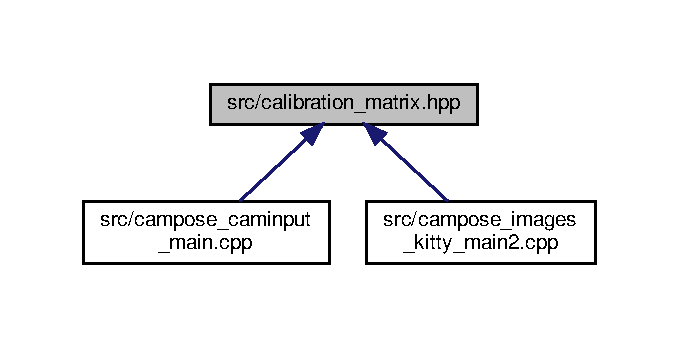
\includegraphics[width=326pt]{calibration__matrix_8hpp__dep__incl}
\end{center}
\end{figure}
\subsection*{Variables}
\begin{DoxyCompactItemize}
\item 
float \hyperlink{calibration__matrix_8hpp_a402a49abec31f401cd3ddea778e35267}{calib\+\_\+elem} \mbox{[}9\mbox{]} = \{ 721.\+5377, 0, 609.\+5593, 0, 721.\+5377, 172.\+854, 0, 0, 1 \}
\item 
cv\+::\+Mat \hyperlink{calibration__matrix_8hpp_a7a1efed611ca1c58941312f1f2332694}{A\+\_\+calib} = cv\+::\+Mat(3, 3, C\+V\+\_\+32F, \hyperlink{calibration__matrix_8hpp_a402a49abec31f401cd3ddea778e35267}{calib\+\_\+elem})
\item 
float \hyperlink{calibration__matrix_8hpp_a6ac9c62aefb64584875c504b5e18d515}{distortion\+\_\+elem} \mbox{[}14\mbox{]} = \{ 0, 0, 0, 0, 0, 0, 0, 0, 0, 0, 0, 0, 0, 0\}
\item 
cv\+::\+Mat \hyperlink{calibration__matrix_8hpp_ade1f7415a2c3909efea478507e6f8e62}{D\+\_\+calib} = cv\+::\+Mat(1, 14, C\+V\+\_\+32F, \hyperlink{calibration__matrix_8hpp_a6ac9c62aefb64584875c504b5e18d515}{distortion\+\_\+elem})
\end{DoxyCompactItemize}


\subsection{Variable Documentation}
\mbox{\Hypertarget{calibration__matrix_8hpp_a7a1efed611ca1c58941312f1f2332694}\label{calibration__matrix_8hpp_a7a1efed611ca1c58941312f1f2332694}} 
\index{calibration\+\_\+matrix.\+hpp@{calibration\+\_\+matrix.\+hpp}!A\+\_\+calib@{A\+\_\+calib}}
\index{A\+\_\+calib@{A\+\_\+calib}!calibration\+\_\+matrix.\+hpp@{calibration\+\_\+matrix.\+hpp}}
\subsubsection{\texorpdfstring{A\+\_\+calib}{A\_calib}}
{\footnotesize\ttfamily cv\+::\+Mat A\+\_\+calib = cv\+::\+Mat(3, 3, C\+V\+\_\+32F, \hyperlink{calibration__matrix_8hpp_a402a49abec31f401cd3ddea778e35267}{calib\+\_\+elem})}

\mbox{\Hypertarget{calibration__matrix_8hpp_a402a49abec31f401cd3ddea778e35267}\label{calibration__matrix_8hpp_a402a49abec31f401cd3ddea778e35267}} 
\index{calibration\+\_\+matrix.\+hpp@{calibration\+\_\+matrix.\+hpp}!calib\+\_\+elem@{calib\+\_\+elem}}
\index{calib\+\_\+elem@{calib\+\_\+elem}!calibration\+\_\+matrix.\+hpp@{calibration\+\_\+matrix.\+hpp}}
\subsubsection{\texorpdfstring{calib\+\_\+elem}{calib\_elem}}
{\footnotesize\ttfamily float calib\+\_\+elem\mbox{[}9\mbox{]} = \{ 721.\+5377, 0, 609.\+5593, 0, 721.\+5377, 172.\+854, 0, 0, 1 \}}

\mbox{\Hypertarget{calibration__matrix_8hpp_ade1f7415a2c3909efea478507e6f8e62}\label{calibration__matrix_8hpp_ade1f7415a2c3909efea478507e6f8e62}} 
\index{calibration\+\_\+matrix.\+hpp@{calibration\+\_\+matrix.\+hpp}!D\+\_\+calib@{D\+\_\+calib}}
\index{D\+\_\+calib@{D\+\_\+calib}!calibration\+\_\+matrix.\+hpp@{calibration\+\_\+matrix.\+hpp}}
\subsubsection{\texorpdfstring{D\+\_\+calib}{D\_calib}}
{\footnotesize\ttfamily cv\+::\+Mat D\+\_\+calib = cv\+::\+Mat(1, 14, C\+V\+\_\+32F, \hyperlink{calibration__matrix_8hpp_a6ac9c62aefb64584875c504b5e18d515}{distortion\+\_\+elem})}

\mbox{\Hypertarget{calibration__matrix_8hpp_a6ac9c62aefb64584875c504b5e18d515}\label{calibration__matrix_8hpp_a6ac9c62aefb64584875c504b5e18d515}} 
\index{calibration\+\_\+matrix.\+hpp@{calibration\+\_\+matrix.\+hpp}!distortion\+\_\+elem@{distortion\+\_\+elem}}
\index{distortion\+\_\+elem@{distortion\+\_\+elem}!calibration\+\_\+matrix.\+hpp@{calibration\+\_\+matrix.\+hpp}}
\subsubsection{\texorpdfstring{distortion\+\_\+elem}{distortion\_elem}}
{\footnotesize\ttfamily float distortion\+\_\+elem\mbox{[}14\mbox{]} = \{ 0, 0, 0, 0, 0, 0, 0, 0, 0, 0, 0, 0, 0, 0\}}


\hypertarget{campose__caminput__main_8cpp}{}\section{src/campose\+\_\+caminput\+\_\+main.cpp File Reference}
\label{campose__caminput__main_8cpp}\index{src/campose\+\_\+caminput\+\_\+main.\+cpp@{src/campose\+\_\+caminput\+\_\+main.\+cpp}}
{\ttfamily \#include $<$opencv2/core.\+hpp$>$}\newline
{\ttfamily \#include $<$opencv2/imgcodecs.\+hpp$>$}\newline
{\ttfamily \#include $<$opencv2/highgui.\+hpp$>$}\newline
{\ttfamily \#include $<$opencv2/viz.\+hpp$>$}\newline
{\ttfamily \#include $<$iostream$>$}\newline
{\ttfamily \#include $<$boost/circular\+\_\+buffer.\+hpp$>$}\newline
{\ttfamily \#include \char`\"{}calibration\+\_\+matrix.\+hpp\char`\"{}}\newline
{\ttfamily \#include \char`\"{}data\+Structures.\+h\char`\"{}}\newline
{\ttfamily \#include \char`\"{}Keypoint\+Processor\+Gpu.\+hpp\char`\"{}}\newline
{\ttfamily \#include \char`\"{}Camera\+Pose\+Estimator.\+hpp\char`\"{}}\newline
Include dependency graph for campose\+\_\+caminput\+\_\+main.\+cpp\+:\nopagebreak
\begin{figure}[H]
\begin{center}
\leavevmode
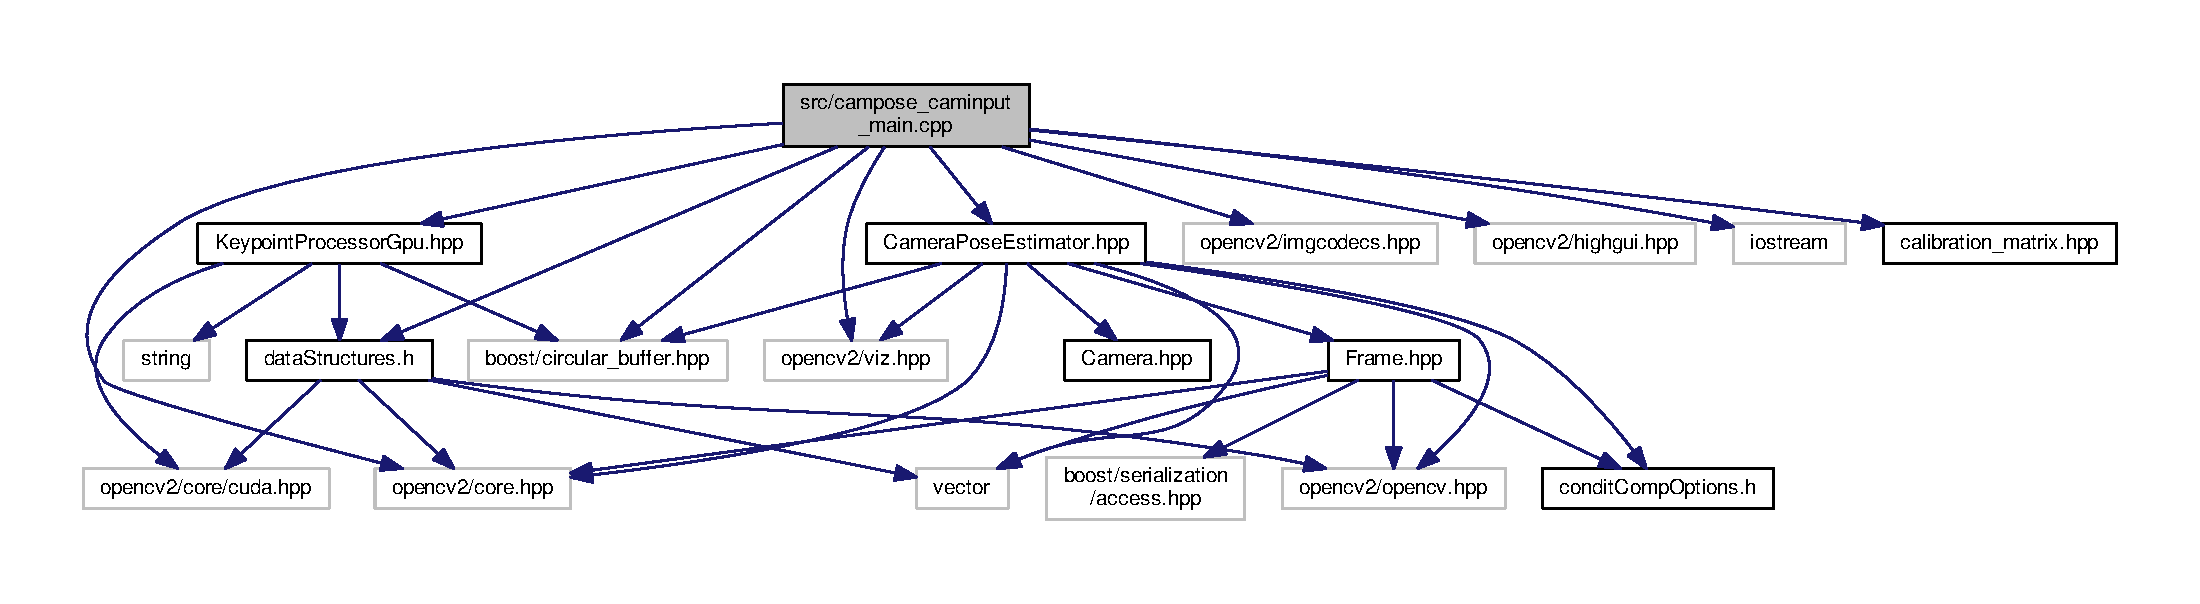
\includegraphics[width=350pt]{campose__caminput__main_8cpp__incl}
\end{center}
\end{figure}
\subsection*{Functions}
\begin{DoxyCompactItemize}
\item 
int \hyperlink{campose__caminput__main_8cpp_a6c9ea8b891fe570df90a82d6d3741244}{show\+Camera\+Raw} (cv\+::\+Mat \&cam\+Frame)
\item 
int \hyperlink{campose__caminput__main_8cpp_a84cd556aac30a8e98bf9a5eb581cc139}{get\+Camera\+Fw\+Left} (cv\+::\+Mat $\ast$cam\+Frame, cv\+::\+Mat $\ast$cam\+Fw\+Left\+Frame)
\item 
int \hyperlink{campose__caminput__main_8cpp_adeece51f161493d2eb11c4165d4ac5f2}{get\+Camera\+Fw\+Right} (cv\+::\+Mat $\ast$cam\+Frame, cv\+::\+Mat $\ast$cam\+Fw\+Right\+Frame)
\item 
int \hyperlink{campose__caminput__main_8cpp_a3c04138a5bfe5d72780bb7e82a18e627}{main} (int argc, char $\ast$$\ast$argv)
\end{DoxyCompactItemize}


\subsection{Function Documentation}
\mbox{\Hypertarget{campose__caminput__main_8cpp_a84cd556aac30a8e98bf9a5eb581cc139}\label{campose__caminput__main_8cpp_a84cd556aac30a8e98bf9a5eb581cc139}} 
\index{campose\+\_\+caminput\+\_\+main.\+cpp@{campose\+\_\+caminput\+\_\+main.\+cpp}!get\+Camera\+Fw\+Left@{get\+Camera\+Fw\+Left}}
\index{get\+Camera\+Fw\+Left@{get\+Camera\+Fw\+Left}!campose\+\_\+caminput\+\_\+main.\+cpp@{campose\+\_\+caminput\+\_\+main.\+cpp}}
\subsubsection{\texorpdfstring{get\+Camera\+Fw\+Left()}{getCameraFwLeft()}}
{\footnotesize\ttfamily int get\+Camera\+Fw\+Left (\begin{DoxyParamCaption}\item[{cv\+::\+Mat $\ast$}]{cam\+Frame,  }\item[{cv\+::\+Mat $\ast$}]{cam\+Fw\+Left\+Frame }\end{DoxyParamCaption})}

\mbox{\Hypertarget{campose__caminput__main_8cpp_adeece51f161493d2eb11c4165d4ac5f2}\label{campose__caminput__main_8cpp_adeece51f161493d2eb11c4165d4ac5f2}} 
\index{campose\+\_\+caminput\+\_\+main.\+cpp@{campose\+\_\+caminput\+\_\+main.\+cpp}!get\+Camera\+Fw\+Right@{get\+Camera\+Fw\+Right}}
\index{get\+Camera\+Fw\+Right@{get\+Camera\+Fw\+Right}!campose\+\_\+caminput\+\_\+main.\+cpp@{campose\+\_\+caminput\+\_\+main.\+cpp}}
\subsubsection{\texorpdfstring{get\+Camera\+Fw\+Right()}{getCameraFwRight()}}
{\footnotesize\ttfamily int get\+Camera\+Fw\+Right (\begin{DoxyParamCaption}\item[{cv\+::\+Mat $\ast$}]{cam\+Frame,  }\item[{cv\+::\+Mat $\ast$}]{cam\+Fw\+Right\+Frame }\end{DoxyParamCaption})}

\mbox{\Hypertarget{campose__caminput__main_8cpp_a3c04138a5bfe5d72780bb7e82a18e627}\label{campose__caminput__main_8cpp_a3c04138a5bfe5d72780bb7e82a18e627}} 
\index{campose\+\_\+caminput\+\_\+main.\+cpp@{campose\+\_\+caminput\+\_\+main.\+cpp}!main@{main}}
\index{main@{main}!campose\+\_\+caminput\+\_\+main.\+cpp@{campose\+\_\+caminput\+\_\+main.\+cpp}}
\subsubsection{\texorpdfstring{main()}{main()}}
{\footnotesize\ttfamily int main (\begin{DoxyParamCaption}\item[{int}]{argc,  }\item[{char $\ast$$\ast$}]{argv }\end{DoxyParamCaption})}

Here is the call graph for this function\+:\nopagebreak
\begin{figure}[H]
\begin{center}
\leavevmode
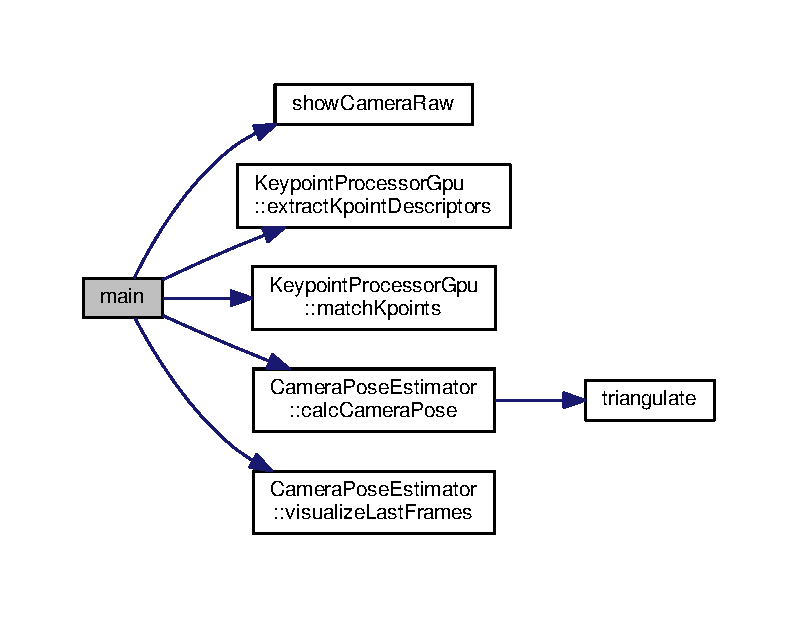
\includegraphics[width=350pt]{campose__caminput__main_8cpp_a3c04138a5bfe5d72780bb7e82a18e627_cgraph}
\end{center}
\end{figure}
\mbox{\Hypertarget{campose__caminput__main_8cpp_a6c9ea8b891fe570df90a82d6d3741244}\label{campose__caminput__main_8cpp_a6c9ea8b891fe570df90a82d6d3741244}} 
\index{campose\+\_\+caminput\+\_\+main.\+cpp@{campose\+\_\+caminput\+\_\+main.\+cpp}!show\+Camera\+Raw@{show\+Camera\+Raw}}
\index{show\+Camera\+Raw@{show\+Camera\+Raw}!campose\+\_\+caminput\+\_\+main.\+cpp@{campose\+\_\+caminput\+\_\+main.\+cpp}}
\subsubsection{\texorpdfstring{show\+Camera\+Raw()}{showCameraRaw()}}
{\footnotesize\ttfamily int show\+Camera\+Raw (\begin{DoxyParamCaption}\item[{cv\+::\+Mat \&}]{cam\+Frame }\end{DoxyParamCaption})}

Here is the caller graph for this function\+:\nopagebreak
\begin{figure}[H]
\begin{center}
\leavevmode
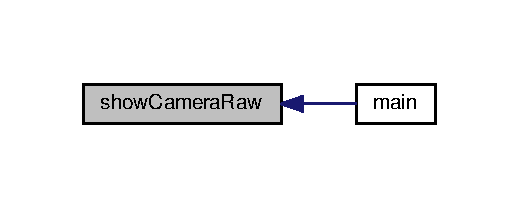
\includegraphics[width=249pt]{campose__caminput__main_8cpp_a6c9ea8b891fe570df90a82d6d3741244_icgraph}
\end{center}
\end{figure}

\hypertarget{campose__images__kitty__main2_8cpp}{}\section{src/campose\+\_\+images\+\_\+kitty\+\_\+main2.cpp File Reference}
\label{campose__images__kitty__main2_8cpp}\index{src/campose\+\_\+images\+\_\+kitty\+\_\+main2.\+cpp@{src/campose\+\_\+images\+\_\+kitty\+\_\+main2.\+cpp}}
{\ttfamily \#include $<$opencv2/core.\+hpp$>$}\\*
{\ttfamily \#include $<$opencv2/imgcodecs.\+hpp$>$}\\*
{\ttfamily \#include $<$opencv2/highgui.\+hpp$>$}\\*
{\ttfamily \#include $<$opencv2/viz.\+hpp$>$}\\*
{\ttfamily \#include $<$iostream$>$}\\*
{\ttfamily \#include $<$boost/circular\+\_\+buffer.\+hpp$>$}\\*
{\ttfamily \#include $<$thread$>$}\\*
{\ttfamily \#include $<$mutex$>$}\\*
{\ttfamily \#include $<$memory$>$}\\*
{\ttfamily \#include \char`\"{}calibration\+\_\+matrix.\+hpp\char`\"{}}\\*
{\ttfamily \#include \char`\"{}Kpoint\+Processor.\+hpp\char`\"{}}\\*
{\ttfamily \#include \char`\"{}Camera\+Pose\+Estimator.\+hpp\char`\"{}}\\*
{\ttfamily \#include \char`\"{}Frame\+Provider.\+hpp\char`\"{}}\\*
Include dependency graph for campose\+\_\+images\+\_\+kitty\+\_\+main2.\+cpp\+:
\nopagebreak
\begin{figure}[H]
\begin{center}
\leavevmode
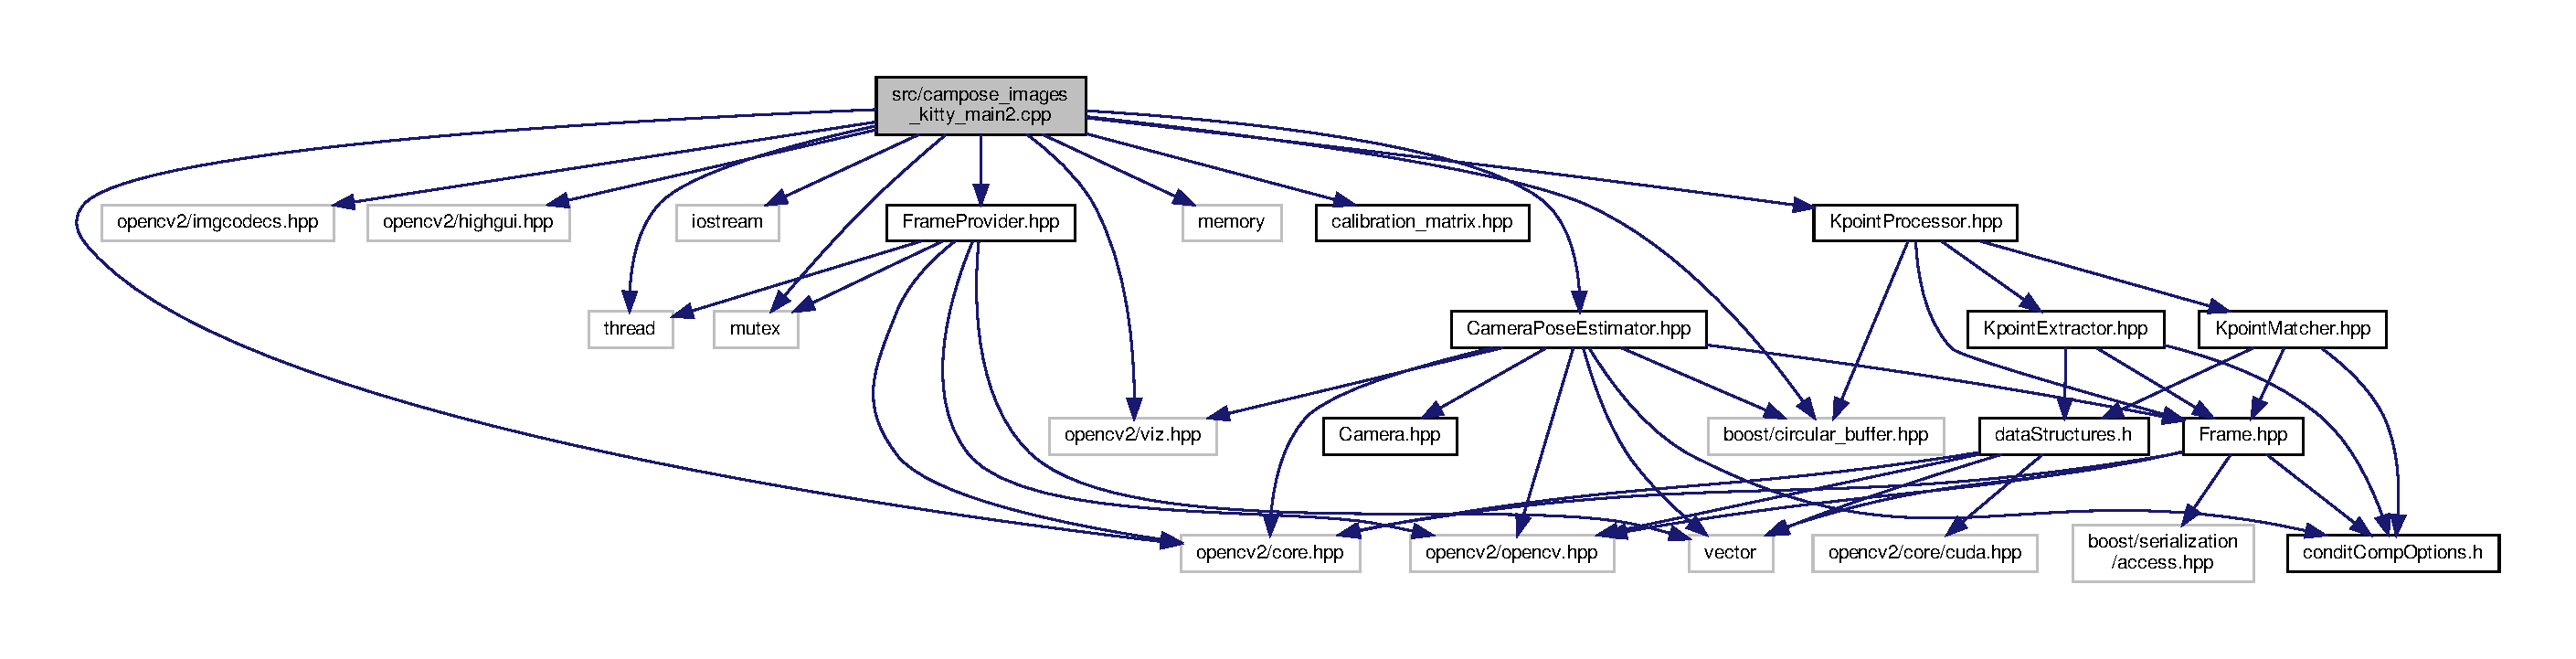
\includegraphics[width=350pt]{campose__images__kitty__main2_8cpp__incl}
\end{center}
\end{figure}
\subsection*{Functions}
\begin{DoxyCompactItemize}
\item 
int \hyperlink{campose__images__kitty__main2_8cpp_a6c9ea8b891fe570df90a82d6d3741244}{show\+Camera\+Raw} (cv\+::\+Mat \&cam\+Frame)
\item 
int \hyperlink{campose__images__kitty__main2_8cpp_aea0169e6cd467049d7ff7db330281eb7}{show\+Image\+Raw} (cv\+::\+Mat \&image\+Frame, double fps\+\_\+processing)
\item 
int \hyperlink{campose__images__kitty__main2_8cpp_a3c04138a5bfe5d72780bb7e82a18e627}{main} (int argc, char $\ast$$\ast$argv)
\end{DoxyCompactItemize}
\subsection*{Variables}
\begin{DoxyCompactItemize}
\item 
cv\+::\+Mat \hyperlink{campose__images__kitty__main2_8cpp_a5e086ff818c928d0c04841b868cb7cfd}{global\+Frame}
\item 
mutex \hyperlink{campose__images__kitty__main2_8cpp_a29ac681ec3efa9e30e1ab1ab251b47f9}{mtx}
\item 
bool \hyperlink{campose__images__kitty__main2_8cpp_a1d84dbc32fc3d19979c84da744fa83ab}{frame\+Available} = false
\end{DoxyCompactItemize}


\subsection{Function Documentation}
\index{campose\+\_\+images\+\_\+kitty\+\_\+main2.\+cpp@{campose\+\_\+images\+\_\+kitty\+\_\+main2.\+cpp}!main@{main}}
\index{main@{main}!campose\+\_\+images\+\_\+kitty\+\_\+main2.\+cpp@{campose\+\_\+images\+\_\+kitty\+\_\+main2.\+cpp}}
\subsubsection[{\texorpdfstring{main(int argc, char $\ast$$\ast$argv)}{main(int argc, char **argv)}}]{\setlength{\rightskip}{0pt plus 5cm}int main (
\begin{DoxyParamCaption}
\item[{int}]{argc, }
\item[{char $\ast$$\ast$}]{argv}
\end{DoxyParamCaption}
)}\hypertarget{campose__images__kitty__main2_8cpp_a3c04138a5bfe5d72780bb7e82a18e627}{}\label{campose__images__kitty__main2_8cpp_a3c04138a5bfe5d72780bb7e82a18e627}


Here is the call graph for this function\+:
\nopagebreak
\begin{figure}[H]
\begin{center}
\leavevmode
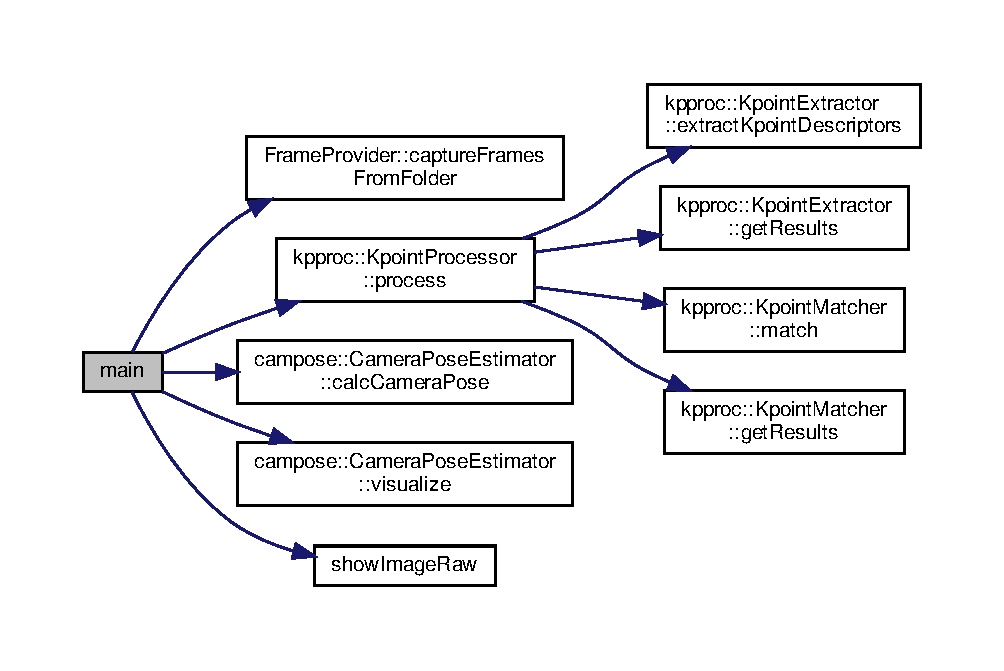
\includegraphics[width=350pt]{campose__images__kitty__main2_8cpp_a3c04138a5bfe5d72780bb7e82a18e627_cgraph}
\end{center}
\end{figure}


\index{campose\+\_\+images\+\_\+kitty\+\_\+main2.\+cpp@{campose\+\_\+images\+\_\+kitty\+\_\+main2.\+cpp}!show\+Camera\+Raw@{show\+Camera\+Raw}}
\index{show\+Camera\+Raw@{show\+Camera\+Raw}!campose\+\_\+images\+\_\+kitty\+\_\+main2.\+cpp@{campose\+\_\+images\+\_\+kitty\+\_\+main2.\+cpp}}
\subsubsection[{\texorpdfstring{show\+Camera\+Raw(cv\+::\+Mat \&cam\+Frame)}{showCameraRaw(cv::Mat &camFrame)}}]{\setlength{\rightskip}{0pt plus 5cm}int show\+Camera\+Raw (
\begin{DoxyParamCaption}
\item[{cv\+::\+Mat \&}]{cam\+Frame}
\end{DoxyParamCaption}
)}\hypertarget{campose__images__kitty__main2_8cpp_a6c9ea8b891fe570df90a82d6d3741244}{}\label{campose__images__kitty__main2_8cpp_a6c9ea8b891fe570df90a82d6d3741244}
\index{campose\+\_\+images\+\_\+kitty\+\_\+main2.\+cpp@{campose\+\_\+images\+\_\+kitty\+\_\+main2.\+cpp}!show\+Image\+Raw@{show\+Image\+Raw}}
\index{show\+Image\+Raw@{show\+Image\+Raw}!campose\+\_\+images\+\_\+kitty\+\_\+main2.\+cpp@{campose\+\_\+images\+\_\+kitty\+\_\+main2.\+cpp}}
\subsubsection[{\texorpdfstring{show\+Image\+Raw(cv\+::\+Mat \&image\+Frame, double fps\+\_\+processing)}{showImageRaw(cv::Mat &imageFrame, double fps_processing)}}]{\setlength{\rightskip}{0pt plus 5cm}int show\+Image\+Raw (
\begin{DoxyParamCaption}
\item[{cv\+::\+Mat \&}]{image\+Frame, }
\item[{double}]{fps\+\_\+processing}
\end{DoxyParamCaption}
)}\hypertarget{campose__images__kitty__main2_8cpp_aea0169e6cd467049d7ff7db330281eb7}{}\label{campose__images__kitty__main2_8cpp_aea0169e6cd467049d7ff7db330281eb7}


Here is the caller graph for this function\+:\nopagebreak
\begin{figure}[H]
\begin{center}
\leavevmode
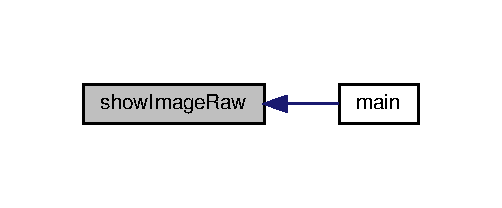
\includegraphics[width=241pt]{campose__images__kitty__main2_8cpp_aea0169e6cd467049d7ff7db330281eb7_icgraph}
\end{center}
\end{figure}




\subsection{Variable Documentation}
\index{campose\+\_\+images\+\_\+kitty\+\_\+main2.\+cpp@{campose\+\_\+images\+\_\+kitty\+\_\+main2.\+cpp}!frame\+Available@{frame\+Available}}
\index{frame\+Available@{frame\+Available}!campose\+\_\+images\+\_\+kitty\+\_\+main2.\+cpp@{campose\+\_\+images\+\_\+kitty\+\_\+main2.\+cpp}}
\subsubsection[{\texorpdfstring{frame\+Available}{frameAvailable}}]{\setlength{\rightskip}{0pt plus 5cm}bool frame\+Available = false}\hypertarget{campose__images__kitty__main2_8cpp_a1d84dbc32fc3d19979c84da744fa83ab}{}\label{campose__images__kitty__main2_8cpp_a1d84dbc32fc3d19979c84da744fa83ab}
\index{campose\+\_\+images\+\_\+kitty\+\_\+main2.\+cpp@{campose\+\_\+images\+\_\+kitty\+\_\+main2.\+cpp}!global\+Frame@{global\+Frame}}
\index{global\+Frame@{global\+Frame}!campose\+\_\+images\+\_\+kitty\+\_\+main2.\+cpp@{campose\+\_\+images\+\_\+kitty\+\_\+main2.\+cpp}}
\subsubsection[{\texorpdfstring{global\+Frame}{globalFrame}}]{\setlength{\rightskip}{0pt plus 5cm}cv\+::\+Mat global\+Frame}\hypertarget{campose__images__kitty__main2_8cpp_a5e086ff818c928d0c04841b868cb7cfd}{}\label{campose__images__kitty__main2_8cpp_a5e086ff818c928d0c04841b868cb7cfd}
\index{campose\+\_\+images\+\_\+kitty\+\_\+main2.\+cpp@{campose\+\_\+images\+\_\+kitty\+\_\+main2.\+cpp}!mtx@{mtx}}
\index{mtx@{mtx}!campose\+\_\+images\+\_\+kitty\+\_\+main2.\+cpp@{campose\+\_\+images\+\_\+kitty\+\_\+main2.\+cpp}}
\subsubsection[{\texorpdfstring{mtx}{mtx}}]{\setlength{\rightskip}{0pt plus 5cm}mutex mtx}\hypertarget{campose__images__kitty__main2_8cpp_a29ac681ec3efa9e30e1ab1ab251b47f9}{}\label{campose__images__kitty__main2_8cpp_a29ac681ec3efa9e30e1ab1ab251b47f9}

\hypertarget{Camera_8hpp}{}\section{src/frame/\+Camera.hpp File Reference}
\label{Camera_8hpp}\index{src/frame/\+Camera.\+hpp@{src/frame/\+Camera.\+hpp}}
This graph shows which files directly or indirectly include this file\+:\nopagebreak
\begin{figure}[H]
\begin{center}
\leavevmode
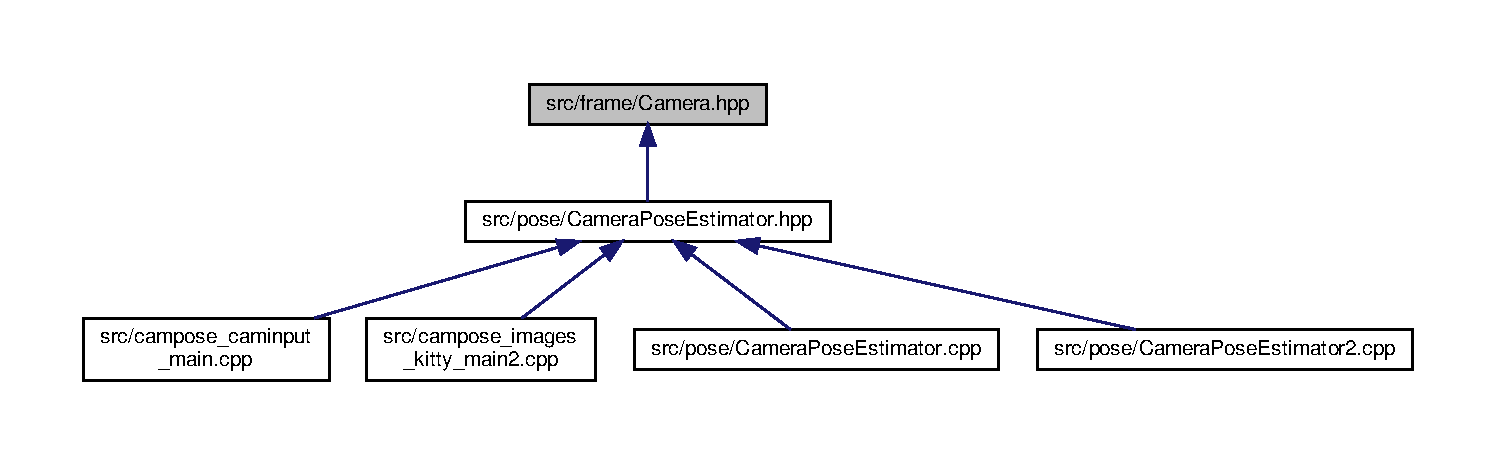
\includegraphics[width=350pt]{Camera_8hpp__dep__incl}
\end{center}
\end{figure}
\subsection*{Classes}
\begin{DoxyCompactItemize}
\item 
class \hyperlink{classCamera}{Camera}
\end{DoxyCompactItemize}

\hypertarget{dataStructures_8h}{}\section{src/frame/data\+Structures.h File Reference}
\label{dataStructures_8h}\index{src/frame/data\+Structures.\+h@{src/frame/data\+Structures.\+h}}
{\ttfamily \#include $<$vector$>$}\\*
{\ttfamily \#include $<$opencv2/core.\+hpp$>$}\\*
{\ttfamily \#include \char`\"{}opencv2/opencv.\+hpp\char`\"{}}\\*
{\ttfamily \#include $<$opencv2/core/cuda.\+hpp$>$}\\*
Include dependency graph for data\+Structures.\+h\+:\nopagebreak
\begin{figure}[H]
\begin{center}
\leavevmode
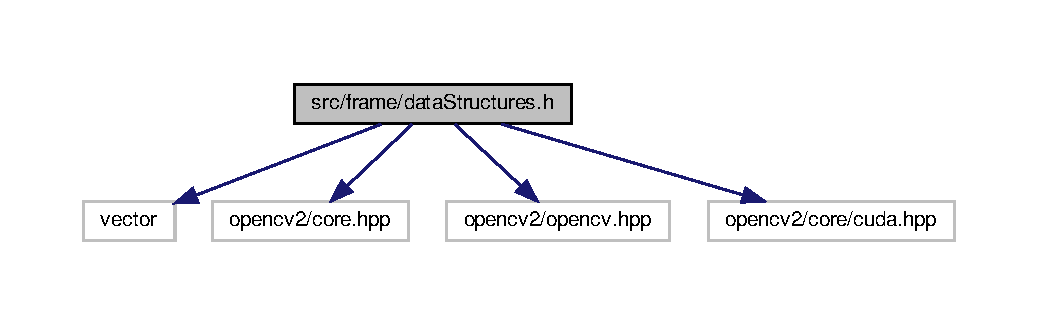
\includegraphics[width=350pt]{dataStructures_8h__incl}
\end{center}
\end{figure}
This graph shows which files directly or indirectly include this file\+:
\nopagebreak
\begin{figure}[H]
\begin{center}
\leavevmode
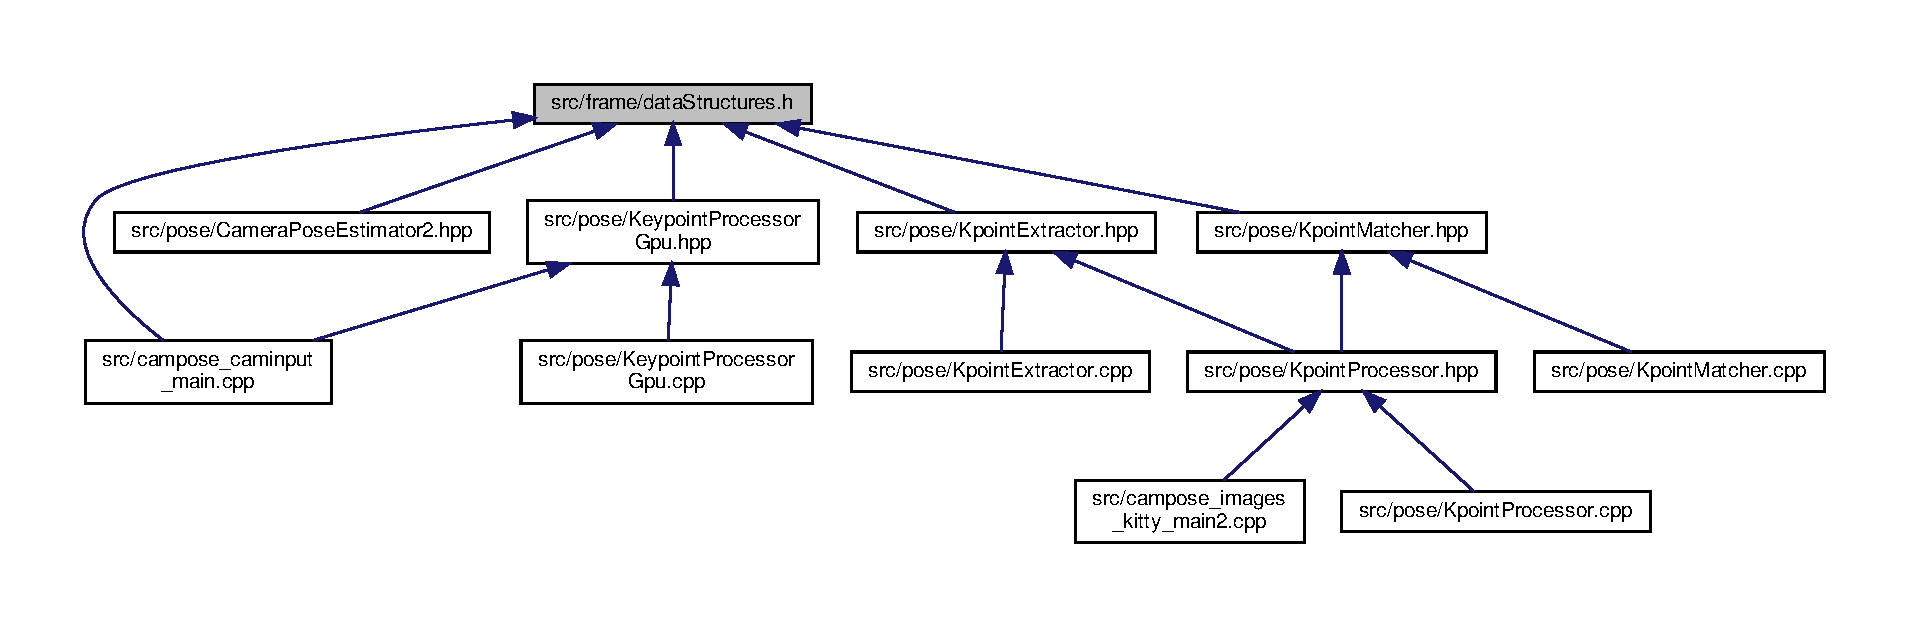
\includegraphics[width=350pt]{dataStructures_8h__dep__incl}
\end{center}
\end{figure}
\subsection*{Classes}
\begin{DoxyCompactItemize}
\item 
struct \hyperlink{structDataFrame}{Data\+Frame}
\end{DoxyCompactItemize}

\hypertarget{Frame_8hpp}{}\section{src/frame/\+Frame.hpp File Reference}
\label{Frame_8hpp}\index{src/frame/\+Frame.\+hpp@{src/frame/\+Frame.\+hpp}}
{\ttfamily \#include $<$vector$>$}\\*
{\ttfamily \#include $<$opencv2/core.\+hpp$>$}\\*
{\ttfamily \#include \char`\"{}opencv2/opencv.\+hpp\char`\"{}}\\*
{\ttfamily \#include $<$boost/serialization/access.\+hpp$>$}\\*
{\ttfamily \#include \char`\"{}condit\+Comp\+Options.\+h\char`\"{}}\\*
Include dependency graph for Frame.\+hpp\+:\nopagebreak
\begin{figure}[H]
\begin{center}
\leavevmode
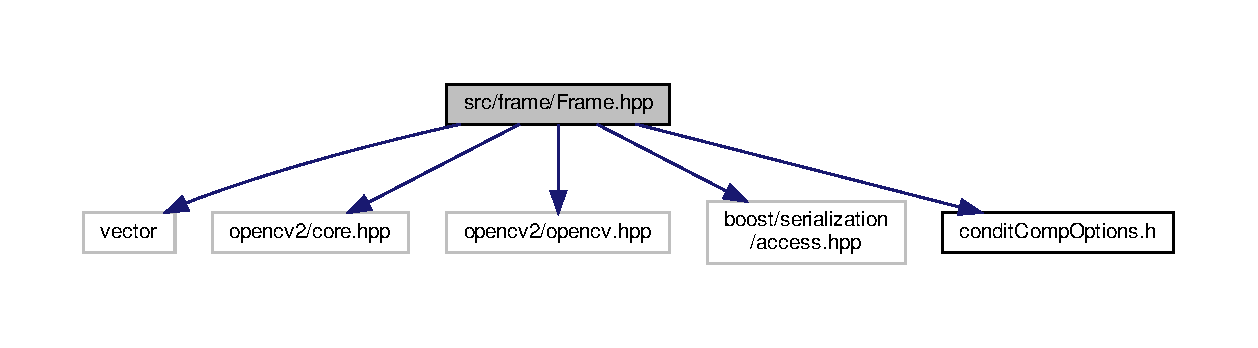
\includegraphics[width=350pt]{Frame_8hpp__incl}
\end{center}
\end{figure}
This graph shows which files directly or indirectly include this file\+:
\nopagebreak
\begin{figure}[H]
\begin{center}
\leavevmode
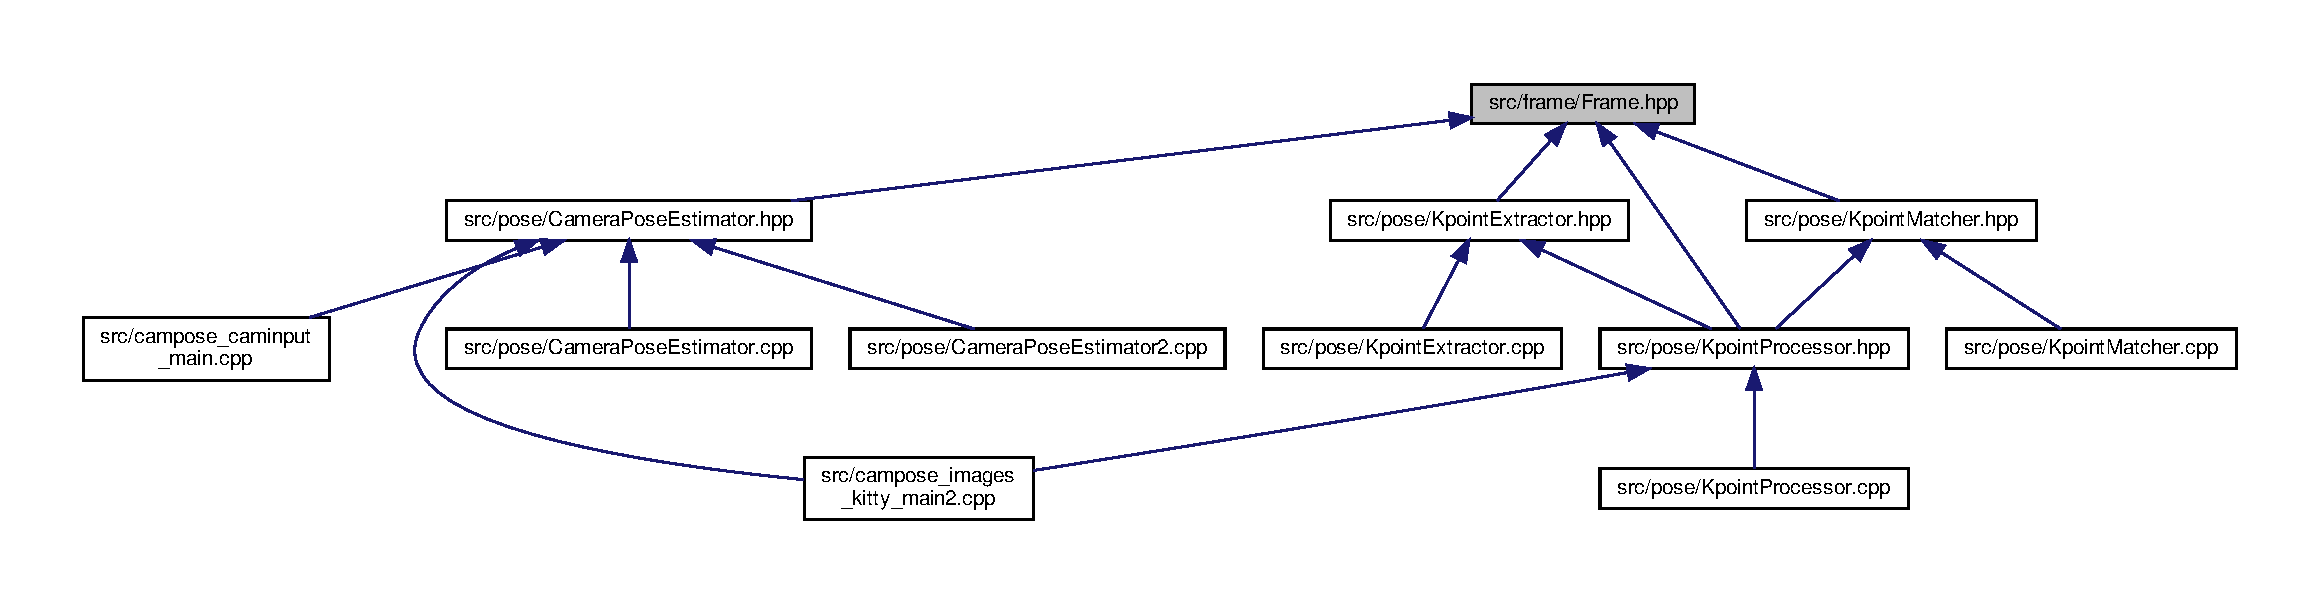
\includegraphics[width=350pt]{Frame_8hpp__dep__incl}
\end{center}
\end{figure}
\subsection*{Classes}
\begin{DoxyCompactItemize}
\item 
class \hyperlink{classFrame}{Frame}
\end{DoxyCompactItemize}

\hypertarget{FrameProvider_8cpp}{}\section{src/frame/\+Frame\+Provider.cpp File Reference}
\label{FrameProvider_8cpp}\index{src/frame/\+Frame\+Provider.\+cpp@{src/frame/\+Frame\+Provider.\+cpp}}
{\ttfamily \#include \char`\"{}Frame\+Provider.\+hpp\char`\"{}}\newline
{\ttfamily \#include $<$unistd.\+h$>$}\newline
Include dependency graph for Frame\+Provider.\+cpp\+:\nopagebreak
\begin{figure}[H]
\begin{center}
\leavevmode
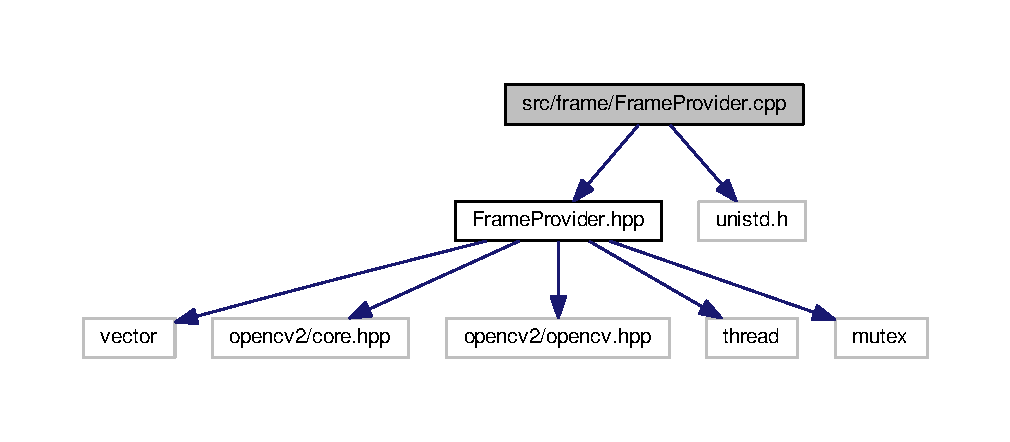
\includegraphics[width=350pt]{FrameProvider_8cpp__incl}
\end{center}
\end{figure}

\hypertarget{FrameProvider_8hpp}{}\section{src/frame/\+Frame\+Provider.hpp File Reference}
\label{FrameProvider_8hpp}\index{src/frame/\+Frame\+Provider.\+hpp@{src/frame/\+Frame\+Provider.\+hpp}}
{\ttfamily \#include $<$vector$>$}\\*
{\ttfamily \#include $<$opencv2/core.\+hpp$>$}\\*
{\ttfamily \#include \char`\"{}opencv2/opencv.\+hpp\char`\"{}}\\*
{\ttfamily \#include $<$thread$>$}\\*
{\ttfamily \#include $<$mutex$>$}\\*
Include dependency graph for Frame\+Provider.\+hpp\+:\nopagebreak
\begin{figure}[H]
\begin{center}
\leavevmode
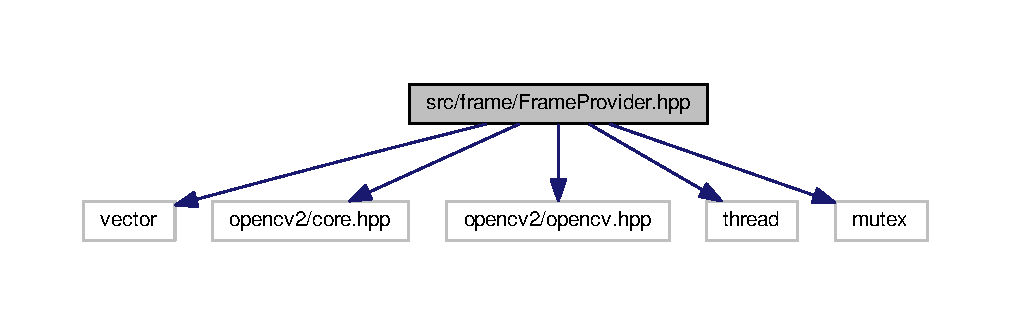
\includegraphics[width=350pt]{FrameProvider_8hpp__incl}
\end{center}
\end{figure}
This graph shows which files directly or indirectly include this file\+:\nopagebreak
\begin{figure}[H]
\begin{center}
\leavevmode
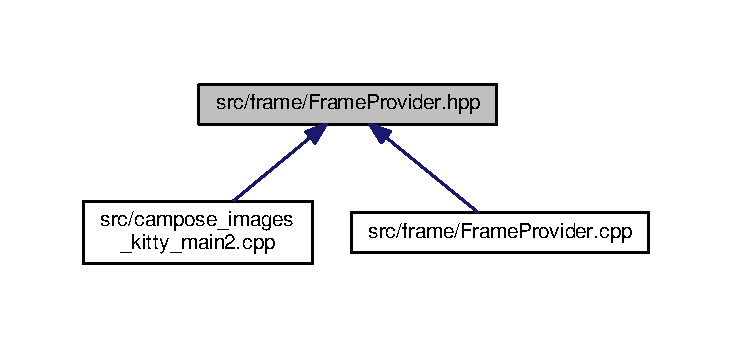
\includegraphics[width=350pt]{FrameProvider_8hpp__dep__incl}
\end{center}
\end{figure}
\subsection*{Classes}
\begin{DoxyCompactItemize}
\item 
class \hyperlink{classFrameProvider}{Frame\+Provider}
\end{DoxyCompactItemize}

\hypertarget{CameraPoseEstimator_8cpp}{}\section{src/pose/\+Camera\+Pose\+Estimator.cpp File Reference}
\label{CameraPoseEstimator_8cpp}\index{src/pose/\+Camera\+Pose\+Estimator.\+cpp@{src/pose/\+Camera\+Pose\+Estimator.\+cpp}}
{\ttfamily \#include \char`\"{}Camera\+Pose\+Estimator.\+hpp\char`\"{}}\\*
{\ttfamily \#include $<$string$>$}\\*
{\ttfamily \#include $<$iostream$>$}\\*
{\ttfamily \#include \char`\"{}opencv2/calib3d.\+hpp\char`\"{}}\\*
{\ttfamily \#include $<$opencv2/viz.\+hpp$>$}\\*
{\ttfamily \#include $<$opencv2/viz/widgets.\+hpp$>$}\\*
{\ttfamily \#include $<$opencv2/core/types.\+hpp$>$}\\*
Include dependency graph for Camera\+Pose\+Estimator.\+cpp\+:\nopagebreak
\begin{figure}[H]
\begin{center}
\leavevmode
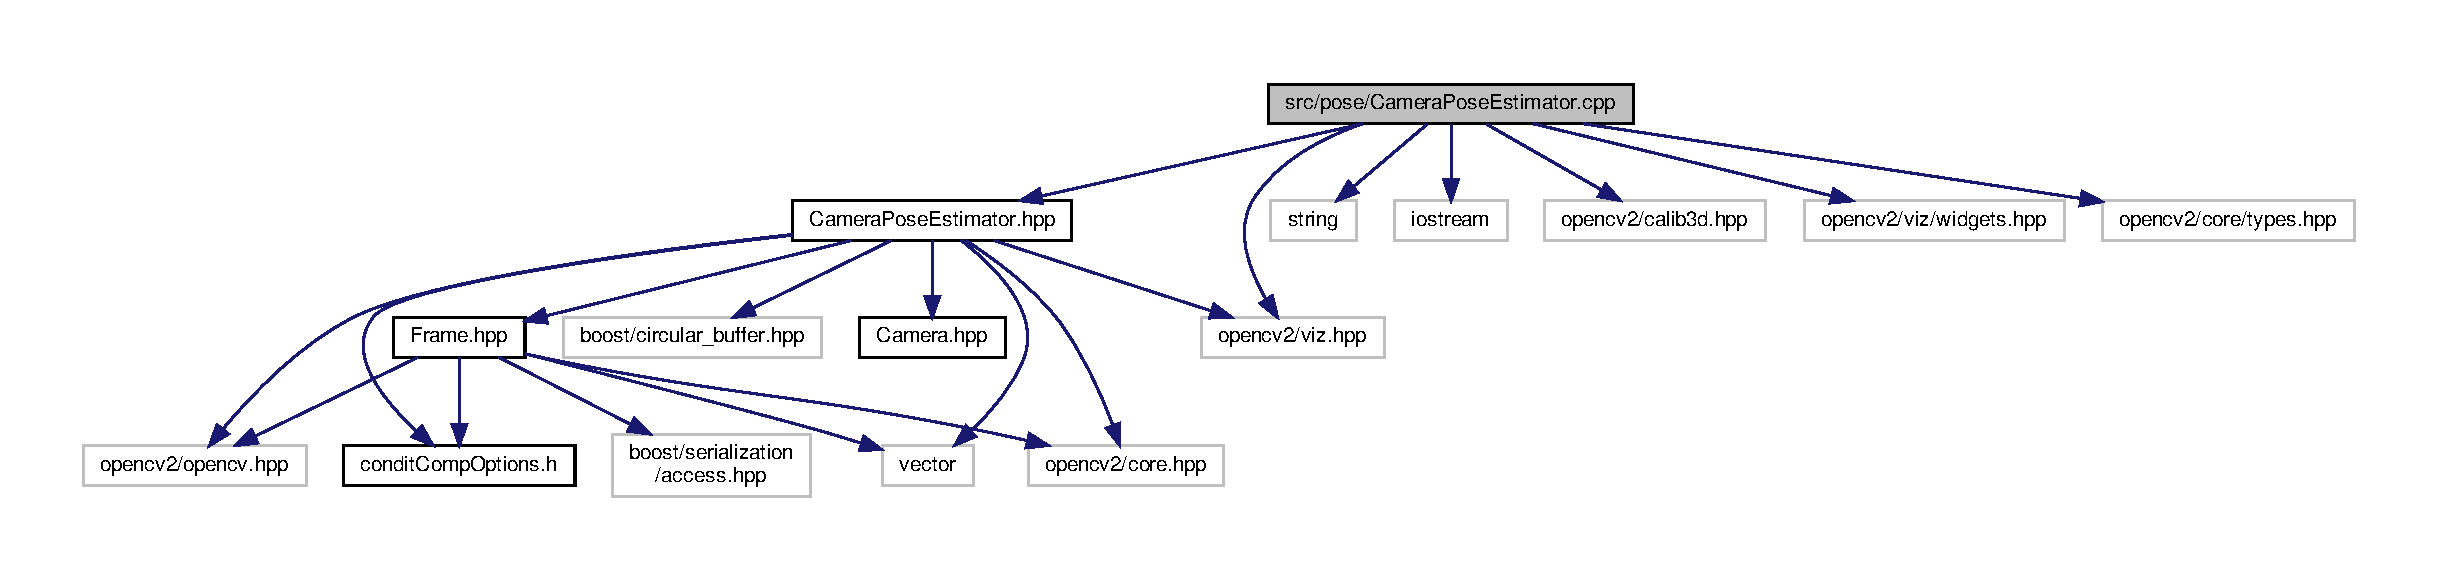
\includegraphics[width=350pt]{CameraPoseEstimator_8cpp__incl}
\end{center}
\end{figure}

\hypertarget{CameraPoseEstimator_8hpp}{}\section{src/pose/\+Camera\+Pose\+Estimator.hpp File Reference}
\label{CameraPoseEstimator_8hpp}\index{src/pose/\+Camera\+Pose\+Estimator.\+hpp@{src/pose/\+Camera\+Pose\+Estimator.\+hpp}}
{\ttfamily \#include $<$vector$>$}\\*
{\ttfamily \#include $<$opencv2/core.\+hpp$>$}\\*
{\ttfamily \#include \char`\"{}opencv2/opencv.\+hpp\char`\"{}}\\*
{\ttfamily \#include $<$boost/circular\+\_\+buffer.\+hpp$>$}\\*
{\ttfamily \#include $<$opencv2/viz.\+hpp$>$}\\*
{\ttfamily \#include \char`\"{}Camera.\+hpp\char`\"{}}\\*
{\ttfamily \#include \char`\"{}condit\+Comp\+Options.\+h\char`\"{}}\\*
{\ttfamily \#include \char`\"{}Frame.\+hpp\char`\"{}}\\*
Include dependency graph for Camera\+Pose\+Estimator.\+hpp\+:\nopagebreak
\begin{figure}[H]
\begin{center}
\leavevmode
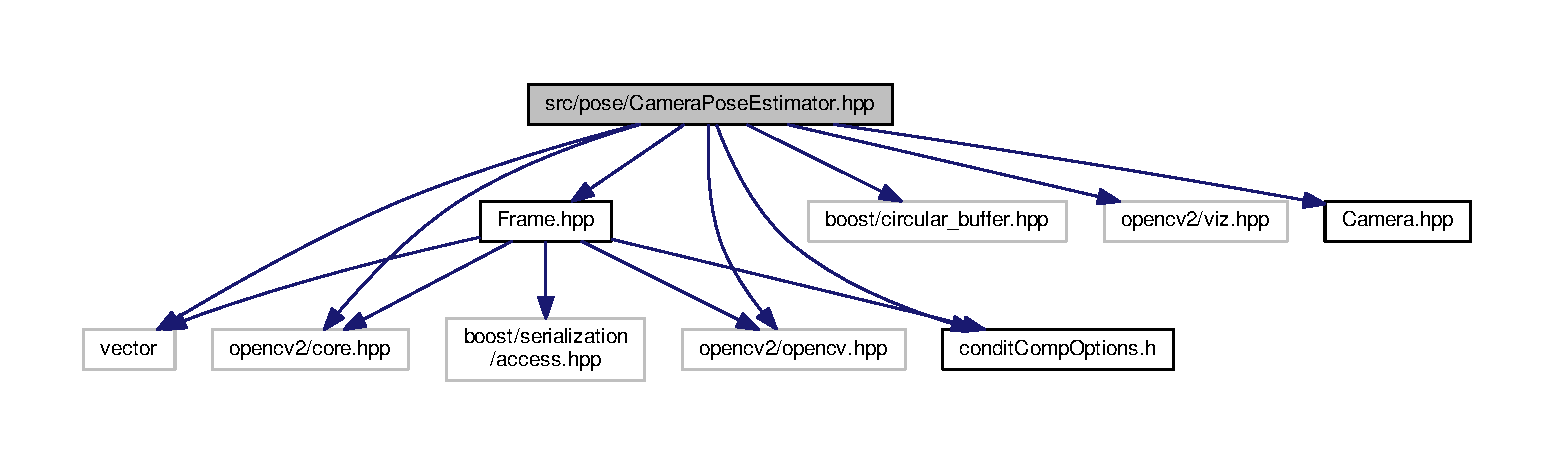
\includegraphics[width=350pt]{CameraPoseEstimator_8hpp__incl}
\end{center}
\end{figure}
This graph shows which files directly or indirectly include this file\+:\nopagebreak
\begin{figure}[H]
\begin{center}
\leavevmode
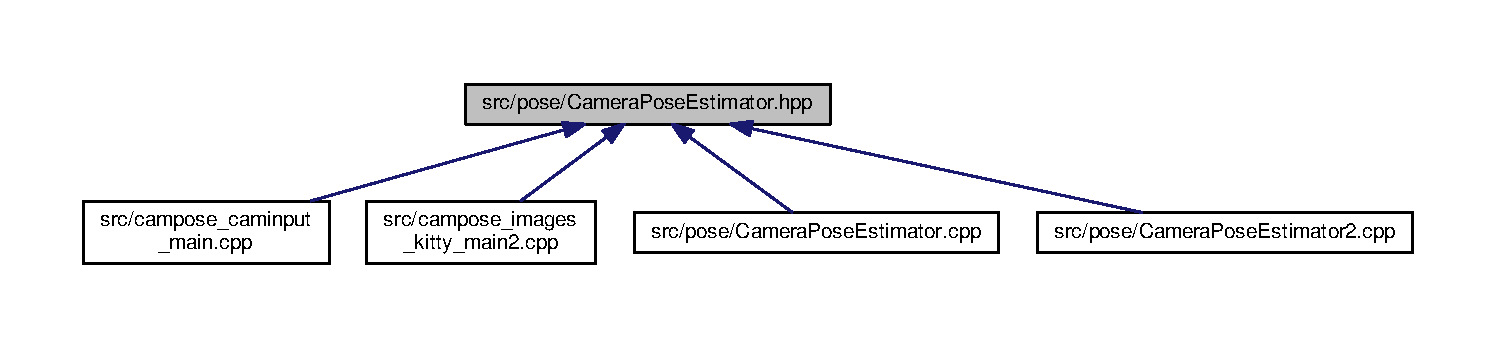
\includegraphics[width=350pt]{CameraPoseEstimator_8hpp__dep__incl}
\end{center}
\end{figure}
\subsection*{Classes}
\begin{DoxyCompactItemize}
\item 
class \hyperlink{classcampose_1_1CameraPoseEstimator}{campose\+::\+Camera\+Pose\+Estimator}
\end{DoxyCompactItemize}
\subsection*{Namespaces}
\begin{DoxyCompactItemize}
\item 
 \hyperlink{namespacecampose}{campose}
\end{DoxyCompactItemize}

\hypertarget{CameraPoseEstimator2_8cpp}{}\section{src/pose/\+Camera\+Pose\+Estimator2.cpp File Reference}
\label{CameraPoseEstimator2_8cpp}\index{src/pose/\+Camera\+Pose\+Estimator2.\+cpp@{src/pose/\+Camera\+Pose\+Estimator2.\+cpp}}
{\ttfamily \#include $<$string$>$}\\*
{\ttfamily \#include $<$iostream$>$}\\*
{\ttfamily \#include \char`\"{}Camera\+Pose\+Estimator.\+hpp\char`\"{}}\\*
{\ttfamily \#include \char`\"{}opencv2/calib3d.\+hpp\char`\"{}}\\*
{\ttfamily \#include $<$opencv2/viz.\+hpp$>$}\\*
{\ttfamily \#include $<$opencv2/viz/widgets.\+hpp$>$}\\*
{\ttfamily \#include $<$opencv2/core/types.\+hpp$>$}\\*
{\ttfamily \#include \char`\"{}triangulate.\+h\char`\"{}}\\*
Include dependency graph for Camera\+Pose\+Estimator2.\+cpp\+:\nopagebreak
\begin{figure}[H]
\begin{center}
\leavevmode
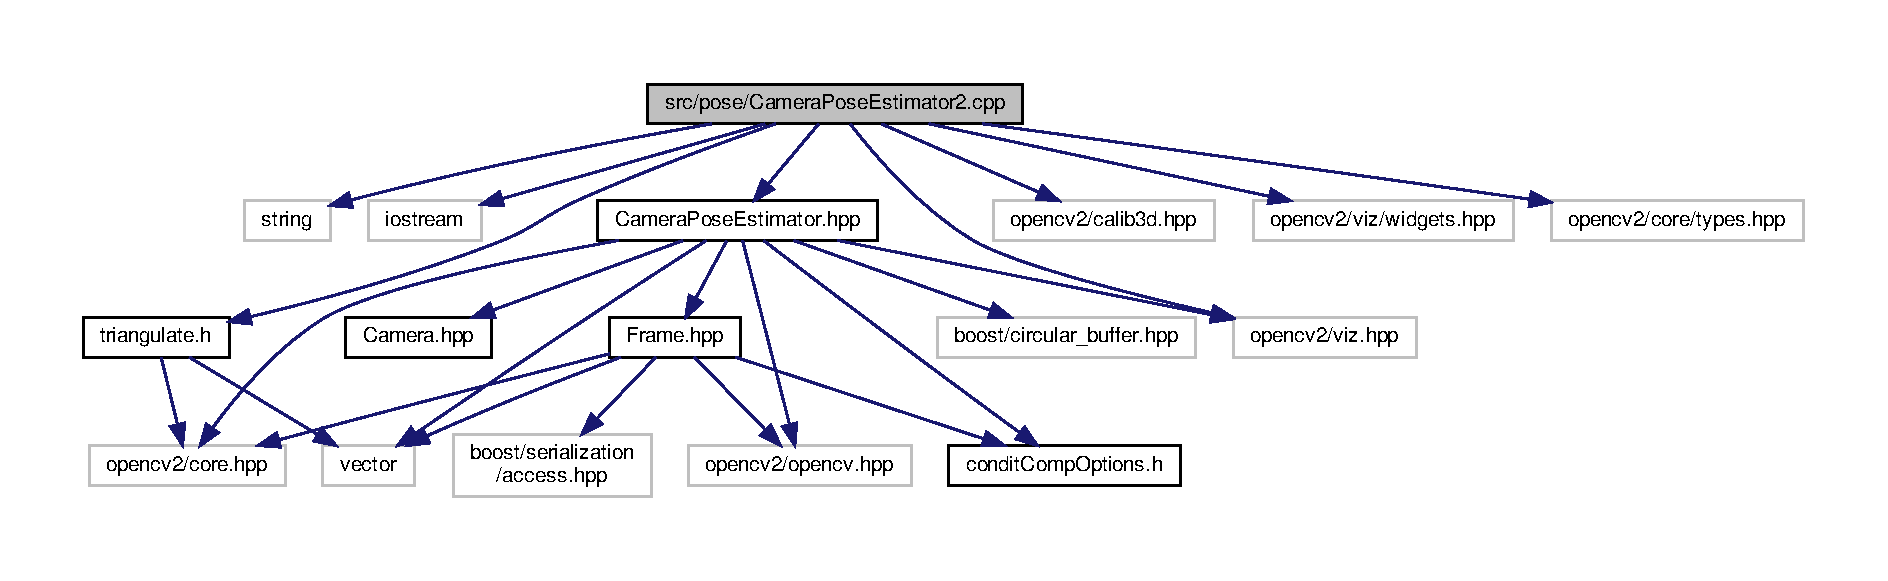
\includegraphics[width=350pt]{CameraPoseEstimator2_8cpp__incl}
\end{center}
\end{figure}

\hypertarget{CameraPoseEstimator2_8hpp}{}\section{src/pose/\+Camera\+Pose\+Estimator2.hpp File Reference}
\label{CameraPoseEstimator2_8hpp}\index{src/pose/\+Camera\+Pose\+Estimator2.\+hpp@{src/pose/\+Camera\+Pose\+Estimator2.\+hpp}}
{\ttfamily \#include $<$vector$>$}\\*
{\ttfamily \#include $<$opencv2/core.\+hpp$>$}\\*
{\ttfamily \#include \char`\"{}opencv2/opencv.\+hpp\char`\"{}}\\*
{\ttfamily \#include $<$boost/circular\+\_\+buffer.\+hpp$>$}\\*
{\ttfamily \#include $<$opencv2/viz.\+hpp$>$}\\*
{\ttfamily \#include \char`\"{}data\+Structures.\+h\char`\"{}}\\*
Include dependency graph for Camera\+Pose\+Estimator2.\+hpp\+:\nopagebreak
\begin{figure}[H]
\begin{center}
\leavevmode
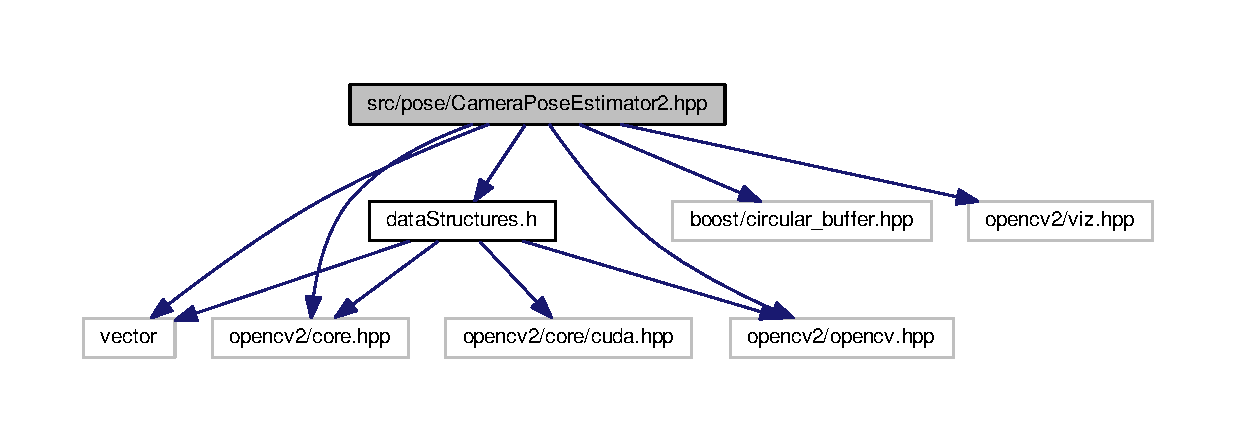
\includegraphics[width=350pt]{CameraPoseEstimator2_8hpp__incl}
\end{center}
\end{figure}
\subsection*{Classes}
\begin{DoxyCompactItemize}
\item 
class \hyperlink{classCameraPoseEstimator}{Camera\+Pose\+Estimator}
\end{DoxyCompactItemize}
\subsection*{Macros}
\begin{DoxyCompactItemize}
\item 
\#define \hyperlink{CameraPoseEstimator2_8hpp_a187e7ebc8dda5a3d55fbcaa1efea149a}{U\+N\+D\+I\+S\+T\+O\+R\+T\+E\+D\+\_\+\+P\+O\+I\+N\+T\+\_\+\+N\+BR}~(0)
\end{DoxyCompactItemize}


\subsection{Macro Definition Documentation}
\index{Camera\+Pose\+Estimator2.\+hpp@{Camera\+Pose\+Estimator2.\+hpp}!U\+N\+D\+I\+S\+T\+O\+R\+T\+E\+D\+\_\+\+P\+O\+I\+N\+T\+\_\+\+N\+BR@{U\+N\+D\+I\+S\+T\+O\+R\+T\+E\+D\+\_\+\+P\+O\+I\+N\+T\+\_\+\+N\+BR}}
\index{U\+N\+D\+I\+S\+T\+O\+R\+T\+E\+D\+\_\+\+P\+O\+I\+N\+T\+\_\+\+N\+BR@{U\+N\+D\+I\+S\+T\+O\+R\+T\+E\+D\+\_\+\+P\+O\+I\+N\+T\+\_\+\+N\+BR}!Camera\+Pose\+Estimator2.\+hpp@{Camera\+Pose\+Estimator2.\+hpp}}
\subsubsection[{\texorpdfstring{U\+N\+D\+I\+S\+T\+O\+R\+T\+E\+D\+\_\+\+P\+O\+I\+N\+T\+\_\+\+N\+BR}{UNDISTORTED_POINT_NBR}}]{\setlength{\rightskip}{0pt plus 5cm}\#define U\+N\+D\+I\+S\+T\+O\+R\+T\+E\+D\+\_\+\+P\+O\+I\+N\+T\+\_\+\+N\+BR~(0)}\hypertarget{CameraPoseEstimator2_8hpp_a187e7ebc8dda5a3d55fbcaa1efea149a}{}\label{CameraPoseEstimator2_8hpp_a187e7ebc8dda5a3d55fbcaa1efea149a}

\hypertarget{conditCompOptions_8h}{}\section{src/pose/condit\+Comp\+Options.h File Reference}
\label{conditCompOptions_8h}\index{src/pose/condit\+Comp\+Options.\+h@{src/pose/condit\+Comp\+Options.\+h}}
This graph shows which files directly or indirectly include this file\+:\nopagebreak
\begin{figure}[H]
\begin{center}
\leavevmode
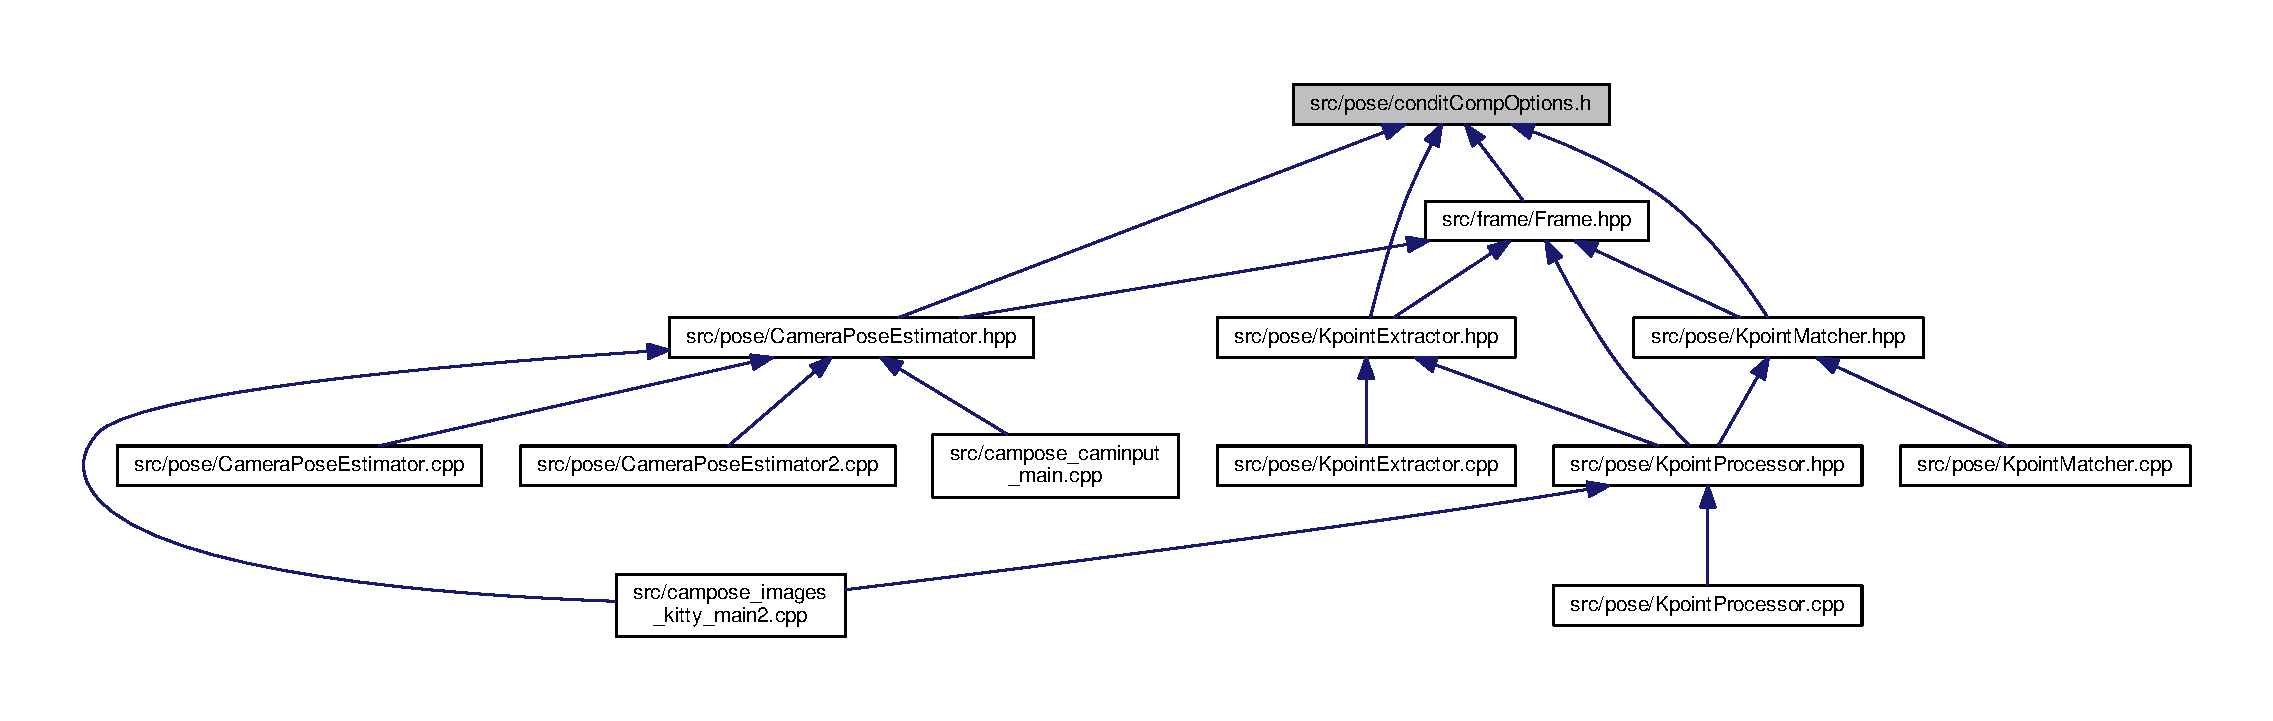
\includegraphics[width=350pt]{conditCompOptions_8h__dep__incl}
\end{center}
\end{figure}
\subsection*{Macros}
\begin{DoxyCompactItemize}
\item 
\#define \hyperlink{conditCompOptions_8h_aa33c965c87892b40c2bfdcbdc554c919}{D\+E\+B\+U\+G\+\_\+\+L\+A\+T\+E\+N\+CY}~(1)
\item 
\#define \hyperlink{conditCompOptions_8h_a2ed407574039ba810b9b58949ee97eeb}{E\+N\+A\+B\+L\+E\+\_\+\+V\+I\+SU}~(1)
\end{DoxyCompactItemize}


\subsection{Macro Definition Documentation}
\mbox{\Hypertarget{conditCompOptions_8h_aa33c965c87892b40c2bfdcbdc554c919}\label{conditCompOptions_8h_aa33c965c87892b40c2bfdcbdc554c919}} 
\index{condit\+Comp\+Options.\+h@{condit\+Comp\+Options.\+h}!D\+E\+B\+U\+G\+\_\+\+L\+A\+T\+E\+N\+CY@{D\+E\+B\+U\+G\+\_\+\+L\+A\+T\+E\+N\+CY}}
\index{D\+E\+B\+U\+G\+\_\+\+L\+A\+T\+E\+N\+CY@{D\+E\+B\+U\+G\+\_\+\+L\+A\+T\+E\+N\+CY}!condit\+Comp\+Options.\+h@{condit\+Comp\+Options.\+h}}
\subsubsection{\texorpdfstring{D\+E\+B\+U\+G\+\_\+\+L\+A\+T\+E\+N\+CY}{DEBUG\_LATENCY}}
{\footnotesize\ttfamily \#define D\+E\+B\+U\+G\+\_\+\+L\+A\+T\+E\+N\+CY~(1)}

\mbox{\Hypertarget{conditCompOptions_8h_a2ed407574039ba810b9b58949ee97eeb}\label{conditCompOptions_8h_a2ed407574039ba810b9b58949ee97eeb}} 
\index{condit\+Comp\+Options.\+h@{condit\+Comp\+Options.\+h}!E\+N\+A\+B\+L\+E\+\_\+\+V\+I\+SU@{E\+N\+A\+B\+L\+E\+\_\+\+V\+I\+SU}}
\index{E\+N\+A\+B\+L\+E\+\_\+\+V\+I\+SU@{E\+N\+A\+B\+L\+E\+\_\+\+V\+I\+SU}!condit\+Comp\+Options.\+h@{condit\+Comp\+Options.\+h}}
\subsubsection{\texorpdfstring{E\+N\+A\+B\+L\+E\+\_\+\+V\+I\+SU}{ENABLE\_VISU}}
{\footnotesize\ttfamily \#define E\+N\+A\+B\+L\+E\+\_\+\+V\+I\+SU~(1)}


\hypertarget{KeypointProcessorGpu_8cpp}{}\section{src/pose/\+Keypoint\+Processor\+Gpu.cpp File Reference}
\label{KeypointProcessorGpu_8cpp}\index{src/pose/\+Keypoint\+Processor\+Gpu.\+cpp@{src/pose/\+Keypoint\+Processor\+Gpu.\+cpp}}
{\ttfamily \#include \char`\"{}Keypoint\+Processor\+Gpu.\+hpp\char`\"{}}\newline
{\ttfamily \#include $<$vector$>$}\newline
{\ttfamily \#include $<$opencv2/core.\+hpp$>$}\newline
{\ttfamily \#include \char`\"{}opencv2/opencv.\+hpp\char`\"{}}\newline
{\ttfamily \#include $<$opencv2/features2d.\+hpp$>$}\newline
{\ttfamily \#include $<$opencv2/xfeatures2d.\+hpp$>$}\newline
{\ttfamily \#include $<$opencv2/xfeatures2d/nonfree.\+hpp$>$}\newline
{\ttfamily \#include $<$opencv2/calib3d.\+hpp$>$}\newline
Include dependency graph for Keypoint\+Processor\+Gpu.\+cpp\+:\nopagebreak
\begin{figure}[H]
\begin{center}
\leavevmode
\includegraphics[width=350pt]{KeypointProcessorGpu_8cpp__incl}
\end{center}
\end{figure}

\hypertarget{KeypointProcessorGpu_8hpp}{}\section{src/pose/\+Keypoint\+Processor\+Gpu.hpp File Reference}
\label{KeypointProcessorGpu_8hpp}\index{src/pose/\+Keypoint\+Processor\+Gpu.\+hpp@{src/pose/\+Keypoint\+Processor\+Gpu.\+hpp}}
{\ttfamily \#include $<$string$>$}\\*
{\ttfamily \#include $<$boost/circular\+\_\+buffer.\+hpp$>$}\\*
{\ttfamily \#include $<$opencv2/core/cuda.\+hpp$>$}\\*
{\ttfamily \#include \char`\"{}data\+Structures.\+h\char`\"{}}\\*
Include dependency graph for Keypoint\+Processor\+Gpu.\+hpp\+:\nopagebreak
\begin{figure}[H]
\begin{center}
\leavevmode
\includegraphics[width=350pt]{KeypointProcessorGpu_8hpp__incl}
\end{center}
\end{figure}
This graph shows which files directly or indirectly include this file\+:\nopagebreak
\begin{figure}[H]
\begin{center}
\leavevmode
\includegraphics[width=350pt]{KeypointProcessorGpu_8hpp__dep__incl}
\end{center}
\end{figure}
\subsection*{Classes}
\begin{DoxyCompactItemize}
\item 
class \hyperlink{classKeypointProcessorGpu}{Keypoint\+Processor\+Gpu}
\end{DoxyCompactItemize}
\subsection*{Namespaces}
\begin{DoxyCompactItemize}
\item 
 \hyperlink{namespaceRefineReturnCode}{Refine\+Return\+Code}
\item 
 \hyperlink{namespaceExtractReturnCode}{Extract\+Return\+Code}
\item 
 \hyperlink{namespaceFrameSTS}{Frame\+S\+TS}
\end{DoxyCompactItemize}
\subsection*{Enumerations}
\begin{DoxyCompactItemize}
\item 
enum \hyperlink{namespaceRefineReturnCode_a54e2cd5f4af90ff2df55bf63455d1959}{Refine\+Return\+Code\+::\+Refine\+Return\+Code} \{ \hyperlink{namespaceRefineReturnCode_a54e2cd5f4af90ff2df55bf63455d1959af7afdc3f9a9d0e3ee3e177cf5f5f9841}{Refine\+Return\+Code\+::\+OK} = 0, 
\hyperlink{namespaceRefineReturnCode_a54e2cd5f4af90ff2df55bf63455d1959aa7e9b732c19c32b516e07f10aedd581c}{Refine\+Return\+Code\+::\+N\+O\+T\+\_\+\+E\+N\+O\+U\+G\+H\+\_\+\+I\+N\+L\+I\+E\+RS} = -\/1
 \}
\item 
enum \hyperlink{namespaceExtractReturnCode_a88d3d56de717f250bf48793769dd57ba}{Extract\+Return\+Code\+::\+Extract\+Return\+Code} \{ \hyperlink{namespaceExtractReturnCode_a88d3d56de717f250bf48793769dd57baa35e3ef3fef8fcb5cc35f89bcdbf50d5a}{Extract\+Return\+Code\+::\+OK} = 0, 
\hyperlink{namespaceExtractReturnCode_a88d3d56de717f250bf48793769dd57baacc16e5e7772072e33bf927abd7c422c6}{Extract\+Return\+Code\+::\+N\+O\+T\+\_\+\+E\+N\+O\+U\+G\+H\+\_\+\+K\+E\+Y\+P\+O\+I\+N\+TS} = -\/1
 \}
\item 
enum \hyperlink{namespaceFrameSTS_aa00e1583f3bc837ad3fbfb9beaaa0692}{Frame\+S\+T\+S\+::\+Frame\+S\+TS} \{ \hyperlink{namespaceFrameSTS_aa00e1583f3bc837ad3fbfb9beaaa0692a8608718df5a4cb285e39336cb325e5b9}{Frame\+S\+T\+S\+::\+D\+I\+S\+C\+A\+R\+D\+ED} = -\/1, 
\hyperlink{namespaceFrameSTS_aa00e1583f3bc837ad3fbfb9beaaa0692a8320d47ecf7adbfb6dedd682bf1820db}{Frame\+S\+T\+S\+::\+N\+O\+T\+\_\+\+Y\+E\+T\+\_\+\+P\+R\+O\+C\+E\+S\+S\+ED} = 0, 
\hyperlink{namespaceFrameSTS_aa00e1583f3bc837ad3fbfb9beaaa0692a68c0ae2c9cca0d93791d8493061f4d95}{Frame\+S\+T\+S\+::\+P\+R\+O\+C\+E\+S\+S\+ED} = 1
 \}
\end{DoxyCompactItemize}

\hypertarget{KpointExtractor_8cpp}{}\section{src/pose/\+Kpoint\+Extractor.cpp File Reference}
\label{KpointExtractor_8cpp}\index{src/pose/\+Kpoint\+Extractor.\+cpp@{src/pose/\+Kpoint\+Extractor.\+cpp}}


keypoints extractor implementation file.  


{\ttfamily \#include \char`\"{}Kpoint\+Extractor.\+hpp\char`\"{}}\\*
Include dependency graph for Kpoint\+Extractor.\+cpp\+:\nopagebreak
\begin{figure}[H]
\begin{center}
\leavevmode
\includegraphics[width=350pt]{KpointExtractor_8cpp__incl}
\end{center}
\end{figure}


\subsection{Detailed Description}
keypoints extractor implementation file. 


\hypertarget{KpointExtractor_8hpp}{}\section{src/pose/\+Kpoint\+Extractor.hpp File Reference}
\label{KpointExtractor_8hpp}\index{src/pose/\+Kpoint\+Extractor.\+hpp@{src/pose/\+Kpoint\+Extractor.\+hpp}}


Header file for lass to extract keypoints.  


{\ttfamily \#include \char`\"{}data\+Structures.\+h\char`\"{}}\newline
{\ttfamily \#include \char`\"{}Frame.\+hpp\char`\"{}}\newline
{\ttfamily \#include \char`\"{}condit\+Comp\+Options.\+h\char`\"{}}\newline
Include dependency graph for Kpoint\+Extractor.\+hpp\+:\nopagebreak
\begin{figure}[H]
\begin{center}
\leavevmode
\includegraphics[width=350pt]{KpointExtractor_8hpp__incl}
\end{center}
\end{figure}
This graph shows which files directly or indirectly include this file\+:\nopagebreak
\begin{figure}[H]
\begin{center}
\leavevmode
\includegraphics[width=350pt]{KpointExtractor_8hpp__dep__incl}
\end{center}
\end{figure}
\subsection*{Classes}
\begin{DoxyCompactItemize}
\item 
class \hyperlink{classkpproc_1_1KpointExtractor}{kpproc\+::\+Kpoint\+Extractor}
\end{DoxyCompactItemize}
\subsection*{Namespaces}
\begin{DoxyCompactItemize}
\item 
 \hyperlink{namespacekpproc}{kpproc}
\end{DoxyCompactItemize}


\subsection{Detailed Description}
Header file for lass to extract keypoints. 


\hypertarget{KpointMatcher_8cpp}{}\section{src/pose/\+Kpoint\+Matcher.cpp File Reference}
\label{KpointMatcher_8cpp}\index{src/pose/\+Kpoint\+Matcher.\+cpp@{src/pose/\+Kpoint\+Matcher.\+cpp}}
{\ttfamily \#include \char`\"{}Kpoint\+Matcher.\+hpp\char`\"{}}\newline
Include dependency graph for Kpoint\+Matcher.\+cpp\+:\nopagebreak
\begin{figure}[H]
\begin{center}
\leavevmode
\includegraphics[width=350pt]{KpointMatcher_8cpp__incl}
\end{center}
\end{figure}

\hypertarget{KpointMatcher_8hpp}{}\section{src/pose/\+Kpoint\+Matcher.hpp File Reference}
\label{KpointMatcher_8hpp}\index{src/pose/\+Kpoint\+Matcher.\+hpp@{src/pose/\+Kpoint\+Matcher.\+hpp}}


Header file for lass to match keypoints.  


{\ttfamily \#include \char`\"{}Frame.\+hpp\char`\"{}}\\*
{\ttfamily \#include \char`\"{}condit\+Comp\+Options.\+h\char`\"{}}\\*
Include dependency graph for Kpoint\+Matcher.\+hpp\+:
\nopagebreak
\begin{figure}[H]
\begin{center}
\leavevmode
\includegraphics[width=350pt]{KpointMatcher_8hpp__incl}
\end{center}
\end{figure}
This graph shows which files directly or indirectly include this file\+:\nopagebreak
\begin{figure}[H]
\begin{center}
\leavevmode
\includegraphics[width=350pt]{KpointMatcher_8hpp__dep__incl}
\end{center}
\end{figure}
\subsection*{Classes}
\begin{DoxyCompactItemize}
\item 
class \hyperlink{classkpproc_1_1KpointMatcher}{kpproc\+::\+Kpoint\+Matcher}
\end{DoxyCompactItemize}
\subsection*{Namespaces}
\begin{DoxyCompactItemize}
\item 
 \hyperlink{namespacekpproc}{kpproc}
\end{DoxyCompactItemize}


\subsection{Detailed Description}
Header file for lass to match keypoints. 


\hypertarget{KpointProcessor_8cpp}{}\section{src/pose/\+Kpoint\+Processor.cpp File Reference}
\label{KpointProcessor_8cpp}\index{src/pose/\+Kpoint\+Processor.\+cpp@{src/pose/\+Kpoint\+Processor.\+cpp}}
{\ttfamily \#include \char`\"{}Kpoint\+Processor.\+hpp\char`\"{}}\newline
Include dependency graph for Kpoint\+Processor.\+cpp\+:\nopagebreak
\begin{figure}[H]
\begin{center}
\leavevmode
\includegraphics[width=350pt]{KpointProcessor_8cpp__incl}
\end{center}
\end{figure}

\hypertarget{KpointProcessor_8hpp}{}\section{src/pose/\+Kpoint\+Processor.hpp File Reference}
\label{KpointProcessor_8hpp}\index{src/pose/\+Kpoint\+Processor.\+hpp@{src/pose/\+Kpoint\+Processor.\+hpp}}
{\ttfamily \#include $<$boost/circular\+\_\+buffer.\+hpp$>$}\\*
{\ttfamily \#include \char`\"{}Kpoint\+Extractor.\+hpp\char`\"{}}\\*
{\ttfamily \#include \char`\"{}Kpoint\+Matcher.\+hpp\char`\"{}}\\*
{\ttfamily \#include \char`\"{}Frame.\+hpp\char`\"{}}\\*
Include dependency graph for Kpoint\+Processor.\+hpp\+:
\nopagebreak
\begin{figure}[H]
\begin{center}
\leavevmode
\includegraphics[width=350pt]{KpointProcessor_8hpp__incl}
\end{center}
\end{figure}
This graph shows which files directly or indirectly include this file\+:\nopagebreak
\begin{figure}[H]
\begin{center}
\leavevmode
\includegraphics[width=350pt]{KpointProcessor_8hpp__dep__incl}
\end{center}
\end{figure}
\subsection*{Classes}
\begin{DoxyCompactItemize}
\item 
class \hyperlink{classkpproc_1_1KpointProcessor}{kpproc\+::\+Kpoint\+Processor}
\end{DoxyCompactItemize}
\subsection*{Namespaces}
\begin{DoxyCompactItemize}
\item 
 \hyperlink{namespacekpproc}{kpproc}
\end{DoxyCompactItemize}

\hypertarget{triangulate_8cpp}{}\section{src/pose/triangulate.cpp File Reference}
\label{triangulate_8cpp}\index{src/pose/triangulate.\+cpp@{src/pose/triangulate.\+cpp}}
{\ttfamily \#include \char`\"{}triangulate.\+h\char`\"{}}\newline
Include dependency graph for triangulate.\+cpp\+:\nopagebreak
\begin{figure}[H]
\begin{center}
\leavevmode
\includegraphics[width=236pt]{triangulate_8cpp__incl}
\end{center}
\end{figure}
\subsection*{Functions}
\begin{DoxyCompactItemize}
\item 
cv\+::\+Vec3d \hyperlink{triangulate_8cpp_a019ddf1a098d0ee9b1054d0e63ff9602}{triangulate} (const cv\+::\+Mat \&p1, const cv\+::\+Mat \&p2, const cv\+::\+Vec2d \&u1, const cv\+::\+Vec2d \&u2)
\item 
void \hyperlink{triangulate_8cpp_ac6bf3148088f8b4af058341b633ae0a3}{triangulate} (const cv\+::\+Mat \&p1, const cv\+::\+Mat \&p2, const std\+::vector$<$ cv\+::\+Vec2d $>$ \&pts1, const std\+::vector$<$ cv\+::\+Vec2d $>$ \&pts2, std\+::vector$<$ cv\+::\+Vec3d $>$ \&pts3D)
\end{DoxyCompactItemize}


\subsection{Function Documentation}
\mbox{\Hypertarget{triangulate_8cpp_a019ddf1a098d0ee9b1054d0e63ff9602}\label{triangulate_8cpp_a019ddf1a098d0ee9b1054d0e63ff9602}} 
\index{triangulate.\+cpp@{triangulate.\+cpp}!triangulate@{triangulate}}
\index{triangulate@{triangulate}!triangulate.\+cpp@{triangulate.\+cpp}}
\subsubsection{\texorpdfstring{triangulate()}{triangulate()}\hspace{0.1cm}{\footnotesize\ttfamily [1/2]}}
{\footnotesize\ttfamily cv\+::\+Vec3d triangulate (\begin{DoxyParamCaption}\item[{const cv\+::\+Mat \&}]{p1,  }\item[{const cv\+::\+Mat \&}]{p2,  }\item[{const cv\+::\+Vec2d \&}]{u1,  }\item[{const cv\+::\+Vec2d \&}]{u2 }\end{DoxyParamCaption})}

Here is the caller graph for this function\+:\nopagebreak
\begin{figure}[H]
\begin{center}
\leavevmode
\includegraphics[width=350pt]{triangulate_8cpp_a019ddf1a098d0ee9b1054d0e63ff9602_icgraph}
\end{center}
\end{figure}
\mbox{\Hypertarget{triangulate_8cpp_ac6bf3148088f8b4af058341b633ae0a3}\label{triangulate_8cpp_ac6bf3148088f8b4af058341b633ae0a3}} 
\index{triangulate.\+cpp@{triangulate.\+cpp}!triangulate@{triangulate}}
\index{triangulate@{triangulate}!triangulate.\+cpp@{triangulate.\+cpp}}
\subsubsection{\texorpdfstring{triangulate()}{triangulate()}\hspace{0.1cm}{\footnotesize\ttfamily [2/2]}}
{\footnotesize\ttfamily void triangulate (\begin{DoxyParamCaption}\item[{const cv\+::\+Mat \&}]{p1,  }\item[{const cv\+::\+Mat \&}]{p2,  }\item[{const std\+::vector$<$ cv\+::\+Vec2d $>$ \&}]{pts1,  }\item[{const std\+::vector$<$ cv\+::\+Vec2d $>$ \&}]{pts2,  }\item[{std\+::vector$<$ cv\+::\+Vec3d $>$ \&}]{pts3D }\end{DoxyParamCaption})}

Here is the call graph for this function\+:\nopagebreak
\begin{figure}[H]
\begin{center}
\leavevmode
\includegraphics[width=240pt]{triangulate_8cpp_ac6bf3148088f8b4af058341b633ae0a3_cgraph}
\end{center}
\end{figure}

\hypertarget{triangulate_8h}{}\section{src/pose/triangulate.h File Reference}
\label{triangulate_8h}\index{src/pose/triangulate.\+h@{src/pose/triangulate.\+h}}
{\ttfamily \#include $<$opencv2/core.\+hpp$>$}\newline
{\ttfamily \#include $<$vector$>$}\newline
Include dependency graph for triangulate.\+h\+:\nopagebreak
\begin{figure}[H]
\begin{center}
\leavevmode
\includegraphics[width=236pt]{triangulate_8h__incl}
\end{center}
\end{figure}
This graph shows which files directly or indirectly include this file\+:\nopagebreak
\begin{figure}[H]
\begin{center}
\leavevmode
\includegraphics[width=350pt]{triangulate_8h__dep__incl}
\end{center}
\end{figure}
\subsection*{Functions}
\begin{DoxyCompactItemize}
\item 
cv\+::\+Vec3d \hyperlink{triangulate_8h_a019ddf1a098d0ee9b1054d0e63ff9602}{triangulate} (const cv\+::\+Mat \&p1, const cv\+::\+Mat \&p2, const cv\+::\+Vec2d \&u1, const cv\+::\+Vec2d \&u2)
\item 
void \hyperlink{triangulate_8h_ac6bf3148088f8b4af058341b633ae0a3}{triangulate} (const cv\+::\+Mat \&p1, const cv\+::\+Mat \&p2, const std\+::vector$<$ cv\+::\+Vec2d $>$ \&pts1, const std\+::vector$<$ cv\+::\+Vec2d $>$ \&pts2, std\+::vector$<$ cv\+::\+Vec3d $>$ \&pts3D)
\end{DoxyCompactItemize}


\subsection{Function Documentation}
\mbox{\Hypertarget{triangulate_8h_a019ddf1a098d0ee9b1054d0e63ff9602}\label{triangulate_8h_a019ddf1a098d0ee9b1054d0e63ff9602}} 
\index{triangulate.\+h@{triangulate.\+h}!triangulate@{triangulate}}
\index{triangulate@{triangulate}!triangulate.\+h@{triangulate.\+h}}
\subsubsection{\texorpdfstring{triangulate()}{triangulate()}\hspace{0.1cm}{\footnotesize\ttfamily [1/2]}}
{\footnotesize\ttfamily cv\+::\+Vec3d triangulate (\begin{DoxyParamCaption}\item[{const cv\+::\+Mat \&}]{p1,  }\item[{const cv\+::\+Mat \&}]{p2,  }\item[{const cv\+::\+Vec2d \&}]{u1,  }\item[{const cv\+::\+Vec2d \&}]{u2 }\end{DoxyParamCaption})}

Here is the caller graph for this function\+:\nopagebreak
\begin{figure}[H]
\begin{center}
\leavevmode
\includegraphics[width=350pt]{triangulate_8h_a019ddf1a098d0ee9b1054d0e63ff9602_icgraph}
\end{center}
\end{figure}
\mbox{\Hypertarget{triangulate_8h_ac6bf3148088f8b4af058341b633ae0a3}\label{triangulate_8h_ac6bf3148088f8b4af058341b633ae0a3}} 
\index{triangulate.\+h@{triangulate.\+h}!triangulate@{triangulate}}
\index{triangulate@{triangulate}!triangulate.\+h@{triangulate.\+h}}
\subsubsection{\texorpdfstring{triangulate()}{triangulate()}\hspace{0.1cm}{\footnotesize\ttfamily [2/2]}}
{\footnotesize\ttfamily void triangulate (\begin{DoxyParamCaption}\item[{const cv\+::\+Mat \&}]{p1,  }\item[{const cv\+::\+Mat \&}]{p2,  }\item[{const std\+::vector$<$ cv\+::\+Vec2d $>$ \&}]{pts1,  }\item[{const std\+::vector$<$ cv\+::\+Vec2d $>$ \&}]{pts2,  }\item[{std\+::vector$<$ cv\+::\+Vec3d $>$ \&}]{pts3D }\end{DoxyParamCaption})}

Here is the call graph for this function\+:\nopagebreak
\begin{figure}[H]
\begin{center}
\leavevmode
\includegraphics[width=240pt]{triangulate_8h_ac6bf3148088f8b4af058341b633ae0a3_cgraph}
\end{center}
\end{figure}

%--- End generated contents ---

% Index
\backmatter
\newpage
\phantomsection
\clearemptydoublepage
\addcontentsline{toc}{chapter}{Index}
\printindex

\end{document}
